\documentclass[twoside]{book}

% Packages required by doxygen
\usepackage{fixltx2e}
\usepackage{calc}
\usepackage{doxygen}
\usepackage[export]{adjustbox} % also loads graphicx
\usepackage{graphicx}
\usepackage[utf8]{inputenc}
\usepackage{makeidx}
\usepackage{multicol}
\usepackage{multirow}
\PassOptionsToPackage{warn}{textcomp}
\usepackage{textcomp}
\usepackage[nointegrals]{wasysym}
\usepackage[table]{xcolor}

% Font selection
\usepackage[T1]{fontenc}
\usepackage[scaled=.90]{helvet}
\usepackage{courier}
\usepackage{amssymb}
\usepackage{sectsty}
\renewcommand{\familydefault}{\sfdefault}
\allsectionsfont{%
  \fontseries{bc}\selectfont%
  \color{darkgray}%
}
\renewcommand{\DoxyLabelFont}{%
  \fontseries{bc}\selectfont%
  \color{darkgray}%
}
\newcommand{\+}{\discretionary{\mbox{\scriptsize$\hookleftarrow$}}{}{}}

% Page & text layout
\usepackage{geometry}
\geometry{%
  a4paper,%
  top=2.5cm,%
  bottom=2.5cm,%
  left=2.5cm,%
  right=2.5cm%
}
\tolerance=750
\hfuzz=15pt
\hbadness=750
\setlength{\emergencystretch}{15pt}
\setlength{\parindent}{0cm}
\setlength{\parskip}{0.2cm}
\makeatletter
\renewcommand{\paragraph}{%
  \@startsection{paragraph}{4}{0ex}{-1.0ex}{1.0ex}{%
    \normalfont\normalsize\bfseries\SS@parafont%
  }%
}
\renewcommand{\subparagraph}{%
  \@startsection{subparagraph}{5}{0ex}{-1.0ex}{1.0ex}{%
    \normalfont\normalsize\bfseries\SS@subparafont%
  }%
}
\makeatother

% Headers & footers
\usepackage{fancyhdr}
\pagestyle{fancyplain}
\fancyhead[LE]{\fancyplain{}{\bfseries\thepage}}
\fancyhead[CE]{\fancyplain{}{}}
\fancyhead[RE]{\fancyplain{}{\bfseries\leftmark}}
\fancyhead[LO]{\fancyplain{}{\bfseries\rightmark}}
\fancyhead[CO]{\fancyplain{}{}}
\fancyhead[RO]{\fancyplain{}{\bfseries\thepage}}
\fancyfoot[LE]{\fancyplain{}{}}
\fancyfoot[CE]{\fancyplain{}{}}
\fancyfoot[RE]{\fancyplain{}{\bfseries\scriptsize Generated on Tue Sep 29 2015 10\+:26\+:57 for Crystal Builder v 3.\+7.\+0 by Doxygen }}
\fancyfoot[LO]{\fancyplain{}{\bfseries\scriptsize Generated on Tue Sep 29 2015 10\+:26\+:57 for Crystal Builder v 3.\+7.\+0 by Doxygen }}
\fancyfoot[CO]{\fancyplain{}{}}
\fancyfoot[RO]{\fancyplain{}{}}
\renewcommand{\footrulewidth}{0.4pt}
\renewcommand{\chaptermark}[1]{%
  \markboth{#1}{}%
}
\renewcommand{\sectionmark}[1]{%
  \markright{\thesection\ #1}%
}

% Indices & bibliography
\usepackage{natbib}
\usepackage[titles]{tocloft}
\setcounter{tocdepth}{3}
\setcounter{secnumdepth}{5}
\makeindex

% Hyperlinks (required, but should be loaded last)
\usepackage{ifpdf}
\ifpdf
  \usepackage[pdftex,pagebackref=true]{hyperref}
\else
  \usepackage[ps2pdf,pagebackref=true]{hyperref}
\fi
\hypersetup{%
  colorlinks=true,%
  linkcolor=blue,%
  citecolor=blue,%
  unicode%
}

% Custom commands
\newcommand{\clearemptydoublepage}{%
  \newpage{\pagestyle{empty}\cleardoublepage}%
}


%===== C O N T E N T S =====

\begin{document}

% Titlepage & ToC
\hypersetup{pageanchor=false,
             bookmarks=true,
             bookmarksnumbered=true,
             pdfencoding=unicode
            }
\pagenumbering{roman}
\begin{titlepage}
\vspace*{7cm}
\begin{center}%
{\Large Crystal Builder v 3.7.0 }\\
\vspace*{1cm}
{\large Generated by Doxygen 1.8.9.1}\\
\vspace*{0.5cm}
{\small Tue Sep 29 2015 10:26:57}\\
\end{center}
\end{titlepage}
\clearemptydoublepage
\tableofcontents
\clearemptydoublepage
\pagenumbering{arabic}
\hypersetup{pageanchor=true}

%--- Begin generated contents ---
\chapter{Main Page}
\label{index}\hypertarget{index}{}\subsection*{Capabilities}

\begin{DoxyVerb}Crystal Builder - Simple program to build several crystal structures for use in many popular 
molecular dynamics and denisty functional theory packages.  
\end{DoxyVerb}



\begin{DoxyItemize}
\item Bravais lattices\+: \hyperlink{class_cubic}{Cubic}, \hyperlink{class_orthorhombic}{Orthorhombic}, \hyperlink{class_tetragonal}{Tetragonal}
\item Library structures\+: ~\newline
 -\/ 2\+D materials\+: Graphene, h-\/\+B\+N, (M)etal (D)i(\+C)halcogenide-\/2\+H/1\+T (i.\+e. Sn\+S2), (T)ransition (M)etal (D)i(\+C)halcogenide-\/2\+H/1\+T (i.\+e. Mo\+Se2)~\newline
 -\/ Energetic materials (P\+E\+T\+N-\/\+I, T\+A\+T\+B, β-\/\+H\+M\+X)
\item Define a custom lattice by specifying the lattice parameters and angles, the basis positions, and the element types
\item Build and view large super cells (no limit on maximum atoms)
\item 3\+D graphics rendering of the crystals with real time user interaction
\item Display as a molecule or with a periodic unit cell
\item Display bonds between nearest neighbors, uniform cutoff
\item Print output atomic coordinates as fractional or cartesian
\item Output to several popular Denisty Functional Theory and Molecular Dynamics packages\+: ~\newline
 -\/ Materials Studio D\+Mol (.car) ~\newline
 -\/ L\+A\+M\+M\+P\+S (.input) ~\newline
 -\/ V\+A\+S\+P 5.\+x.\+x (P\+O\+S\+C\+A\+R)
\end{DoxyItemize}

N\+O\+T\+E\+: If you do not have the G\+T\+K+-\/2.0 libraries installed and in the usual path, i.\+e. {\ttfamily /usr/lib \& /usr/include} for Linux or as a {\ttfamily Framework} on Mac O\+S X, follow the directions below to install them.





\subsection*{Usage}

To use the program, simply execute the following in a terminal, \begin{DoxyVerb}    ./crysb  
\end{DoxyVerb}


Once the crystal has been defined and other relevant parameters are set, you can chose to simply build the crystal and have it saved to your file.

Alternatively, if the {\ttfamily Open G\+L} library was used in building this application, the crystal can be viewed in an interactive window by clicking the {\ttfamily Build+render} tab, see below for keyboard and mouse commands. Upon closing this rendering window the crystal data will be written to the file you specified and the main program will terminate.

\begin{DoxyVerb}    ** NOTE: If building a crystal with > 5000 atoms, rendering is a little slow.  Advise
             to use the build without rendering option.
\end{DoxyVerb}


\subsubsection*{Crystal/scene interaction}

\begin{DoxyVerb}    Mouse events:
      Left mouse            rotate/scale the object
      Right mouse           scene display menu
  
    Keyboard events:
        'A'                   display atoms and unit cell
        'a'                   display atoms only
        'B'                   display bonds, uniform nearest neighbor cutoff
        'b'                   hide bonds
        'C'                   increase nearest neighbor cutoff
        'c'                   decrease nearest neighbor cutoff
        'e'                   exit and save the data from the rendering scene
        'o'                   orthographic projection of the crystal
        'p'                   perspective projection of the crystal
        'r' then LeftButton   rotate the crystal in all 3 dimensions
        'W'                   change background to white and bounding box to black
        'w'                   change background to black and bounding box to white
        'z' then LeftButton   zoom toward/away from the crystal
        '0'                   reset orientation of crystal to looking down z toward xy plane
        '1'                   view the xz "a-c" plane of the crystal
        '2'                   view the yz "b-c" plane of the crystal
        '3'                   rotate crystal about x by -45˚, and then -45˚ about z, 'psuedo' perspective view
        '+'                   increase the particle radius uniformly
        '-'                   decrease the particle radius uniformly
   
        Up arrow              Shift the crystal in positive vertical screen direction
        Down arrow            Shift the crystal in negative vertical screen direction
        Left arrow            Shift the crystal in negative horizontal screen direction
        Right arrow           Shift the crystal in positive horizontal screen direction
\end{DoxyVerb}
 



\subsection*{Info }

{\bfseries Author\+:} \begin{DoxyVerb}/**
  * Joseph M. Gonzalez
  * PhD Student, Materials Simulation Laboratory
  * Department of Physics, University of South Florida, Tampa, FL 33620
  *
  * web: msl.cas.usf.edu
  */
\end{DoxyVerb}


{\bfseries Date\+:} Sep 27, 2015

{\bfseries email\+:} \href{mailto:jmgonza6@mail.usf.edu}{\tt jmgonza6@mail.\+usf.\+edu} 
\chapter{Namespace Index}
\section{Namespace List}
Here is a list of all namespaces with brief descriptions\+:\begin{DoxyCompactList}
\item\contentsline{section}{\hyperlink{namespace_m_a_t_h_n_s}{M\+A\+T\+H\+N\+S} \\*Customized math operations and interfaces }{\pageref{namespace_m_a_t_h_n_s}}{}
\end{DoxyCompactList}

\chapter{Hierarchical Index}
\section{Class Hierarchy}
This inheritance list is sorted roughly, but not completely, alphabetically\+:\begin{DoxyCompactList}
\item \contentsline{section}{atom\+\_\+t}{\pageref{structatom__t}}{}
\item \contentsline{section}{basis\+\_\+t}{\pageref{structbasis__t}}{}
\item \contentsline{section}{Errors}{\pageref{class_errors}}{}
\item \contentsline{section}{Gui}{\pageref{class_gui}}{}
\item \contentsline{section}{I\+N\+T\+E\+R\+F\+A\+C\+E}{\pageref{class_i_n_t_e_r_f_a_c_e}}{}
\item \contentsline{section}{L\+A\+T\+T\+I\+C\+E}{\pageref{class_l_a_t_t_i_c_e}}{}
\begin{DoxyCompactList}
\item \contentsline{section}{Cubic}{\pageref{class_cubic}}{}
\item \contentsline{section}{Custom}{\pageref{class_custom}}{}
\item \contentsline{section}{Hexagonal}{\pageref{class_hexagonal}}{}
\item \contentsline{section}{Orthorhombic}{\pageref{class_orthorhombic}}{}
\item \contentsline{section}{Structure\+Lib}{\pageref{class_structure_lib}}{}
\item \contentsline{section}{Tetragonal}{\pageref{class_tetragonal}}{}
\end{DoxyCompactList}
\item \contentsline{section}{Line}{\pageref{struct_line}}{}
\item \contentsline{section}{M\+E\+M\+O\+R\+Y}{\pageref{class_m_e_m_o_r_y}}{}
\item \contentsline{section}{Memory}{\pageref{class_memory}}{}
\item \contentsline{section}{Parser}{\pageref{class_parser}}{}
\item \contentsline{section}{Periodic\+Table}{\pageref{struct_periodic_table}}{}
\item \contentsline{section}{Point}{\pageref{struct_point}}{}
\item \contentsline{section}{Reader}{\pageref{class_reader}}{}
\item \contentsline{section}{Write}{\pageref{class_write}}{}
\end{DoxyCompactList}

\chapter{Data Structure Index}
\section{Data Structures}
Here are the data structures with brief descriptions\+:\begin{DoxyCompactList}
\item\contentsline{section}{\hyperlink{structatom__t}{atom\+\_\+t} \\*X,y,z point defining the atomic coordinates, and a vector for each atoms nearest neighbors }{\pageref{structatom__t}}{}
\item\contentsline{section}{\hyperlink{structbasis__t}{basis\+\_\+t} \\*X,y,z point defining the basis coordinates, and the element type }{\pageref{structbasis__t}}{}
\item\contentsline{section}{\hyperlink{class_cubic}{Cubic} }{\pageref{class_cubic}}{}
\item\contentsline{section}{\hyperlink{class_custom}{Custom} }{\pageref{class_custom}}{}
\item\contentsline{section}{\hyperlink{class_errors}{Errors} }{\pageref{class_errors}}{}
\item\contentsline{section}{\hyperlink{class_gui}{Gui} }{\pageref{class_gui}}{}
\item\contentsline{section}{\hyperlink{class_i_n_t_e_r_f_a_c_e}{I\+N\+T\+E\+R\+F\+A\+C\+E} }{\pageref{class_i_n_t_e_r_f_a_c_e}}{}
\item\contentsline{section}{\hyperlink{class_l_a_t_t_i_c_e}{L\+A\+T\+T\+I\+C\+E} }{\pageref{class_l_a_t_t_i_c_e}}{}
\item\contentsline{section}{\hyperlink{struct_line}{Line} \\*X,y,z point defining two vertices, used for drawing the unit cell }{\pageref{struct_line}}{}
\item\contentsline{section}{\hyperlink{class_memory}{Memory} }{\pageref{class_memory}}{}
\item\contentsline{section}{\hyperlink{class_orthorhombic}{Orthorhombic} }{\pageref{class_orthorhombic}}{}
\item\contentsline{section}{\hyperlink{class_parser}{Parser} }{\pageref{class_parser}}{}
\item\contentsline{section}{\hyperlink{struct_periodic_table}{Periodic\+Table} \\*A structure containing strings representing up to element 110 and their associated masses in A\+M\+U }{\pageref{struct_periodic_table}}{}
\item\contentsline{section}{\hyperlink{struct_point}{Point} \\*X,y,z coordinates for a point in space }{\pageref{struct_point}}{}
\item\contentsline{section}{\hyperlink{class_reader}{Reader} }{\pageref{class_reader}}{}
\item\contentsline{section}{\hyperlink{class_structure_lib}{Structure\+Lib} }{\pageref{class_structure_lib}}{}
\item\contentsline{section}{\hyperlink{class_tetragonal}{Tetragonal} }{\pageref{class_tetragonal}}{}
\item\contentsline{section}{\hyperlink{class_write}{Write} }{\pageref{class_write}}{}
\end{DoxyCompactList}

\chapter{File Index}
\section{File List}
Here is a list of all files with brief descriptions\+:\begin{DoxyCompactList}
\item\contentsline{section}{src/gui/\hyperlink{gui_8h}{gui.\+h} }{\pageref{gui_8h}}{}
\item\contentsline{section}{src/gui/\hyperlink{render_8h}{render.\+h} }{\pageref{render_8h}}{}
\item\contentsline{section}{src/main/\hyperlink{interface_8h}{interface.\+h} }{\pageref{interface_8h}}{}
\item\contentsline{section}{src/structures/\hyperlink{cubic_8h}{cubic.\+h} }{\pageref{cubic_8h}}{}
\item\contentsline{section}{src/structures/\hyperlink{custom_8h}{custom.\+h} }{\pageref{custom_8h}}{}
\item\contentsline{section}{src/structures/\hyperlink{lattice_8h}{lattice.\+h} }{\pageref{lattice_8h}}{}
\item\contentsline{section}{src/structures/\hyperlink{orthorhombic_8h}{orthorhombic.\+h} }{\pageref{orthorhombic_8h}}{}
\item\contentsline{section}{src/structures/\hyperlink{structure__lib_8h}{structure\+\_\+lib.\+h} }{\pageref{structure__lib_8h}}{}
\item\contentsline{section}{src/structures/\hyperlink{tetragonal_8h}{tetragonal.\+h} }{\pageref{tetragonal_8h}}{}
\item\contentsline{section}{src/util/\hyperlink{common_8h}{common.\+h} }{\pageref{common_8h}}{}
\item\contentsline{section}{src/util/\hyperlink{mathns_8h}{mathns.\+h} }{\pageref{mathns_8h}}{}
\item\contentsline{section}{src/util/\hyperlink{reader_8h}{reader.\+h} }{\pageref{reader_8h}}{}
\item\contentsline{section}{src/util/\hyperlink{write_8h}{write.\+h} }{\pageref{write_8h}}{}
\end{DoxyCompactList}

\chapter{Namespace Documentation}
\hypertarget{namespace_m_a_t_h_n_s}{}\section{M\+A\+T\+H\+N\+S Namespace Reference}
\label{namespace_m_a_t_h_n_s}\index{M\+A\+T\+H\+N\+S@{M\+A\+T\+H\+N\+S}}


Customized math operations and interfaces.  




\subsection{Detailed Description}
Customized math operations and interfaces. 

\subsection*{{\bfseries Purpose\+:} }

\begin{DoxyVerb}/*****************************************************************************\
/  Customized math operations relevant for transforming and building crystals \
/                                                                             \
/*****************************************************************************\
\end{DoxyVerb}


\begin{DoxyAuthor}{Author}
Joseph M. Gonzalez
\end{DoxyAuthor}
\begin{DoxyVersion}{Version}
0.\+2
\end{DoxyVersion}
\begin{DoxyDate}{Date}
Sep 13, 2015 19\+:16\+:20
\end{DoxyDate}
{\bfseries Contact} ~\newline
 \href{mailto:jmgonza6@mail.usf.edu}{\tt jmgonza6@mail.\+usf.\+edu} \subsection*{Functions}
\begin{DoxyCompactItemize}
\item 
double \hyperlink{namespace_m_a_t_h_n_s_acfac6bea334e370b6653af175dcbf497}{vector\+\_\+mag} (std\+::vector$<$ double $>$ v)
\begin{DoxyCompactList}\small\item\em Compute magnitude of an n-\/dimensional vector ~\newline
 $ \sqrt{\sum_{i}^{n} v_{i}*v_{i} } $. \end{DoxyCompactList}\item 
double \hyperlink{namespace_m_a_t_h_n_s_ada18bcb2b79a242de1850736eae08e7d}{vector\+\_\+dot} (std\+::vector$<$ double $>$ a, std\+::vector$<$ double $>$ b)
\begin{DoxyCompactList}\small\item\em Compute dot product of two n-\/dimensional vectors ~\newline
 $ \sum_{i}^{n} a_{i}*b_{i} $. \end{DoxyCompactList}\item 
double \hyperlink{namespace_m_a_t_h_n_s_a022918208f2c3ec4e5526a1df3d0ad45}{angle} (std\+::vector$<$ double $>$ a, std\+::vector$<$ double $>$ b)
\begin{DoxyCompactList}\small\item\em Compute angle, in radians, between two n-\/dimensional vectors ~\newline
 $ \arccos \frac{\textbf{a} \cdot \textbf{b}}{|\textbf{a}||\textbf{b}|} $. \end{DoxyCompactList}\item 
std\+::vector$<$ double $>$ \hyperlink{namespace_m_a_t_h_n_s_a764510ef75ba546ef7b8c9b234757d39}{vector\+\_\+cross} (std\+::vector$<$ double $>$ a, std\+::vector$<$ double $>$ b)
\begin{DoxyCompactList}\small\item\em Compute cross product of two 3-\/dimensional vectors ~\newline
 $ \textbf{a} \times \textbf{b} = \textbf{c} $. \end{DoxyCompactList}\item 
std\+::vector$<$ double $>$ \hyperlink{namespace_m_a_t_h_n_s_acabd6ed4c3c091dcdb2674243aa182f6}{mat\+\_\+vec\+\_\+mult} (int lda, double $\ast$$\ast$A, std\+::vector$<$ double $>$ X)
\begin{DoxyCompactList}\small\item\em Compute matrix-\/vector product, naive implementation ~\newline
 $ \textbf{A}\textbf{X} = \textbf{B} $. \end{DoxyCompactList}\item 
std\+::vector$<$ double $>$ \hyperlink{namespace_m_a_t_h_n_s_a7819e69b3d2ad8694aa3990b7c9fba9b}{rotate\+\_\+vector} (std\+::vector$<$ double $>$ X, std\+::string axis, double \hyperlink{namespace_m_a_t_h_n_s_a022918208f2c3ec4e5526a1df3d0ad45}{angle})
\begin{DoxyCompactList}\small\item\em Rotate a 3\+D {\ttfamily std\+::vector} about an axis ~\newline
. \end{DoxyCompactList}\end{DoxyCompactItemize}


\subsection{Function Documentation}
\hypertarget{namespace_m_a_t_h_n_s_a022918208f2c3ec4e5526a1df3d0ad45}{}\index{M\+A\+T\+H\+N\+S@{M\+A\+T\+H\+N\+S}!angle@{angle}}
\index{angle@{angle}!M\+A\+T\+H\+N\+S@{M\+A\+T\+H\+N\+S}}
\subsubsection[{angle}]{\setlength{\rightskip}{0pt plus 5cm}double M\+A\+T\+H\+N\+S\+::angle (
\begin{DoxyParamCaption}
\item[{std\+::vector$<$ double $>$}]{a, }
\item[{std\+::vector$<$ double $>$}]{b}
\end{DoxyParamCaption}
)}\label{namespace_m_a_t_h_n_s_a022918208f2c3ec4e5526a1df3d0ad45}


Compute angle, in radians, between two n-\/dimensional vectors ~\newline
 $ \arccos \frac{\textbf{a} \cdot \textbf{b}}{|\textbf{a}||\textbf{b}|} $. 


\begin{DoxyParams}{Parameters}
{\em a} & -\/ Vector of data \\
\hline
{\em b} & -\/ Vector of data \\
\hline
\end{DoxyParams}
\begin{DoxyReturn}{Returns}
Angle between {\itshape a} and {\itshape b} in radians 
\end{DoxyReturn}
\hypertarget{namespace_m_a_t_h_n_s_acabd6ed4c3c091dcdb2674243aa182f6}{}\index{M\+A\+T\+H\+N\+S@{M\+A\+T\+H\+N\+S}!mat\+\_\+vec\+\_\+mult@{mat\+\_\+vec\+\_\+mult}}
\index{mat\+\_\+vec\+\_\+mult@{mat\+\_\+vec\+\_\+mult}!M\+A\+T\+H\+N\+S@{M\+A\+T\+H\+N\+S}}
\subsubsection[{mat\+\_\+vec\+\_\+mult}]{\setlength{\rightskip}{0pt plus 5cm}std\+::vector$<$double$>$ M\+A\+T\+H\+N\+S\+::mat\+\_\+vec\+\_\+mult (
\begin{DoxyParamCaption}
\item[{int}]{lda, }
\item[{double $\ast$$\ast$}]{A, }
\item[{std\+::vector$<$ double $>$}]{X}
\end{DoxyParamCaption}
)}\label{namespace_m_a_t_h_n_s_acabd6ed4c3c091dcdb2674243aa182f6}


Compute matrix-\/vector product, naive implementation ~\newline
 $ \textbf{A}\textbf{X} = \textbf{B} $. 


\begin{DoxyParams}[1]{Parameters}
\mbox{\tt in}  & {\em lda} & -\/ Leading dimension of matrix A \\
\hline
\mbox{\tt in}  & {\em A} & -\/ Pointer to 2\+D array A \\
\hline
\mbox{\tt in}  & {\em X} & -\/ 1\+D S\+T\+L vector, X.\+size() must equal lda \\
\hline
\end{DoxyParams}
\begin{DoxyReturn}{Returns}
S\+T\+L vector of length lda 
\end{DoxyReturn}
\hypertarget{namespace_m_a_t_h_n_s_a7819e69b3d2ad8694aa3990b7c9fba9b}{}\index{M\+A\+T\+H\+N\+S@{M\+A\+T\+H\+N\+S}!rotate\+\_\+vector@{rotate\+\_\+vector}}
\index{rotate\+\_\+vector@{rotate\+\_\+vector}!M\+A\+T\+H\+N\+S@{M\+A\+T\+H\+N\+S}}
\subsubsection[{rotate\+\_\+vector}]{\setlength{\rightskip}{0pt plus 5cm}std\+::vector$<$double$>$ M\+A\+T\+H\+N\+S\+::rotate\+\_\+vector (
\begin{DoxyParamCaption}
\item[{std\+::vector$<$ double $>$}]{X, }
\item[{std\+::string}]{axis, }
\item[{double}]{angle}
\end{DoxyParamCaption}
)}\label{namespace_m_a_t_h_n_s_a7819e69b3d2ad8694aa3990b7c9fba9b}


Rotate a 3\+D {\ttfamily std\+::vector} about an axis ~\newline
. 


\begin{DoxyParams}[1]{Parameters}
\mbox{\tt in}  & {\em X} & -\/ 1\+D vector to be rotated through an {\ttfamily angle} about {\ttfamily axis} \\
\hline
\mbox{\tt in}  & {\em axis} & -\/ axis of rotation for current transformation \\
\hline
\mbox{\tt in}  & {\em angle} & -\/ angle to rotate through, in {\ttfamily (˚)} \\
\hline
\end{DoxyParams}
\begin{DoxyReturn}{Returns}
{\bfseries {\ttfamily std\+::vector}} of new coordinates 
\end{DoxyReturn}
\hypertarget{namespace_m_a_t_h_n_s_a764510ef75ba546ef7b8c9b234757d39}{}\index{M\+A\+T\+H\+N\+S@{M\+A\+T\+H\+N\+S}!vector\+\_\+cross@{vector\+\_\+cross}}
\index{vector\+\_\+cross@{vector\+\_\+cross}!M\+A\+T\+H\+N\+S@{M\+A\+T\+H\+N\+S}}
\subsubsection[{vector\+\_\+cross}]{\setlength{\rightskip}{0pt plus 5cm}std\+::vector$<$double$>$ M\+A\+T\+H\+N\+S\+::vector\+\_\+cross (
\begin{DoxyParamCaption}
\item[{std\+::vector$<$ double $>$}]{a, }
\item[{std\+::vector$<$ double $>$}]{b}
\end{DoxyParamCaption}
)}\label{namespace_m_a_t_h_n_s_a764510ef75ba546ef7b8c9b234757d39}


Compute cross product of two 3-\/dimensional vectors ~\newline
 $ \textbf{a} \times \textbf{b} = \textbf{c} $. 


\begin{DoxyParams}{Parameters}
{\em a} & -\/ Vector of data \\
\hline
{\em b} & -\/ Vector of data \\
\hline
\end{DoxyParams}
\begin{DoxyReturn}{Returns}
S\+T\+L vector of length 3 
\end{DoxyReturn}
\hypertarget{namespace_m_a_t_h_n_s_ada18bcb2b79a242de1850736eae08e7d}{}\index{M\+A\+T\+H\+N\+S@{M\+A\+T\+H\+N\+S}!vector\+\_\+dot@{vector\+\_\+dot}}
\index{vector\+\_\+dot@{vector\+\_\+dot}!M\+A\+T\+H\+N\+S@{M\+A\+T\+H\+N\+S}}
\subsubsection[{vector\+\_\+dot}]{\setlength{\rightskip}{0pt plus 5cm}double M\+A\+T\+H\+N\+S\+::vector\+\_\+dot (
\begin{DoxyParamCaption}
\item[{std\+::vector$<$ double $>$}]{a, }
\item[{std\+::vector$<$ double $>$}]{b}
\end{DoxyParamCaption}
)}\label{namespace_m_a_t_h_n_s_ada18bcb2b79a242de1850736eae08e7d}


Compute dot product of two n-\/dimensional vectors ~\newline
 $ \sum_{i}^{n} a_{i}*b_{i} $. 


\begin{DoxyParams}{Parameters}
{\em a} & -\/ Vector of data \\
\hline
{\em b} & -\/ Vector of data \\
\hline
\end{DoxyParams}
\begin{DoxyReturn}{Returns}
Dot product of {\itshape a} with {\itshape b} 
\end{DoxyReturn}
\hypertarget{namespace_m_a_t_h_n_s_acfac6bea334e370b6653af175dcbf497}{}\index{M\+A\+T\+H\+N\+S@{M\+A\+T\+H\+N\+S}!vector\+\_\+mag@{vector\+\_\+mag}}
\index{vector\+\_\+mag@{vector\+\_\+mag}!M\+A\+T\+H\+N\+S@{M\+A\+T\+H\+N\+S}}
\subsubsection[{vector\+\_\+mag}]{\setlength{\rightskip}{0pt plus 5cm}double M\+A\+T\+H\+N\+S\+::vector\+\_\+mag (
\begin{DoxyParamCaption}
\item[{std\+::vector$<$ double $>$}]{v}
\end{DoxyParamCaption}
)}\label{namespace_m_a_t_h_n_s_acfac6bea334e370b6653af175dcbf497}


Compute magnitude of an n-\/dimensional vector ~\newline
 $ \sqrt{\sum_{i}^{n} v_{i}*v_{i} } $. 


\begin{DoxyParams}{Parameters}
{\em v} & -\/ Vector of data \\
\hline
\end{DoxyParams}
\begin{DoxyReturn}{Returns}
Magnitude of {\itshape v} 
\end{DoxyReturn}

\chapter{Data Structure Documentation}
\hypertarget{structatom__t}{}\section{atom\+\_\+t Struct Reference}
\label{structatom__t}\index{atom\+\_\+t@{atom\+\_\+t}}


x,y,z point defining the atomic coordinates, and a vector for each atoms nearest neighbors  




\subsection{Detailed Description}
x,y,z point defining the atomic coordinates, and a vector for each atoms nearest neighbors \subsection*{Data Fields}
\begin{DoxyCompactItemize}
\item 
double \hyperlink{structatom__t_a6e538461d4eb4f74334e8bb9bce8dd3b}{x}
\item 
double \hyperlink{structatom__t_ad4c2c5483ce89ba93612319024416799}{y}
\item 
double \hyperlink{structatom__t_ab5db012f5e76e4e211b6cdb714cd4f2c}{z}
\item 
int \hyperlink{structatom__t_ac5653f17c6bcb3203b1c1911cd88c4bf}{type\+Id}
\item 
std\+::vector$<$ int $>$ \hyperlink{structatom__t_ab2a13b0a7d16764f6b568848717b3bcb}{nabor\+Ids}
\end{DoxyCompactItemize}


\subsection{Field Documentation}
\hypertarget{structatom__t_ab2a13b0a7d16764f6b568848717b3bcb}{}\index{atom\+\_\+t@{atom\+\_\+t}!nabor\+Ids@{nabor\+Ids}}
\index{nabor\+Ids@{nabor\+Ids}!atom\+\_\+t@{atom\+\_\+t}}
\subsubsection[{nabor\+Ids}]{\setlength{\rightskip}{0pt plus 5cm}std\+::vector$<$int$>$ atom\+\_\+t\+::nabor\+Ids}\label{structatom__t_ab2a13b0a7d16764f6b568848717b3bcb}
\hypertarget{structatom__t_ac5653f17c6bcb3203b1c1911cd88c4bf}{}\index{atom\+\_\+t@{atom\+\_\+t}!type\+Id@{type\+Id}}
\index{type\+Id@{type\+Id}!atom\+\_\+t@{atom\+\_\+t}}
\subsubsection[{type\+Id}]{\setlength{\rightskip}{0pt plus 5cm}int atom\+\_\+t\+::type\+Id}\label{structatom__t_ac5653f17c6bcb3203b1c1911cd88c4bf}
\hypertarget{structatom__t_a6e538461d4eb4f74334e8bb9bce8dd3b}{}\index{atom\+\_\+t@{atom\+\_\+t}!x@{x}}
\index{x@{x}!atom\+\_\+t@{atom\+\_\+t}}
\subsubsection[{x}]{\setlength{\rightskip}{0pt plus 5cm}double atom\+\_\+t\+::x}\label{structatom__t_a6e538461d4eb4f74334e8bb9bce8dd3b}
\hypertarget{structatom__t_ad4c2c5483ce89ba93612319024416799}{}\index{atom\+\_\+t@{atom\+\_\+t}!y@{y}}
\index{y@{y}!atom\+\_\+t@{atom\+\_\+t}}
\subsubsection[{y}]{\setlength{\rightskip}{0pt plus 5cm}double atom\+\_\+t\+::y}\label{structatom__t_ad4c2c5483ce89ba93612319024416799}
\hypertarget{structatom__t_ab5db012f5e76e4e211b6cdb714cd4f2c}{}\index{atom\+\_\+t@{atom\+\_\+t}!z@{z}}
\index{z@{z}!atom\+\_\+t@{atom\+\_\+t}}
\subsubsection[{z}]{\setlength{\rightskip}{0pt plus 5cm}double atom\+\_\+t\+::z}\label{structatom__t_ab5db012f5e76e4e211b6cdb714cd4f2c}


The documentation for this struct was generated from the following file\+:\begin{DoxyCompactItemize}
\item 
src/util/\hyperlink{common_8h}{common.\+h}\end{DoxyCompactItemize}

\hypertarget{structbasis__t}{}\section{basis\+\_\+t Struct Reference}
\label{structbasis__t}\index{basis\+\_\+t@{basis\+\_\+t}}


x,y,z point defining the basis coordinates, and the element type  




\subsection{Detailed Description}
x,y,z point defining the basis coordinates, and the element type \subsection*{Data Fields}
\begin{DoxyCompactItemize}
\item 
double \hyperlink{structbasis__t_a9703ff4ce96d3707f89d917f2791b142}{x}
\item 
double \hyperlink{structbasis__t_ad1faac3692f2d8ecc17a60f8ef94d433}{y}
\item 
double \hyperlink{structbasis__t_a63319e14c2c93f4663e9725c5608bfa6}{z}
\item 
int \hyperlink{structbasis__t_ae47185148c37c42106cdf6f0c3cd7c5b}{type\+Id}
\end{DoxyCompactItemize}


\subsection{Field Documentation}
\hypertarget{structbasis__t_ae47185148c37c42106cdf6f0c3cd7c5b}{}\index{basis\+\_\+t@{basis\+\_\+t}!type\+Id@{type\+Id}}
\index{type\+Id@{type\+Id}!basis\+\_\+t@{basis\+\_\+t}}
\subsubsection[{type\+Id}]{\setlength{\rightskip}{0pt plus 5cm}int basis\+\_\+t\+::type\+Id}\label{structbasis__t_ae47185148c37c42106cdf6f0c3cd7c5b}
\hypertarget{structbasis__t_a9703ff4ce96d3707f89d917f2791b142}{}\index{basis\+\_\+t@{basis\+\_\+t}!x@{x}}
\index{x@{x}!basis\+\_\+t@{basis\+\_\+t}}
\subsubsection[{x}]{\setlength{\rightskip}{0pt plus 5cm}double basis\+\_\+t\+::x}\label{structbasis__t_a9703ff4ce96d3707f89d917f2791b142}
\hypertarget{structbasis__t_ad1faac3692f2d8ecc17a60f8ef94d433}{}\index{basis\+\_\+t@{basis\+\_\+t}!y@{y}}
\index{y@{y}!basis\+\_\+t@{basis\+\_\+t}}
\subsubsection[{y}]{\setlength{\rightskip}{0pt plus 5cm}double basis\+\_\+t\+::y}\label{structbasis__t_ad1faac3692f2d8ecc17a60f8ef94d433}
\hypertarget{structbasis__t_a63319e14c2c93f4663e9725c5608bfa6}{}\index{basis\+\_\+t@{basis\+\_\+t}!z@{z}}
\index{z@{z}!basis\+\_\+t@{basis\+\_\+t}}
\subsubsection[{z}]{\setlength{\rightskip}{0pt plus 5cm}double basis\+\_\+t\+::z}\label{structbasis__t_a63319e14c2c93f4663e9725c5608bfa6}


The documentation for this struct was generated from the following file\+:\begin{DoxyCompactItemize}
\item 
src/util/\hyperlink{common_8h}{common.\+h}\end{DoxyCompactItemize}

\hypertarget{class_cubic}{}\section{Cubic Class Reference}
\label{class_cubic}\index{Cubic@{Cubic}}


\subsection{Detailed Description}
\subsection*{{\bfseries Purpose\+:} }

\begin{DoxyVerb}/******************************************************************************\
/  Class to generate the basis atom positions, lattice vectors and lattice     \
/  parameter a, for the Cubic Bravais lattice class.                           \
/  a = b = c, α = β = γ = 90.                                                  \
/  Within this class, there are 3 available cubic styles that can be generated \
/  Simple Cubic, Body Centered, Face Centered, and Diamond                     \
/  * * Inherits from the LATTICE class                                         \
/                                                                              \ 
/******************************************************************************\
\end{DoxyVerb}


\begin{DoxyAuthor}{Author}
Joseph M. Gonzalez
\end{DoxyAuthor}
\begin{DoxyVersion}{Version}
0.\+1
\end{DoxyVersion}
\begin{DoxyDate}{Date}
Sep 13, 2015 19\+:16\+:20
\end{DoxyDate}
{\bfseries Contact} ~\newline
 \href{mailto:jmgonza6@mail.usf.edu}{\tt jmgonza6@mail.\+usf.\+edu} Inheritance diagram for Cubic\+:\begin{figure}[H]
\begin{center}
\leavevmode
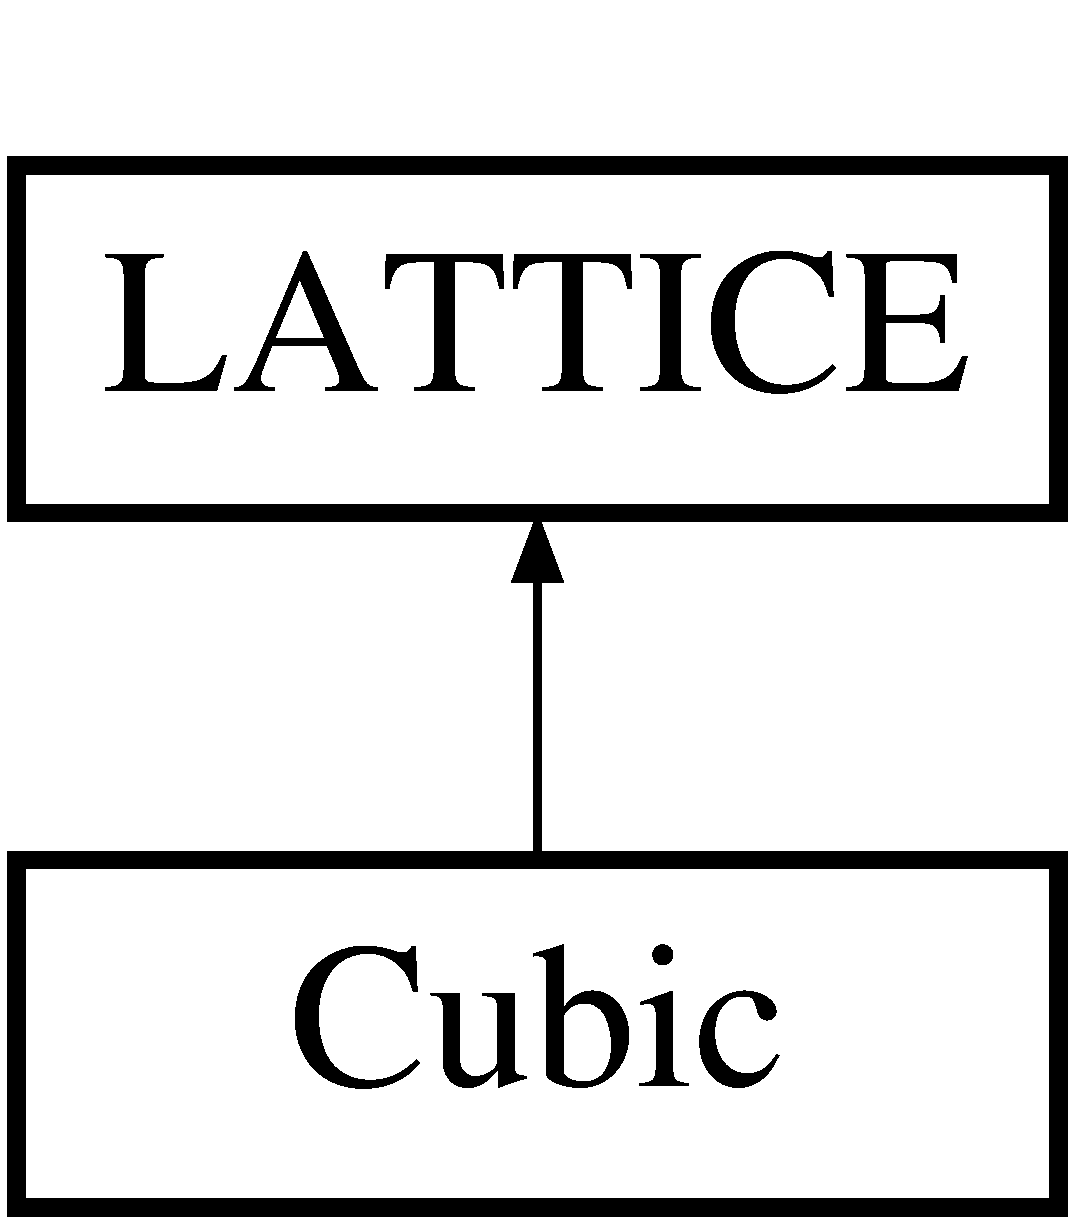
\includegraphics[height=2.000000cm]{class_cubic}
\end{center}
\end{figure}
\subsection*{Public Member Functions}
\begin{DoxyCompactItemize}
\item 
\hyperlink{class_cubic_a6623f1c4fa208bcb35e0ff739fe4f8ef}{Cubic} (double i\+\_\+alat, char i\+\_\+lstyle\mbox{[}$\,$\mbox{]}, char $\ast$i\+\_\+element)
\begin{DoxyCompactList}\small\item\em Constructor for the \hyperlink{class_cubic}{Cubic} Bravais class when accessed from a gui session or when reading a parameters file. \end{DoxyCompactList}\item 
\hyperlink{class_cubic_ad2d13776cf53d7681dcfb1a9feb72116}{$\sim$\+Cubic} ()
\end{DoxyCompactItemize}
\subsection*{Private Member Functions}
\begin{DoxyCompactItemize}
\item 
void \hyperlink{class_cubic_ac7c7d6cb6f96269df131cbe0c2ecb42e}{primitive} ()
\begin{DoxyCompactList}\small\item\em Defines lattice vectors, lattice parameters, and basis atoms for Simple \hyperlink{class_cubic}{Cubic}. \end{DoxyCompactList}\item 
void \hyperlink{class_cubic_ae8cc04295829b5f58eb90207bce4b83b}{B\+C\+C} ()
\begin{DoxyCompactList}\small\item\em Defines lattice vectors, lattice parameters, and basis atoms for Body Centered \hyperlink{class_cubic}{Cubic}. \end{DoxyCompactList}\item 
void \hyperlink{class_cubic_a699d8d8aec47dc6a32b05543024f1f3c}{F\+C\+C} ()
\begin{DoxyCompactList}\small\item\em Defines lattice vectors, lattice parameters, and basis atoms for Face Centered \hyperlink{class_cubic}{Cubic}. \end{DoxyCompactList}\item 
void \hyperlink{class_cubic_ad98a7df81bbf23d7d337a870e709bbc9}{Diamond} ()
\begin{DoxyCompactList}\small\item\em Defines lattice vectors, lattice parameters, and basis atoms for Diamond. \end{DoxyCompactList}\end{DoxyCompactItemize}
\subsection*{Additional Inherited Members}


\subsection{Constructor \& Destructor Documentation}
\hypertarget{class_cubic_a6623f1c4fa208bcb35e0ff739fe4f8ef}{}\index{Cubic@{Cubic}!Cubic@{Cubic}}
\index{Cubic@{Cubic}!Cubic@{Cubic}}
\subsubsection[{Cubic}]{\setlength{\rightskip}{0pt plus 5cm}Cubic\+::\+Cubic (
\begin{DoxyParamCaption}
\item[{double}]{i\+\_\+alat, }
\item[{char}]{i\+\_\+lstyle\mbox{[}$\,$\mbox{]}, }
\item[{char $\ast$}]{i\+\_\+element}
\end{DoxyParamCaption}
)}\label{class_cubic_a6623f1c4fa208bcb35e0ff739fe4f8ef}


Constructor for the \hyperlink{class_cubic}{Cubic} Bravais class when accessed from a gui session or when reading a parameters file. 


\begin{DoxyParams}[1]{Parameters}
\mbox{\tt in}  & {\em i\+\_\+alat} & -\/ lattice parameter for {\ttfamily a}, in Å \\
\hline
\mbox{\tt in}  & {\em i\+\_\+lstyle} & -\/ which cubic crystal style, \begin{DoxyItemize}
\item {\ttfamily S\+C}, {\ttfamily B\+C\+C}, {\ttfamily F\+C\+C}, {\ttfamily Diamond} \end{DoxyItemize}
\\
\hline
\mbox{\tt in}  & {\em i\+\_\+element} & -\/ which element to assign to the crystal \\
\hline
\end{DoxyParams}
\hypertarget{class_cubic_ad2d13776cf53d7681dcfb1a9feb72116}{}\index{Cubic@{Cubic}!````~Cubic@{$\sim$\+Cubic}}
\index{````~Cubic@{$\sim$\+Cubic}!Cubic@{Cubic}}
\subsubsection[{$\sim$\+Cubic}]{\setlength{\rightskip}{0pt plus 5cm}Cubic\+::$\sim$\+Cubic (
\begin{DoxyParamCaption}
{}
\end{DoxyParamCaption}
)}\label{class_cubic_ad2d13776cf53d7681dcfb1a9feb72116}


\subsection{Member Function Documentation}
\hypertarget{class_cubic_ae8cc04295829b5f58eb90207bce4b83b}{}\index{Cubic@{Cubic}!B\+C\+C@{B\+C\+C}}
\index{B\+C\+C@{B\+C\+C}!Cubic@{Cubic}}
\subsubsection[{B\+C\+C}]{\setlength{\rightskip}{0pt plus 5cm}void Cubic\+::\+B\+C\+C (
\begin{DoxyParamCaption}
{}
\end{DoxyParamCaption}
)\hspace{0.3cm}{\ttfamily [private]}}\label{class_cubic_ae8cc04295829b5f58eb90207bce4b83b}


Defines lattice vectors, lattice parameters, and basis atoms for Body Centered \hyperlink{class_cubic}{Cubic}. 

\hypertarget{class_cubic_ad98a7df81bbf23d7d337a870e709bbc9}{}\index{Cubic@{Cubic}!Diamond@{Diamond}}
\index{Diamond@{Diamond}!Cubic@{Cubic}}
\subsubsection[{Diamond}]{\setlength{\rightskip}{0pt plus 5cm}void Cubic\+::\+Diamond (
\begin{DoxyParamCaption}
{}
\end{DoxyParamCaption}
)\hspace{0.3cm}{\ttfamily [private]}}\label{class_cubic_ad98a7df81bbf23d7d337a870e709bbc9}


Defines lattice vectors, lattice parameters, and basis atoms for Diamond. 

\hypertarget{class_cubic_a699d8d8aec47dc6a32b05543024f1f3c}{}\index{Cubic@{Cubic}!F\+C\+C@{F\+C\+C}}
\index{F\+C\+C@{F\+C\+C}!Cubic@{Cubic}}
\subsubsection[{F\+C\+C}]{\setlength{\rightskip}{0pt plus 5cm}void Cubic\+::\+F\+C\+C (
\begin{DoxyParamCaption}
{}
\end{DoxyParamCaption}
)\hspace{0.3cm}{\ttfamily [private]}}\label{class_cubic_a699d8d8aec47dc6a32b05543024f1f3c}


Defines lattice vectors, lattice parameters, and basis atoms for Face Centered \hyperlink{class_cubic}{Cubic}. 

\hypertarget{class_cubic_ac7c7d6cb6f96269df131cbe0c2ecb42e}{}\index{Cubic@{Cubic}!primitive@{primitive}}
\index{primitive@{primitive}!Cubic@{Cubic}}
\subsubsection[{primitive}]{\setlength{\rightskip}{0pt plus 5cm}void Cubic\+::primitive (
\begin{DoxyParamCaption}
{}
\end{DoxyParamCaption}
)\hspace{0.3cm}{\ttfamily [private]}}\label{class_cubic_ac7c7d6cb6f96269df131cbe0c2ecb42e}


Defines lattice vectors, lattice parameters, and basis atoms for Simple \hyperlink{class_cubic}{Cubic}. 



The documentation for this class was generated from the following file\+:\begin{DoxyCompactItemize}
\item 
src/structures/\hyperlink{cubic_8h}{cubic.\+h}\end{DoxyCompactItemize}

\hypertarget{class_custom}{}\section{Custom Class Reference}
\label{class_custom}\index{Custom@{Custom}}


\subsection{Detailed Description}
\subsection*{{\bfseries Purpose\+:} }

\begin{DoxyVerb}/***************************************************************************************\
/  Class to create a custom lattice from scratch by specifying the lattice              \
/  parameters, (a, b, c) and the lattice angles (α, β, γ )                              \
/  Additionally, the basis can be defined on the fly with any number of                 \
/  atomic species within the unit cell.  The basis coordinates are assumed              \
/  to be in fractional units, and in the correct stoichiometric order,                  \
/  i.e. PETN = C10 H16 8N 24O ==> 1-11 basis atoms to C, 12-28 basis atoms to H, etc..  \
/                                                                                       \ 
/  The orientation of the crystal is such that a1 is colinear with the x-axis.          \
/  a2 is obtained by rotating a1 by γ about the z-axis                                  \
/  a3 is obtained by rotating a1 by -β about the y-axis                                 \
/***************************************************************************************\
\end{DoxyVerb}


\begin{DoxyAuthor}{Author}
Joseph M. Gonzalez
\end{DoxyAuthor}
\begin{DoxyVersion}{Version}
0.\+1
\end{DoxyVersion}
\begin{DoxyDate}{Date}
Sep 20, 2015 15\+:16\+:20
\end{DoxyDate}
{\bfseries Contact} ~\newline
 \href{mailto:jmgonza6@mail.usf.edu}{\tt jmgonza6@mail.\+usf.\+edu} Inheritance diagram for Custom\+:\begin{figure}[H]
\begin{center}
\leavevmode
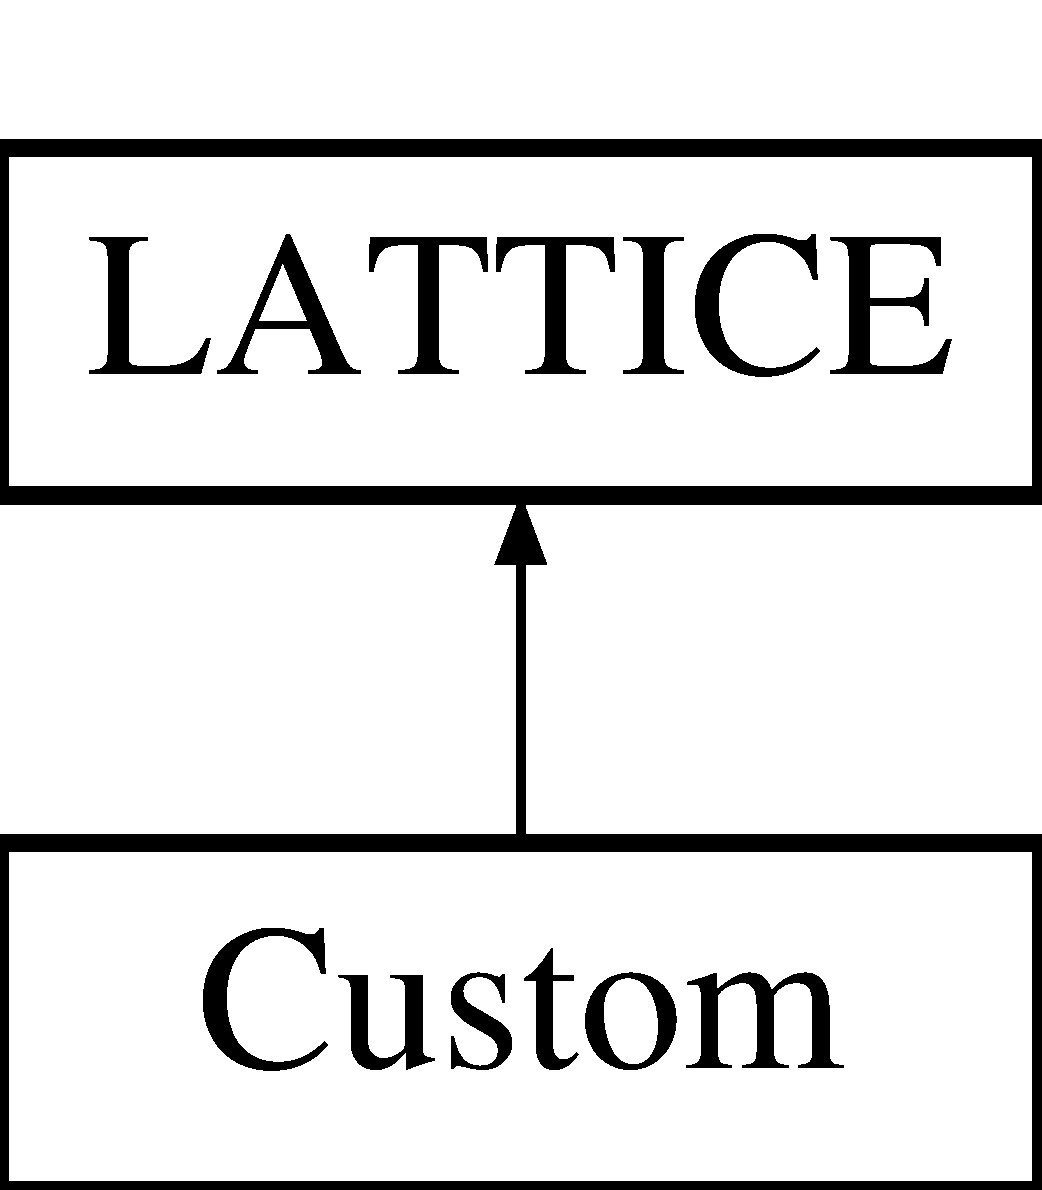
\includegraphics[height=2.000000cm]{class_custom}
\end{center}
\end{figure}
\subsection*{Public Member Functions}
\begin{DoxyCompactItemize}
\item 
\hyperlink{class_custom_a2c066c0d5c4a88a24f3442a173b8f460}{Custom} (double lat\+Pars\mbox{[}3\mbox{]}, double lat\+Angles\mbox{[}3\mbox{]}, std\+::vector$<$ std\+::vector$<$ double $>$ $>$ positions, std\+::string custom\+Name, std\+::vector$<$ std\+::string $>$ elem\+List, std\+::vector$<$ int $>$ \hyperlink{class_l_a_t_t_i_c_e_a63bb555fee4e3cc086f0826437aa5af8}{elem\+Count})
\begin{DoxyCompactList}\small\item\em Constructor for creating a custom crystal when accessed from a gui session or when reading a parameters file. \end{DoxyCompactList}\item 
\hyperlink{class_custom_a7e649363f16d1607a4c62d9bb3747b07}{$\sim$\+Custom} ()
\end{DoxyCompactItemize}
\subsection*{Additional Inherited Members}


\subsection{Constructor \& Destructor Documentation}
\hypertarget{class_custom_a2c066c0d5c4a88a24f3442a173b8f460}{}\index{Custom@{Custom}!Custom@{Custom}}
\index{Custom@{Custom}!Custom@{Custom}}
\subsubsection[{Custom}]{\setlength{\rightskip}{0pt plus 5cm}Custom\+::\+Custom (
\begin{DoxyParamCaption}
\item[{double}]{lat\+Pars\mbox{[}3\mbox{]}, }
\item[{double}]{lat\+Angles\mbox{[}3\mbox{]}, }
\item[{std\+::vector$<$ std\+::vector$<$ double $>$ $>$}]{positions, }
\item[{std\+::string}]{custom\+Name, }
\item[{std\+::vector$<$ std\+::string $>$}]{elem\+List, }
\item[{std\+::vector$<$ int $>$}]{elem\+Count}
\end{DoxyParamCaption}
)}\label{class_custom_a2c066c0d5c4a88a24f3442a173b8f460}


Constructor for creating a custom crystal when accessed from a gui session or when reading a parameters file. 


\begin{DoxyParams}[1]{Parameters}
\mbox{\tt in}  & {\em lat\+Pars} & -\/ array containing the lattice parameters in (Å) \begin{DoxyItemize}
\item lat\+Pars\mbox{[}0\mbox{]} = {\ttfamily a}, \item lat\+Pars\mbox{[}1\mbox{]} = {\ttfamily b}, \item lat\+Pars\mbox{[}2\mbox{]} = {\ttfamily c} \end{DoxyItemize}
\\
\hline
\mbox{\tt in}  & {\em lat\+Angles} & -\/ array containing the lattice angles in (˚) \begin{DoxyItemize}
\item lat\+Angles\mbox{[}0\mbox{]} = {\ttfamily α}, \item lat\+Angles\mbox{[}1\mbox{]} = {\ttfamily β}, \item lat\+Angles\mbox{[}2\mbox{]} = {\ttfamily γ} \end{DoxyItemize}
\\
\hline
\mbox{\tt in}  & {\em positions} & -\/ basis atom positions \\
\hline
\mbox{\tt in}  & {\em custom\+Name} & -\/ name given to the custom lattice, currently this is the formula unit, i.\+e. Mo\+S2 \\
\hline
\mbox{\tt in}  & {\em elem\+List} & -\/ list of the atomic species specified by the user \\
\hline
\mbox{\tt in}  & {\em elem\+Count} & -\/ list containing the stoichiometric coefficients for elements in {\ttfamily elem\+List} \\
\hline
\end{DoxyParams}
\hypertarget{class_custom_a7e649363f16d1607a4c62d9bb3747b07}{}\index{Custom@{Custom}!````~Custom@{$\sim$\+Custom}}
\index{````~Custom@{$\sim$\+Custom}!Custom@{Custom}}
\subsubsection[{$\sim$\+Custom}]{\setlength{\rightskip}{0pt plus 5cm}Custom\+::$\sim$\+Custom (
\begin{DoxyParamCaption}
{}
\end{DoxyParamCaption}
)}\label{class_custom_a7e649363f16d1607a4c62d9bb3747b07}


The documentation for this class was generated from the following file\+:\begin{DoxyCompactItemize}
\item 
src/structures/\hyperlink{custom_8h}{custom.\+h}\end{DoxyCompactItemize}

\hypertarget{class_errors}{}\section{Errors Class Reference}
\label{class_errors}\index{Errors@{Errors}}


\subsection{Detailed Description}
\subsection*{{\bfseries Purpose\+:} }

\begin{DoxyVerb}/*****************************************************************************\
/  Class to process different types of warnings, errors and usage info        \
/                                                                             \
/*****************************************************************************\
\end{DoxyVerb}


\begin{DoxyAuthor}{Author}
Joseph M. Gonzalez
\end{DoxyAuthor}
\begin{DoxyVersion}{Version}
0.\+1
\end{DoxyVersion}
\begin{DoxyDate}{Date}
Sep 13, 2015 19\+:16\+:20
\end{DoxyDate}
{\bfseries Contact} ~\newline
 \href{mailto:jmgonza6@mail.usf.edu}{\tt jmgonza6@mail.\+usf.\+edu} \subsection*{Public Member Functions}
\begin{DoxyCompactItemize}
\item 
\hyperlink{class_errors_aa266bfe6d658cd3e169b18277b902e56}{Errors} ()
\item 
\hyperlink{class_errors_ae7e127294d7af8814b4141eb82cdf80e}{$\sim$\+Errors} ()
\item 
void \hyperlink{class_errors_a7edc156cbfe343a26fbae1d6f6bdd215}{kill} (const char $\ast$file, const char $\ast$subroutine, int line, const char $\ast$message)
\begin{DoxyCompactList}\small\item\em Throw a fatal error and kill the entire run. \end{DoxyCompactList}\item 
void \hyperlink{class_errors_a7f4042d6992ae40907919a2494cf2c80}{warn} (const char $\ast$file, const char $\ast$subroutine, int line, const char $\ast$message)
\begin{DoxyCompactList}\small\item\em Throw a warning, print a message and continue on. \end{DoxyCompactList}\item 
void \hyperlink{class_errors_a3fbf3565c28224fe193828677cb8a277}{show\+\_\+usage\+\_\+info} (const char $\ast$func\+Name)
\begin{DoxyCompactList}\small\item\em Show a list of the possible parameters and operational modes of the program. \end{DoxyCompactList}\end{DoxyCompactItemize}


\subsection{Constructor \& Destructor Documentation}
\hypertarget{class_errors_aa266bfe6d658cd3e169b18277b902e56}{}\index{Errors@{Errors}!Errors@{Errors}}
\index{Errors@{Errors}!Errors@{Errors}}
\subsubsection[{Errors}]{\setlength{\rightskip}{0pt plus 5cm}Errors\+::\+Errors (
\begin{DoxyParamCaption}
{}
\end{DoxyParamCaption}
)}\label{class_errors_aa266bfe6d658cd3e169b18277b902e56}
\hypertarget{class_errors_ae7e127294d7af8814b4141eb82cdf80e}{}\index{Errors@{Errors}!````~Errors@{$\sim$\+Errors}}
\index{````~Errors@{$\sim$\+Errors}!Errors@{Errors}}
\subsubsection[{$\sim$\+Errors}]{\setlength{\rightskip}{0pt plus 5cm}Errors\+::$\sim$\+Errors (
\begin{DoxyParamCaption}
{}
\end{DoxyParamCaption}
)}\label{class_errors_ae7e127294d7af8814b4141eb82cdf80e}


\subsection{Member Function Documentation}
\hypertarget{class_errors_a7edc156cbfe343a26fbae1d6f6bdd215}{}\index{Errors@{Errors}!kill@{kill}}
\index{kill@{kill}!Errors@{Errors}}
\subsubsection[{kill}]{\setlength{\rightskip}{0pt plus 5cm}void Errors\+::kill (
\begin{DoxyParamCaption}
\item[{const char $\ast$}]{file, }
\item[{const char $\ast$}]{subroutine, }
\item[{int}]{line, }
\item[{const char $\ast$}]{message}
\end{DoxyParamCaption}
)}\label{class_errors_a7edc156cbfe343a26fbae1d6f6bdd215}


Throw a fatal error and kill the entire run. 


\begin{DoxyParams}{Parameters}
{\em file} & -\/ file in which error occured \\
\hline
{\em subroutine} & -\/ subroutine throwing the error \\
\hline
{\em line} & -\/ line on which the error occured \\
\hline
{\em message} & -\/ message to the user with the details of the error \\
\hline
\end{DoxyParams}
\hypertarget{class_errors_a3fbf3565c28224fe193828677cb8a277}{}\index{Errors@{Errors}!show\+\_\+usage\+\_\+info@{show\+\_\+usage\+\_\+info}}
\index{show\+\_\+usage\+\_\+info@{show\+\_\+usage\+\_\+info}!Errors@{Errors}}
\subsubsection[{show\+\_\+usage\+\_\+info}]{\setlength{\rightskip}{0pt plus 5cm}void Errors\+::show\+\_\+usage\+\_\+info (
\begin{DoxyParamCaption}
\item[{const char $\ast$}]{func\+Name}
\end{DoxyParamCaption}
)}\label{class_errors_a3fbf3565c28224fe193828677cb8a277}


Show a list of the possible parameters and operational modes of the program. 


\begin{DoxyParams}{Parameters}
{\em func\+Name} & -\/ name of the calling function \\
\hline
\end{DoxyParams}
\hypertarget{class_errors_a7f4042d6992ae40907919a2494cf2c80}{}\index{Errors@{Errors}!warn@{warn}}
\index{warn@{warn}!Errors@{Errors}}
\subsubsection[{warn}]{\setlength{\rightskip}{0pt plus 5cm}void Errors\+::warn (
\begin{DoxyParamCaption}
\item[{const char $\ast$}]{file, }
\item[{const char $\ast$}]{subroutine, }
\item[{int}]{line, }
\item[{const char $\ast$}]{message}
\end{DoxyParamCaption}
)}\label{class_errors_a7f4042d6992ae40907919a2494cf2c80}


Throw a warning, print a message and continue on. 


\begin{DoxyParams}{Parameters}
{\em file} & -\/ file in which warning occured \\
\hline
{\em subroutine} & -\/ subroutine throwing the warning \\
\hline
{\em line} & -\/ line on which the warning occured \\
\hline
{\em message} & -\/ message to the user with the details of the warning \\
\hline
\end{DoxyParams}


The documentation for this class was generated from the following file\+:\begin{DoxyCompactItemize}
\item 
src/util/\hyperlink{common_8h}{common.\+h}\end{DoxyCompactItemize}

\hypertarget{class_gui}{}\section{Gui Class Reference}
\label{class_gui}\index{Gui@{Gui}}


\subsection{Detailed Description}
\subsection*{{\bfseries Purpose\+:} }

\begin{DoxyVerb}/*****************************************************************************\
/  Class which initializes, displays, and monitors all activity in the GUI    \
/                                                                             \
/*****************************************************************************\
\end{DoxyVerb}


\begin{DoxyAuthor}{Author}
Joseph M. Gonzalez
\end{DoxyAuthor}
\begin{DoxyVersion}{Version}
0.\+9
\end{DoxyVersion}
\begin{DoxyDate}{Date}
Sep 13, 2015 19\+:16\+:20
\end{DoxyDate}
{\bfseries Contact} ~\newline
 \href{mailto:jmgonza6@mail.usf.edu}{\tt jmgonza6@mail.\+usf.\+edu} \subsection*{Public Member Functions}
\begin{DoxyCompactItemize}
\item 
\hyperlink{class_gui_ab2655dbb6d3a91d7e90cb83dad6c0450}{Gui} ()
\begin{DoxyCompactList}\small\item\em Constructor launches an instances of the parser class to handle the string maniupulations. It also defines all of the global variables to a reasonable value so that the app can be run with as little interaction as possible. \end{DoxyCompactList}\item 
\hyperlink{class_gui_a4fd8485d226f9b8a2ac2d81d7f0f3598}{$\sim$\+Gui} ()
\item 
void \hyperlink{class_gui_a4fa5f2bbb698866797f66f002627aae0}{display\+\_\+in} (Gtk\+Widget $\ast$window)
\begin{DoxyCompactList}\small\item\em Initialize the G\+T\+K environment and define layout of the gui. creates a notebook style gui with 4 main tabs and 4 buttons for rendering, building, reseting, and exiting. \end{DoxyCompactList}\item 
void \hyperlink{class_gui_a1c73249d03432a2fedd220c0b8c9269b}{save\+\_\+settings} ()
\begin{DoxyCompactList}\small\item\em Store the global variables set by the callback functions layout of the gui. \end{DoxyCompactList}\end{DoxyCompactItemize}
\subsection*{Data Fields}
\begin{DoxyCompactItemize}
\item 
double \hyperlink{class_gui_a1f0bf13bd26f8dbb3756f4475d50ea3b}{alat}
\begin{DoxyCompactList}\small\item\em latttice parameter a (Å) \end{DoxyCompactList}\item 
double \hyperlink{class_gui_a2bf9af74005d7da17b63c00328831fd3}{blat}
\begin{DoxyCompactList}\small\item\em lattice parameter b (Å) \end{DoxyCompactList}\item 
double \hyperlink{class_gui_ac92e0603324d6b978d1813d0d0c2bef9}{clat}
\begin{DoxyCompactList}\small\item\em lattice parameter c (Å) \end{DoxyCompactList}\item 
double \hyperlink{class_gui_af21a8a5ef3954775896ef3ebc4f12ec5}{alpha}
\begin{DoxyCompactList}\small\item\em angle beteween c \& b \end{DoxyCompactList}\item 
double \hyperlink{class_gui_a2b89466ec45a283f6d7b94b6ffc36640}{beta}
\begin{DoxyCompactList}\small\item\em angle between c \& a \end{DoxyCompactList}\item 
double \hyperlink{class_gui_abe1f84fa6c83a5b3b0d939e6be73d3b5}{gamma}
\begin{DoxyCompactList}\small\item\em angle between a \& b \end{DoxyCompactList}\item 
double \hyperlink{class_gui_a105eb1ab34dee685c11005e47c44ee16}{cta}
\begin{DoxyCompactList}\small\item\em c/a ratio, for use with Hexagonal(), h-\/\+B\+N(), Graphene() \end{DoxyCompactList}\item 
int \hyperlink{class_gui_a8c9eebe2e978c4d0bc1bef77905c7738}{lbasis}
\begin{DoxyCompactList}\small\item\em number of basis atoms for graphene \end{DoxyCompactList}\item 
int \hyperlink{class_gui_a6cb804a1531c51117e44674f83a3fbed}{nx}
\begin{DoxyCompactList}\small\item\em supercell dimension along x \end{DoxyCompactList}\item 
int \hyperlink{class_gui_a6a052cca0478f86e3c80535db522fe0a}{ny}
\begin{DoxyCompactList}\small\item\em supercell dimension along y \end{DoxyCompactList}\item 
int \hyperlink{class_gui_aa2511bfa549615e75150f6e5fe81b5c0}{nz}
\begin{DoxyCompactList}\small\item\em supercell dimension along z \end{DoxyCompactList}\item 
int \hyperlink{class_gui_a7b7337d99ba2860adbe3ab2e48d35338}{fractional}
\begin{DoxyCompactList}\small\item\em fractional coordinates, 1 = true, 0 = false \end{DoxyCompactList}\item 
int \hyperlink{class_gui_ae0e6f586344389900c55dc4eaa5206db}{graphene}
\begin{DoxyCompactList}\small\item\em graphene structure was built, 1 = true, 0 = false \end{DoxyCompactList}\item 
int \hyperlink{class_gui_aedb074749fe28d1c9b11b5200017b1a7}{custom}
\begin{DoxyCompactList}\small\item\em a custom structure was built, 1 = true, 0 = false \end{DoxyCompactList}\item 
int \hyperlink{class_gui_a45506f3be90d2d61d0ec66205384e823}{resets}
\begin{DoxyCompactList}\small\item\em reset count \end{DoxyCompactList}\item 
int \hyperlink{class_gui_a4140b79a0f551c7650ecb3a2571c1e83}{run\+\_\+count}
\begin{DoxyCompactList}\small\item\em run count, for debugging \end{DoxyCompactList}\item 
int \hyperlink{class_gui_a218cd4709b84a4aa7110bbf43e050c3c}{quit}
\begin{DoxyCompactList}\small\item\em quit signal \end{DoxyCompactList}\item 
int \hyperlink{class_gui_a0ad7bdad878125b0c6a08949e572e109}{view}
\begin{DoxyCompactList}\small\item\em render+build signal \end{DoxyCompactList}\item 
char $\ast$ \hyperlink{class_gui_ad78f3255742971f001f7c509c66ff655}{pfile}
\begin{DoxyCompactList}\small\item\em parameter file to define the crystal \end{DoxyCompactList}\item 
char $\ast$ \hyperlink{class_gui_a29e73c724fb7465a012847876688c405}{out\+\_\+name}
\begin{DoxyCompactList}\small\item\em file name to write \end{DoxyCompactList}\item 
char $\ast$ \hyperlink{class_gui_afe858ad21a3a036632416f887fe06d37}{file\+\_\+format}
\begin{DoxyCompactList}\small\item\em type of file to write \end{DoxyCompactList}\item 
char $\ast$ \hyperlink{class_gui_afeba585e007765820c01f71e7b5f7c87}{bravais}
\begin{DoxyCompactList}\small\item\em which lattice ? \end{DoxyCompactList}\item 
char $\ast$ \hyperlink{class_gui_a39bb625a90cea3d763c46bb68e87ab11}{lstyle}
\begin{DoxyCompactList}\small\item\em bravais lattice style, B\+C\+C \end{DoxyCompactList}\item 
char $\ast$ \hyperlink{class_gui_ad256ded075bfb167743bb388ec301fe4}{pd\+\_\+struct}
\begin{DoxyCompactList}\small\item\em defines a library structure to use \end{DoxyCompactList}\item 
char $\ast$ \hyperlink{class_gui_a2cb3d0d19735c9b7c0acaab6a236eb17}{element}
\begin{DoxyCompactList}\small\item\em which species ? \end{DoxyCompactList}\item 
std\+::vector$<$ std\+::string $>$ \hyperlink{class_gui_a33f327cf44f8231253a244d582cc7a9c}{elem\+List}
\begin{DoxyCompactList}\small\item\em define a custom stoichiometry (C,H,N,O) \end{DoxyCompactList}\item 
std\+::vector$<$ int $>$ \hyperlink{class_gui_af3e1a1fb1647e26d6a8a41e051d7433b}{elem\+Count}
\begin{DoxyCompactList}\small\item\em define a custom stoichiometry (2,4,1,3) \end{DoxyCompactList}\item 
std\+::vector$<$ std\+::vector$<$ double $>$ $>$ \hyperlink{class_gui_a0ba23b6cdb6a13e279ebb07098e265b5}{custom\+Basis}
\begin{DoxyCompactList}\small\item\em container for defining a custom basis set \end{DoxyCompactList}\item 
std\+::string \hyperlink{class_gui_a062cae171eaf8234689de5fe473692e3}{custom\+Name}
\begin{DoxyCompactList}\small\item\em chemical formula of a custom structure \end{DoxyCompactList}\end{DoxyCompactItemize}
\subsection*{Private Member Functions}
\begin{DoxyCompactItemize}
\item 
Gtk\+Widget $\ast$ \hyperlink{class_gui_aee0db69625943019e5a9b99ba22c0348}{fill\+\_\+dropdown} (const char $\ast$style)
\item 
void \hyperlink{class_gui_a6286dfbea72f91549c5af39c8a2ccc86}{define\+\_\+basis\+\_\+atoms} ()
\end{DoxyCompactItemize}
\subsection*{Static Private Member Functions}
\begin{DoxyCompactItemize}
\item 
static void \hyperlink{class_gui_a0361446932ea24631a9a309ecd4918e2}{open\+\_\+browser} (Gtk\+Widget $\ast$button, gpointer window)
\item 
static void \hyperlink{class_gui_a96dd2566bc45f990c6b8ab59d1344153}{save\+\_\+browser} (Gtk\+Widget $\ast$button, gpointer window)
\item 
static void \hyperlink{class_gui_a7d50ca2f38ae76e0cfd9444651542d4b}{build\+\_\+crystal} (Gtk\+Widget $\ast$button, gpointer window)
\item 
static void \hyperlink{class_gui_a640296a9a21d37a07e963ff3eb6d3590}{reset\+\_\+parameters} (Gtk\+Widget $\ast$button, gpointer window)
\item 
static void \hyperlink{class_gui_abe49e057b7c93c1432a20a7ed57fcbdf}{open\+\_\+dialog} (const char $\ast$syst, char message\mbox{[}\hyperlink{common_8h_a6789ebc0df71a8ef76bfbb4fb5f74aad}{M\+A\+X\+\_\+\+S\+T\+R\+I\+N\+G\+\_\+\+L\+E\+N\+G\+T\+H}\mbox{]})
\item 
static void \hyperlink{class_gui_a37d0bad8546197105edfa23a2e6f42ae}{reminder} ()
\item 
static void \hyperlink{class_gui_a95855da00553d4523403a6bfd58e49ac}{graphene\+\_\+dialog} ()
\item 
static void \hyperlink{class_gui_a4232273b39d2b5b3e7a7fdad6a0fc37e}{structures\+\_\+dialog} ()
\item 
static void \hyperlink{class_gui_ab85fa47609a7b87c756fe6c2ebc1c199}{set\+\_\+nx} (Gtk\+Widget $\ast$entry, gpointer data)
\item 
static void \hyperlink{class_gui_a9f0033b84bcee926322da0abf7e9ee16}{set\+\_\+ny} (Gtk\+Widget $\ast$entry, gpointer data)
\item 
static void \hyperlink{class_gui_a3fc8d99c08f107497b8ab3ef312fe60b}{set\+\_\+nz} (Gtk\+Widget $\ast$entry, gpointer data)
\item 
static void \hyperlink{class_gui_a6e21579571ee32042c0723818da76faa}{set\+\_\+atom\+\_\+species} (Gtk\+Combo\+Box $\ast$dropdown, gpointer data)
\item 
static void \hyperlink{class_gui_abf2197f1d93849923cb63de803478b87}{set\+\_\+write\+\_\+style} (Gtk\+Combo\+Box $\ast$dropdown, gpointer data)
\item 
static void \hyperlink{class_gui_a1143cda5695a043bb2a4f071f1cded77}{set\+\_\+bravais} (Gtk\+Combo\+Box $\ast$dropdown, gpointer data)
\item 
static void \hyperlink{class_gui_a05621e2bb9936636caf3128d1611827a}{set\+\_\+lattice\+\_\+style} (Gtk\+Combo\+Box $\ast$widget, gpointer data)
\item 
static void \hyperlink{class_gui_a334a7a04a6c00f24abddfa94de8f10ce}{quit\+\_\+main} (Gtk\+Widget $\ast$widget, gpointer data)
\item 
static void \hyperlink{class_gui_aa8edfa548ee3ebcb325c43086b196fe0}{render\+\_\+crystal} (Gtk\+Widget $\ast$widget, gpointer data)
\item 
static void \hyperlink{class_gui_a61dd19b2b81db0839543802814d7f49e}{set\+\_\+pd\+\_\+struct} (Gtk\+Combo\+Box $\ast$dropdown, gpointer data)
\item 
static void \hyperlink{class_gui_af78ce4976f95571adaf5260fe140337d}{set\+\_\+custom\+\_\+species} (Gtk\+Widget $\ast$entry, gpointer data)
\item 
static void \hyperlink{class_gui_a2ef155d1b6279e72dabdb2ce0fa03e59}{set\+\_\+alat} (Gtk\+Widget $\ast$entry, gpointer data)
\item 
static void \hyperlink{class_gui_abd57037f5c09c0ea7f20264fbdd630ca}{set\+\_\+blat} (Gtk\+Widget $\ast$entry, gpointer data)
\item 
static void \hyperlink{class_gui_aada6cadb96bb3b486efa192e5e5f8b51}{set\+\_\+clat} (Gtk\+Widget $\ast$entry, gpointer data)
\item 
static void \hyperlink{class_gui_a4e7013cc9f0d4bbe495311fc94643342}{set\+\_\+alpha} (Gtk\+Widget $\ast$entry, gpointer data)
\item 
static void \hyperlink{class_gui_ad4cb1cb7fb9df0a9681ab4f90f47561f}{set\+\_\+beta} (Gtk\+Widget $\ast$entry, gpointer data)
\item 
static void \hyperlink{class_gui_a453aa0ae8fc7a1563c77af6210e31385}{set\+\_\+gamma} (Gtk\+Widget $\ast$entry, gpointer data)
\item 
static void \hyperlink{class_gui_a0a5d7e785101e584a6c1e5bfd6dc3fd0}{set\+\_\+graphene\+\_\+basis} (Gtk\+Widget $\ast$entry, gpointer data)
\item 
static void \hyperlink{class_gui_a09d25819dce6dfe57c3204778394b3b9}{set\+\_\+cta} (Gtk\+Widget $\ast$entry, gpointer data)
\item 
static void \hyperlink{class_gui_ab31975e08d40ee52c8c5ce6f74b983ff}{open\+\_\+advanced} (Gtk\+Widget $\ast$button, gpointer data)
\item 
static void \hyperlink{class_gui_ae2f11430530160cca5130c585edc03a1}{set\+\_\+fract} (Gtk\+Toggle\+Button $\ast$swtch)
\item 
static void \hyperlink{class_gui_a7ce7c501381dbdc948ccb2bec0b47284}{set\+\_\+cart} (Gtk\+Toggle\+Button $\ast$swtch)
\item 
static void \hyperlink{class_gui_a2d7195079aac03f9c62e0dc78c01eec9}{add\+\_\+atom\+\_\+window} (Gtk\+Widget $\ast$widget, gpointer data)
\item 
static void \hyperlink{class_gui_aa44e21bc4f18f1815d6ddf5c7b42a089}{add\+\_\+atom} (Gtk\+Widget $\ast$entry, gpointer data)
\item 
static void \hyperlink{class_gui_a6a4a9bf6bd478b794f30d22932e8fbe0}{reset\+\_\+basis} (Gtk\+Widget $\ast$widget, gpointer data)
\end{DoxyCompactItemize}
\subsection*{Private Attributes}
\begin{DoxyCompactItemize}
\item 
\hyperlink{class_parser}{Parser} $\ast$ \hyperlink{class_gui_a768d5cc7d6721405061620216159d20d}{parser}
\end{DoxyCompactItemize}


\subsection{Constructor \& Destructor Documentation}
\hypertarget{class_gui_ab2655dbb6d3a91d7e90cb83dad6c0450}{}\index{Gui@{Gui}!Gui@{Gui}}
\index{Gui@{Gui}!Gui@{Gui}}
\subsubsection[{Gui}]{\setlength{\rightskip}{0pt plus 5cm}Gui\+::\+Gui (
\begin{DoxyParamCaption}
{}
\end{DoxyParamCaption}
)}\label{class_gui_ab2655dbb6d3a91d7e90cb83dad6c0450}


Constructor launches an instances of the parser class to handle the string maniupulations. It also defines all of the global variables to a reasonable value so that the app can be run with as little interaction as possible. 

\hypertarget{class_gui_a4fd8485d226f9b8a2ac2d81d7f0f3598}{}\index{Gui@{Gui}!````~Gui@{$\sim$\+Gui}}
\index{````~Gui@{$\sim$\+Gui}!Gui@{Gui}}
\subsubsection[{$\sim$\+Gui}]{\setlength{\rightskip}{0pt plus 5cm}Gui\+::$\sim$\+Gui (
\begin{DoxyParamCaption}
{}
\end{DoxyParamCaption}
)}\label{class_gui_a4fd8485d226f9b8a2ac2d81d7f0f3598}


\subsection{Member Function Documentation}
\hypertarget{class_gui_aa44e21bc4f18f1815d6ddf5c7b42a089}{}\index{Gui@{Gui}!add\+\_\+atom@{add\+\_\+atom}}
\index{add\+\_\+atom@{add\+\_\+atom}!Gui@{Gui}}
\subsubsection[{add\+\_\+atom}]{\setlength{\rightskip}{0pt plus 5cm}static void Gui\+::add\+\_\+atom (
\begin{DoxyParamCaption}
\item[{Gtk\+Widget $\ast$}]{entry, }
\item[{gpointer}]{data}
\end{DoxyParamCaption}
)\hspace{0.3cm}{\ttfamily [static]}, {\ttfamily [private]}}\label{class_gui_aa44e21bc4f18f1815d6ddf5c7b42a089}
\hypertarget{class_gui_a2d7195079aac03f9c62e0dc78c01eec9}{}\index{Gui@{Gui}!add\+\_\+atom\+\_\+window@{add\+\_\+atom\+\_\+window}}
\index{add\+\_\+atom\+\_\+window@{add\+\_\+atom\+\_\+window}!Gui@{Gui}}
\subsubsection[{add\+\_\+atom\+\_\+window}]{\setlength{\rightskip}{0pt plus 5cm}static void Gui\+::add\+\_\+atom\+\_\+window (
\begin{DoxyParamCaption}
\item[{Gtk\+Widget $\ast$}]{widget, }
\item[{gpointer}]{data}
\end{DoxyParamCaption}
)\hspace{0.3cm}{\ttfamily [static]}, {\ttfamily [private]}}\label{class_gui_a2d7195079aac03f9c62e0dc78c01eec9}
\hypertarget{class_gui_a7d50ca2f38ae76e0cfd9444651542d4b}{}\index{Gui@{Gui}!build\+\_\+crystal@{build\+\_\+crystal}}
\index{build\+\_\+crystal@{build\+\_\+crystal}!Gui@{Gui}}
\subsubsection[{build\+\_\+crystal}]{\setlength{\rightskip}{0pt plus 5cm}static void Gui\+::build\+\_\+crystal (
\begin{DoxyParamCaption}
\item[{Gtk\+Widget $\ast$}]{button, }
\item[{gpointer}]{window}
\end{DoxyParamCaption}
)\hspace{0.3cm}{\ttfamily [static]}, {\ttfamily [private]}}\label{class_gui_a7d50ca2f38ae76e0cfd9444651542d4b}
\hypertarget{class_gui_a6286dfbea72f91549c5af39c8a2ccc86}{}\index{Gui@{Gui}!define\+\_\+basis\+\_\+atoms@{define\+\_\+basis\+\_\+atoms}}
\index{define\+\_\+basis\+\_\+atoms@{define\+\_\+basis\+\_\+atoms}!Gui@{Gui}}
\subsubsection[{define\+\_\+basis\+\_\+atoms}]{\setlength{\rightskip}{0pt plus 5cm}void Gui\+::define\+\_\+basis\+\_\+atoms (
\begin{DoxyParamCaption}
{}
\end{DoxyParamCaption}
)\hspace{0.3cm}{\ttfamily [private]}}\label{class_gui_a6286dfbea72f91549c5af39c8a2ccc86}
\hypertarget{class_gui_a4fa5f2bbb698866797f66f002627aae0}{}\index{Gui@{Gui}!display\+\_\+in@{display\+\_\+in}}
\index{display\+\_\+in@{display\+\_\+in}!Gui@{Gui}}
\subsubsection[{display\+\_\+in}]{\setlength{\rightskip}{0pt plus 5cm}void Gui\+::display\+\_\+in (
\begin{DoxyParamCaption}
\item[{Gtk\+Widget $\ast$}]{window}
\end{DoxyParamCaption}
)}\label{class_gui_a4fa5f2bbb698866797f66f002627aae0}


Initialize the G\+T\+K environment and define layout of the gui. creates a notebook style gui with 4 main tabs and 4 buttons for rendering, building, reseting, and exiting. 


\begin{DoxyParams}{Parameters}
{\em window} & -\/ In which window do we create the gui \\
\hline
\end{DoxyParams}
\hypertarget{class_gui_aee0db69625943019e5a9b99ba22c0348}{}\index{Gui@{Gui}!fill\+\_\+dropdown@{fill\+\_\+dropdown}}
\index{fill\+\_\+dropdown@{fill\+\_\+dropdown}!Gui@{Gui}}
\subsubsection[{fill\+\_\+dropdown}]{\setlength{\rightskip}{0pt plus 5cm}Gtk\+Widget$\ast$ Gui\+::fill\+\_\+dropdown (
\begin{DoxyParamCaption}
\item[{const char $\ast$}]{style}
\end{DoxyParamCaption}
)\hspace{0.3cm}{\ttfamily [private]}}\label{class_gui_aee0db69625943019e5a9b99ba22c0348}
\hypertarget{class_gui_a95855da00553d4523403a6bfd58e49ac}{}\index{Gui@{Gui}!graphene\+\_\+dialog@{graphene\+\_\+dialog}}
\index{graphene\+\_\+dialog@{graphene\+\_\+dialog}!Gui@{Gui}}
\subsubsection[{graphene\+\_\+dialog}]{\setlength{\rightskip}{0pt plus 5cm}static void Gui\+::graphene\+\_\+dialog (
\begin{DoxyParamCaption}
{}
\end{DoxyParamCaption}
)\hspace{0.3cm}{\ttfamily [static]}, {\ttfamily [private]}}\label{class_gui_a95855da00553d4523403a6bfd58e49ac}
\hypertarget{class_gui_ab31975e08d40ee52c8c5ce6f74b983ff}{}\index{Gui@{Gui}!open\+\_\+advanced@{open\+\_\+advanced}}
\index{open\+\_\+advanced@{open\+\_\+advanced}!Gui@{Gui}}
\subsubsection[{open\+\_\+advanced}]{\setlength{\rightskip}{0pt plus 5cm}static void Gui\+::open\+\_\+advanced (
\begin{DoxyParamCaption}
\item[{Gtk\+Widget $\ast$}]{button, }
\item[{gpointer}]{data}
\end{DoxyParamCaption}
)\hspace{0.3cm}{\ttfamily [static]}, {\ttfamily [private]}}\label{class_gui_ab31975e08d40ee52c8c5ce6f74b983ff}
\hypertarget{class_gui_a0361446932ea24631a9a309ecd4918e2}{}\index{Gui@{Gui}!open\+\_\+browser@{open\+\_\+browser}}
\index{open\+\_\+browser@{open\+\_\+browser}!Gui@{Gui}}
\subsubsection[{open\+\_\+browser}]{\setlength{\rightskip}{0pt plus 5cm}static void Gui\+::open\+\_\+browser (
\begin{DoxyParamCaption}
\item[{Gtk\+Widget $\ast$}]{button, }
\item[{gpointer}]{window}
\end{DoxyParamCaption}
)\hspace{0.3cm}{\ttfamily [static]}, {\ttfamily [private]}}\label{class_gui_a0361446932ea24631a9a309ecd4918e2}
\hypertarget{class_gui_abe49e057b7c93c1432a20a7ed57fcbdf}{}\index{Gui@{Gui}!open\+\_\+dialog@{open\+\_\+dialog}}
\index{open\+\_\+dialog@{open\+\_\+dialog}!Gui@{Gui}}
\subsubsection[{open\+\_\+dialog}]{\setlength{\rightskip}{0pt plus 5cm}static void Gui\+::open\+\_\+dialog (
\begin{DoxyParamCaption}
\item[{const char $\ast$}]{syst, }
\item[{char}]{message\mbox{[}\+M\+A\+X\+\_\+\+S\+T\+R\+I\+N\+G\+\_\+\+L\+E\+N\+G\+T\+H\mbox{]}}
\end{DoxyParamCaption}
)\hspace{0.3cm}{\ttfamily [static]}, {\ttfamily [private]}}\label{class_gui_abe49e057b7c93c1432a20a7ed57fcbdf}
\hypertarget{class_gui_a334a7a04a6c00f24abddfa94de8f10ce}{}\index{Gui@{Gui}!quit\+\_\+main@{quit\+\_\+main}}
\index{quit\+\_\+main@{quit\+\_\+main}!Gui@{Gui}}
\subsubsection[{quit\+\_\+main}]{\setlength{\rightskip}{0pt plus 5cm}static void Gui\+::quit\+\_\+main (
\begin{DoxyParamCaption}
\item[{Gtk\+Widget $\ast$}]{widget, }
\item[{gpointer}]{data}
\end{DoxyParamCaption}
)\hspace{0.3cm}{\ttfamily [static]}, {\ttfamily [private]}}\label{class_gui_a334a7a04a6c00f24abddfa94de8f10ce}
\hypertarget{class_gui_a37d0bad8546197105edfa23a2e6f42ae}{}\index{Gui@{Gui}!reminder@{reminder}}
\index{reminder@{reminder}!Gui@{Gui}}
\subsubsection[{reminder}]{\setlength{\rightskip}{0pt plus 5cm}static void Gui\+::reminder (
\begin{DoxyParamCaption}
{}
\end{DoxyParamCaption}
)\hspace{0.3cm}{\ttfamily [static]}, {\ttfamily [private]}}\label{class_gui_a37d0bad8546197105edfa23a2e6f42ae}
\hypertarget{class_gui_aa8edfa548ee3ebcb325c43086b196fe0}{}\index{Gui@{Gui}!render\+\_\+crystal@{render\+\_\+crystal}}
\index{render\+\_\+crystal@{render\+\_\+crystal}!Gui@{Gui}}
\subsubsection[{render\+\_\+crystal}]{\setlength{\rightskip}{0pt plus 5cm}static void Gui\+::render\+\_\+crystal (
\begin{DoxyParamCaption}
\item[{Gtk\+Widget $\ast$}]{widget, }
\item[{gpointer}]{data}
\end{DoxyParamCaption}
)\hspace{0.3cm}{\ttfamily [static]}, {\ttfamily [private]}}\label{class_gui_aa8edfa548ee3ebcb325c43086b196fe0}
\hypertarget{class_gui_a6a4a9bf6bd478b794f30d22932e8fbe0}{}\index{Gui@{Gui}!reset\+\_\+basis@{reset\+\_\+basis}}
\index{reset\+\_\+basis@{reset\+\_\+basis}!Gui@{Gui}}
\subsubsection[{reset\+\_\+basis}]{\setlength{\rightskip}{0pt plus 5cm}static void Gui\+::reset\+\_\+basis (
\begin{DoxyParamCaption}
\item[{Gtk\+Widget $\ast$}]{widget, }
\item[{gpointer}]{data}
\end{DoxyParamCaption}
)\hspace{0.3cm}{\ttfamily [static]}, {\ttfamily [private]}}\label{class_gui_a6a4a9bf6bd478b794f30d22932e8fbe0}
\hypertarget{class_gui_a640296a9a21d37a07e963ff3eb6d3590}{}\index{Gui@{Gui}!reset\+\_\+parameters@{reset\+\_\+parameters}}
\index{reset\+\_\+parameters@{reset\+\_\+parameters}!Gui@{Gui}}
\subsubsection[{reset\+\_\+parameters}]{\setlength{\rightskip}{0pt plus 5cm}static void Gui\+::reset\+\_\+parameters (
\begin{DoxyParamCaption}
\item[{Gtk\+Widget $\ast$}]{button, }
\item[{gpointer}]{window}
\end{DoxyParamCaption}
)\hspace{0.3cm}{\ttfamily [static]}, {\ttfamily [private]}}\label{class_gui_a640296a9a21d37a07e963ff3eb6d3590}
\hypertarget{class_gui_a96dd2566bc45f990c6b8ab59d1344153}{}\index{Gui@{Gui}!save\+\_\+browser@{save\+\_\+browser}}
\index{save\+\_\+browser@{save\+\_\+browser}!Gui@{Gui}}
\subsubsection[{save\+\_\+browser}]{\setlength{\rightskip}{0pt plus 5cm}static void Gui\+::save\+\_\+browser (
\begin{DoxyParamCaption}
\item[{Gtk\+Widget $\ast$}]{button, }
\item[{gpointer}]{window}
\end{DoxyParamCaption}
)\hspace{0.3cm}{\ttfamily [static]}, {\ttfamily [private]}}\label{class_gui_a96dd2566bc45f990c6b8ab59d1344153}
\hypertarget{class_gui_a1c73249d03432a2fedd220c0b8c9269b}{}\index{Gui@{Gui}!save\+\_\+settings@{save\+\_\+settings}}
\index{save\+\_\+settings@{save\+\_\+settings}!Gui@{Gui}}
\subsubsection[{save\+\_\+settings}]{\setlength{\rightskip}{0pt plus 5cm}void Gui\+::save\+\_\+settings (
\begin{DoxyParamCaption}
{}
\end{DoxyParamCaption}
)}\label{class_gui_a1c73249d03432a2fedd220c0b8c9269b}


Store the global variables set by the callback functions layout of the gui. 

\hypertarget{class_gui_a2ef155d1b6279e72dabdb2ce0fa03e59}{}\index{Gui@{Gui}!set\+\_\+alat@{set\+\_\+alat}}
\index{set\+\_\+alat@{set\+\_\+alat}!Gui@{Gui}}
\subsubsection[{set\+\_\+alat}]{\setlength{\rightskip}{0pt plus 5cm}static void Gui\+::set\+\_\+alat (
\begin{DoxyParamCaption}
\item[{Gtk\+Widget $\ast$}]{entry, }
\item[{gpointer}]{data}
\end{DoxyParamCaption}
)\hspace{0.3cm}{\ttfamily [static]}, {\ttfamily [private]}}\label{class_gui_a2ef155d1b6279e72dabdb2ce0fa03e59}
\hypertarget{class_gui_a4e7013cc9f0d4bbe495311fc94643342}{}\index{Gui@{Gui}!set\+\_\+alpha@{set\+\_\+alpha}}
\index{set\+\_\+alpha@{set\+\_\+alpha}!Gui@{Gui}}
\subsubsection[{set\+\_\+alpha}]{\setlength{\rightskip}{0pt plus 5cm}static void Gui\+::set\+\_\+alpha (
\begin{DoxyParamCaption}
\item[{Gtk\+Widget $\ast$}]{entry, }
\item[{gpointer}]{data}
\end{DoxyParamCaption}
)\hspace{0.3cm}{\ttfamily [static]}, {\ttfamily [private]}}\label{class_gui_a4e7013cc9f0d4bbe495311fc94643342}
\hypertarget{class_gui_a6e21579571ee32042c0723818da76faa}{}\index{Gui@{Gui}!set\+\_\+atom\+\_\+species@{set\+\_\+atom\+\_\+species}}
\index{set\+\_\+atom\+\_\+species@{set\+\_\+atom\+\_\+species}!Gui@{Gui}}
\subsubsection[{set\+\_\+atom\+\_\+species}]{\setlength{\rightskip}{0pt plus 5cm}static void Gui\+::set\+\_\+atom\+\_\+species (
\begin{DoxyParamCaption}
\item[{Gtk\+Combo\+Box $\ast$}]{dropdown, }
\item[{gpointer}]{data}
\end{DoxyParamCaption}
)\hspace{0.3cm}{\ttfamily [static]}, {\ttfamily [private]}}\label{class_gui_a6e21579571ee32042c0723818da76faa}
\hypertarget{class_gui_ad4cb1cb7fb9df0a9681ab4f90f47561f}{}\index{Gui@{Gui}!set\+\_\+beta@{set\+\_\+beta}}
\index{set\+\_\+beta@{set\+\_\+beta}!Gui@{Gui}}
\subsubsection[{set\+\_\+beta}]{\setlength{\rightskip}{0pt plus 5cm}static void Gui\+::set\+\_\+beta (
\begin{DoxyParamCaption}
\item[{Gtk\+Widget $\ast$}]{entry, }
\item[{gpointer}]{data}
\end{DoxyParamCaption}
)\hspace{0.3cm}{\ttfamily [static]}, {\ttfamily [private]}}\label{class_gui_ad4cb1cb7fb9df0a9681ab4f90f47561f}
\hypertarget{class_gui_abd57037f5c09c0ea7f20264fbdd630ca}{}\index{Gui@{Gui}!set\+\_\+blat@{set\+\_\+blat}}
\index{set\+\_\+blat@{set\+\_\+blat}!Gui@{Gui}}
\subsubsection[{set\+\_\+blat}]{\setlength{\rightskip}{0pt plus 5cm}static void Gui\+::set\+\_\+blat (
\begin{DoxyParamCaption}
\item[{Gtk\+Widget $\ast$}]{entry, }
\item[{gpointer}]{data}
\end{DoxyParamCaption}
)\hspace{0.3cm}{\ttfamily [static]}, {\ttfamily [private]}}\label{class_gui_abd57037f5c09c0ea7f20264fbdd630ca}
\hypertarget{class_gui_a1143cda5695a043bb2a4f071f1cded77}{}\index{Gui@{Gui}!set\+\_\+bravais@{set\+\_\+bravais}}
\index{set\+\_\+bravais@{set\+\_\+bravais}!Gui@{Gui}}
\subsubsection[{set\+\_\+bravais}]{\setlength{\rightskip}{0pt plus 5cm}static void Gui\+::set\+\_\+bravais (
\begin{DoxyParamCaption}
\item[{Gtk\+Combo\+Box $\ast$}]{dropdown, }
\item[{gpointer}]{data}
\end{DoxyParamCaption}
)\hspace{0.3cm}{\ttfamily [static]}, {\ttfamily [private]}}\label{class_gui_a1143cda5695a043bb2a4f071f1cded77}
\hypertarget{class_gui_a7ce7c501381dbdc948ccb2bec0b47284}{}\index{Gui@{Gui}!set\+\_\+cart@{set\+\_\+cart}}
\index{set\+\_\+cart@{set\+\_\+cart}!Gui@{Gui}}
\subsubsection[{set\+\_\+cart}]{\setlength{\rightskip}{0pt plus 5cm}static void Gui\+::set\+\_\+cart (
\begin{DoxyParamCaption}
\item[{Gtk\+Toggle\+Button $\ast$}]{swtch}
\end{DoxyParamCaption}
)\hspace{0.3cm}{\ttfamily [static]}, {\ttfamily [private]}}\label{class_gui_a7ce7c501381dbdc948ccb2bec0b47284}
\hypertarget{class_gui_aada6cadb96bb3b486efa192e5e5f8b51}{}\index{Gui@{Gui}!set\+\_\+clat@{set\+\_\+clat}}
\index{set\+\_\+clat@{set\+\_\+clat}!Gui@{Gui}}
\subsubsection[{set\+\_\+clat}]{\setlength{\rightskip}{0pt plus 5cm}static void Gui\+::set\+\_\+clat (
\begin{DoxyParamCaption}
\item[{Gtk\+Widget $\ast$}]{entry, }
\item[{gpointer}]{data}
\end{DoxyParamCaption}
)\hspace{0.3cm}{\ttfamily [static]}, {\ttfamily [private]}}\label{class_gui_aada6cadb96bb3b486efa192e5e5f8b51}
\hypertarget{class_gui_a09d25819dce6dfe57c3204778394b3b9}{}\index{Gui@{Gui}!set\+\_\+cta@{set\+\_\+cta}}
\index{set\+\_\+cta@{set\+\_\+cta}!Gui@{Gui}}
\subsubsection[{set\+\_\+cta}]{\setlength{\rightskip}{0pt plus 5cm}static void Gui\+::set\+\_\+cta (
\begin{DoxyParamCaption}
\item[{Gtk\+Widget $\ast$}]{entry, }
\item[{gpointer}]{data}
\end{DoxyParamCaption}
)\hspace{0.3cm}{\ttfamily [static]}, {\ttfamily [private]}}\label{class_gui_a09d25819dce6dfe57c3204778394b3b9}
\hypertarget{class_gui_af78ce4976f95571adaf5260fe140337d}{}\index{Gui@{Gui}!set\+\_\+custom\+\_\+species@{set\+\_\+custom\+\_\+species}}
\index{set\+\_\+custom\+\_\+species@{set\+\_\+custom\+\_\+species}!Gui@{Gui}}
\subsubsection[{set\+\_\+custom\+\_\+species}]{\setlength{\rightskip}{0pt plus 5cm}static void Gui\+::set\+\_\+custom\+\_\+species (
\begin{DoxyParamCaption}
\item[{Gtk\+Widget $\ast$}]{entry, }
\item[{gpointer}]{data}
\end{DoxyParamCaption}
)\hspace{0.3cm}{\ttfamily [static]}, {\ttfamily [private]}}\label{class_gui_af78ce4976f95571adaf5260fe140337d}
\hypertarget{class_gui_ae2f11430530160cca5130c585edc03a1}{}\index{Gui@{Gui}!set\+\_\+fract@{set\+\_\+fract}}
\index{set\+\_\+fract@{set\+\_\+fract}!Gui@{Gui}}
\subsubsection[{set\+\_\+fract}]{\setlength{\rightskip}{0pt plus 5cm}static void Gui\+::set\+\_\+fract (
\begin{DoxyParamCaption}
\item[{Gtk\+Toggle\+Button $\ast$}]{swtch}
\end{DoxyParamCaption}
)\hspace{0.3cm}{\ttfamily [static]}, {\ttfamily [private]}}\label{class_gui_ae2f11430530160cca5130c585edc03a1}
\hypertarget{class_gui_a453aa0ae8fc7a1563c77af6210e31385}{}\index{Gui@{Gui}!set\+\_\+gamma@{set\+\_\+gamma}}
\index{set\+\_\+gamma@{set\+\_\+gamma}!Gui@{Gui}}
\subsubsection[{set\+\_\+gamma}]{\setlength{\rightskip}{0pt plus 5cm}static void Gui\+::set\+\_\+gamma (
\begin{DoxyParamCaption}
\item[{Gtk\+Widget $\ast$}]{entry, }
\item[{gpointer}]{data}
\end{DoxyParamCaption}
)\hspace{0.3cm}{\ttfamily [static]}, {\ttfamily [private]}}\label{class_gui_a453aa0ae8fc7a1563c77af6210e31385}
\hypertarget{class_gui_a0a5d7e785101e584a6c1e5bfd6dc3fd0}{}\index{Gui@{Gui}!set\+\_\+graphene\+\_\+basis@{set\+\_\+graphene\+\_\+basis}}
\index{set\+\_\+graphene\+\_\+basis@{set\+\_\+graphene\+\_\+basis}!Gui@{Gui}}
\subsubsection[{set\+\_\+graphene\+\_\+basis}]{\setlength{\rightskip}{0pt plus 5cm}static void Gui\+::set\+\_\+graphene\+\_\+basis (
\begin{DoxyParamCaption}
\item[{Gtk\+Widget $\ast$}]{entry, }
\item[{gpointer}]{data}
\end{DoxyParamCaption}
)\hspace{0.3cm}{\ttfamily [static]}, {\ttfamily [private]}}\label{class_gui_a0a5d7e785101e584a6c1e5bfd6dc3fd0}
\hypertarget{class_gui_a05621e2bb9936636caf3128d1611827a}{}\index{Gui@{Gui}!set\+\_\+lattice\+\_\+style@{set\+\_\+lattice\+\_\+style}}
\index{set\+\_\+lattice\+\_\+style@{set\+\_\+lattice\+\_\+style}!Gui@{Gui}}
\subsubsection[{set\+\_\+lattice\+\_\+style}]{\setlength{\rightskip}{0pt plus 5cm}static void Gui\+::set\+\_\+lattice\+\_\+style (
\begin{DoxyParamCaption}
\item[{Gtk\+Combo\+Box $\ast$}]{widget, }
\item[{gpointer}]{data}
\end{DoxyParamCaption}
)\hspace{0.3cm}{\ttfamily [static]}, {\ttfamily [private]}}\label{class_gui_a05621e2bb9936636caf3128d1611827a}
\hypertarget{class_gui_ab85fa47609a7b87c756fe6c2ebc1c199}{}\index{Gui@{Gui}!set\+\_\+nx@{set\+\_\+nx}}
\index{set\+\_\+nx@{set\+\_\+nx}!Gui@{Gui}}
\subsubsection[{set\+\_\+nx}]{\setlength{\rightskip}{0pt plus 5cm}static void Gui\+::set\+\_\+nx (
\begin{DoxyParamCaption}
\item[{Gtk\+Widget $\ast$}]{entry, }
\item[{gpointer}]{data}
\end{DoxyParamCaption}
)\hspace{0.3cm}{\ttfamily [static]}, {\ttfamily [private]}}\label{class_gui_ab85fa47609a7b87c756fe6c2ebc1c199}
\hypertarget{class_gui_a9f0033b84bcee926322da0abf7e9ee16}{}\index{Gui@{Gui}!set\+\_\+ny@{set\+\_\+ny}}
\index{set\+\_\+ny@{set\+\_\+ny}!Gui@{Gui}}
\subsubsection[{set\+\_\+ny}]{\setlength{\rightskip}{0pt plus 5cm}static void Gui\+::set\+\_\+ny (
\begin{DoxyParamCaption}
\item[{Gtk\+Widget $\ast$}]{entry, }
\item[{gpointer}]{data}
\end{DoxyParamCaption}
)\hspace{0.3cm}{\ttfamily [static]}, {\ttfamily [private]}}\label{class_gui_a9f0033b84bcee926322da0abf7e9ee16}
\hypertarget{class_gui_a3fc8d99c08f107497b8ab3ef312fe60b}{}\index{Gui@{Gui}!set\+\_\+nz@{set\+\_\+nz}}
\index{set\+\_\+nz@{set\+\_\+nz}!Gui@{Gui}}
\subsubsection[{set\+\_\+nz}]{\setlength{\rightskip}{0pt plus 5cm}static void Gui\+::set\+\_\+nz (
\begin{DoxyParamCaption}
\item[{Gtk\+Widget $\ast$}]{entry, }
\item[{gpointer}]{data}
\end{DoxyParamCaption}
)\hspace{0.3cm}{\ttfamily [static]}, {\ttfamily [private]}}\label{class_gui_a3fc8d99c08f107497b8ab3ef312fe60b}
\hypertarget{class_gui_a61dd19b2b81db0839543802814d7f49e}{}\index{Gui@{Gui}!set\+\_\+pd\+\_\+struct@{set\+\_\+pd\+\_\+struct}}
\index{set\+\_\+pd\+\_\+struct@{set\+\_\+pd\+\_\+struct}!Gui@{Gui}}
\subsubsection[{set\+\_\+pd\+\_\+struct}]{\setlength{\rightskip}{0pt plus 5cm}static void Gui\+::set\+\_\+pd\+\_\+struct (
\begin{DoxyParamCaption}
\item[{Gtk\+Combo\+Box $\ast$}]{dropdown, }
\item[{gpointer}]{data}
\end{DoxyParamCaption}
)\hspace{0.3cm}{\ttfamily [static]}, {\ttfamily [private]}}\label{class_gui_a61dd19b2b81db0839543802814d7f49e}
\hypertarget{class_gui_abf2197f1d93849923cb63de803478b87}{}\index{Gui@{Gui}!set\+\_\+write\+\_\+style@{set\+\_\+write\+\_\+style}}
\index{set\+\_\+write\+\_\+style@{set\+\_\+write\+\_\+style}!Gui@{Gui}}
\subsubsection[{set\+\_\+write\+\_\+style}]{\setlength{\rightskip}{0pt plus 5cm}static void Gui\+::set\+\_\+write\+\_\+style (
\begin{DoxyParamCaption}
\item[{Gtk\+Combo\+Box $\ast$}]{dropdown, }
\item[{gpointer}]{data}
\end{DoxyParamCaption}
)\hspace{0.3cm}{\ttfamily [static]}, {\ttfamily [private]}}\label{class_gui_abf2197f1d93849923cb63de803478b87}
\hypertarget{class_gui_a4232273b39d2b5b3e7a7fdad6a0fc37e}{}\index{Gui@{Gui}!structures\+\_\+dialog@{structures\+\_\+dialog}}
\index{structures\+\_\+dialog@{structures\+\_\+dialog}!Gui@{Gui}}
\subsubsection[{structures\+\_\+dialog}]{\setlength{\rightskip}{0pt plus 5cm}static void Gui\+::structures\+\_\+dialog (
\begin{DoxyParamCaption}
{}
\end{DoxyParamCaption}
)\hspace{0.3cm}{\ttfamily [static]}, {\ttfamily [private]}}\label{class_gui_a4232273b39d2b5b3e7a7fdad6a0fc37e}


\subsection{Field Documentation}
\hypertarget{class_gui_a1f0bf13bd26f8dbb3756f4475d50ea3b}{}\index{Gui@{Gui}!alat@{alat}}
\index{alat@{alat}!Gui@{Gui}}
\subsubsection[{alat}]{\setlength{\rightskip}{0pt plus 5cm}double Gui\+::alat}\label{class_gui_a1f0bf13bd26f8dbb3756f4475d50ea3b}


latttice parameter a (Å) 

\hypertarget{class_gui_af21a8a5ef3954775896ef3ebc4f12ec5}{}\index{Gui@{Gui}!alpha@{alpha}}
\index{alpha@{alpha}!Gui@{Gui}}
\subsubsection[{alpha}]{\setlength{\rightskip}{0pt plus 5cm}double Gui\+::alpha}\label{class_gui_af21a8a5ef3954775896ef3ebc4f12ec5}


angle beteween c \& b 

\hypertarget{class_gui_a2b89466ec45a283f6d7b94b6ffc36640}{}\index{Gui@{Gui}!beta@{beta}}
\index{beta@{beta}!Gui@{Gui}}
\subsubsection[{beta}]{\setlength{\rightskip}{0pt plus 5cm}double Gui\+::beta}\label{class_gui_a2b89466ec45a283f6d7b94b6ffc36640}


angle between c \& a 

\hypertarget{class_gui_a2bf9af74005d7da17b63c00328831fd3}{}\index{Gui@{Gui}!blat@{blat}}
\index{blat@{blat}!Gui@{Gui}}
\subsubsection[{blat}]{\setlength{\rightskip}{0pt plus 5cm}double Gui\+::blat}\label{class_gui_a2bf9af74005d7da17b63c00328831fd3}


lattice parameter b (Å) 

\hypertarget{class_gui_afeba585e007765820c01f71e7b5f7c87}{}\index{Gui@{Gui}!bravais@{bravais}}
\index{bravais@{bravais}!Gui@{Gui}}
\subsubsection[{bravais}]{\setlength{\rightskip}{0pt plus 5cm}char$\ast$ Gui\+::bravais}\label{class_gui_afeba585e007765820c01f71e7b5f7c87}


which lattice ? 

\hypertarget{class_gui_ac92e0603324d6b978d1813d0d0c2bef9}{}\index{Gui@{Gui}!clat@{clat}}
\index{clat@{clat}!Gui@{Gui}}
\subsubsection[{clat}]{\setlength{\rightskip}{0pt plus 5cm}double Gui\+::clat}\label{class_gui_ac92e0603324d6b978d1813d0d0c2bef9}


lattice parameter c (Å) 

\hypertarget{class_gui_a105eb1ab34dee685c11005e47c44ee16}{}\index{Gui@{Gui}!cta@{cta}}
\index{cta@{cta}!Gui@{Gui}}
\subsubsection[{cta}]{\setlength{\rightskip}{0pt plus 5cm}double Gui\+::cta}\label{class_gui_a105eb1ab34dee685c11005e47c44ee16}


c/a ratio, for use with Hexagonal(), h-\/\+B\+N(), Graphene() 

\hypertarget{class_gui_aedb074749fe28d1c9b11b5200017b1a7}{}\index{Gui@{Gui}!custom@{custom}}
\index{custom@{custom}!Gui@{Gui}}
\subsubsection[{custom}]{\setlength{\rightskip}{0pt plus 5cm}int Gui\+::custom}\label{class_gui_aedb074749fe28d1c9b11b5200017b1a7}


a custom structure was built, 1 = true, 0 = false 

\hypertarget{class_gui_a0ba23b6cdb6a13e279ebb07098e265b5}{}\index{Gui@{Gui}!custom\+Basis@{custom\+Basis}}
\index{custom\+Basis@{custom\+Basis}!Gui@{Gui}}
\subsubsection[{custom\+Basis}]{\setlength{\rightskip}{0pt plus 5cm}std\+::vector$<$std\+::vector$<$double$>$ $>$ Gui\+::custom\+Basis}\label{class_gui_a0ba23b6cdb6a13e279ebb07098e265b5}


container for defining a custom basis set 

\hypertarget{class_gui_a062cae171eaf8234689de5fe473692e3}{}\index{Gui@{Gui}!custom\+Name@{custom\+Name}}
\index{custom\+Name@{custom\+Name}!Gui@{Gui}}
\subsubsection[{custom\+Name}]{\setlength{\rightskip}{0pt plus 5cm}std\+::string Gui\+::custom\+Name}\label{class_gui_a062cae171eaf8234689de5fe473692e3}


chemical formula of a custom structure 

\hypertarget{class_gui_af3e1a1fb1647e26d6a8a41e051d7433b}{}\index{Gui@{Gui}!elem\+Count@{elem\+Count}}
\index{elem\+Count@{elem\+Count}!Gui@{Gui}}
\subsubsection[{elem\+Count}]{\setlength{\rightskip}{0pt plus 5cm}std\+::vector$<$int$>$ Gui\+::elem\+Count}\label{class_gui_af3e1a1fb1647e26d6a8a41e051d7433b}


define a custom stoichiometry (2,4,1,3) 

\hypertarget{class_gui_a2cb3d0d19735c9b7c0acaab6a236eb17}{}\index{Gui@{Gui}!element@{element}}
\index{element@{element}!Gui@{Gui}}
\subsubsection[{element}]{\setlength{\rightskip}{0pt plus 5cm}char$\ast$ Gui\+::element}\label{class_gui_a2cb3d0d19735c9b7c0acaab6a236eb17}


which species ? 

\hypertarget{class_gui_a33f327cf44f8231253a244d582cc7a9c}{}\index{Gui@{Gui}!elem\+List@{elem\+List}}
\index{elem\+List@{elem\+List}!Gui@{Gui}}
\subsubsection[{elem\+List}]{\setlength{\rightskip}{0pt plus 5cm}std\+::vector$<$std\+::string$>$ Gui\+::elem\+List}\label{class_gui_a33f327cf44f8231253a244d582cc7a9c}


define a custom stoichiometry (C,H,N,O) 

\hypertarget{class_gui_afe858ad21a3a036632416f887fe06d37}{}\index{Gui@{Gui}!file\+\_\+format@{file\+\_\+format}}
\index{file\+\_\+format@{file\+\_\+format}!Gui@{Gui}}
\subsubsection[{file\+\_\+format}]{\setlength{\rightskip}{0pt plus 5cm}char$\ast$ Gui\+::file\+\_\+format}\label{class_gui_afe858ad21a3a036632416f887fe06d37}


type of file to write 

\hypertarget{class_gui_a7b7337d99ba2860adbe3ab2e48d35338}{}\index{Gui@{Gui}!fractional@{fractional}}
\index{fractional@{fractional}!Gui@{Gui}}
\subsubsection[{fractional}]{\setlength{\rightskip}{0pt plus 5cm}int Gui\+::fractional}\label{class_gui_a7b7337d99ba2860adbe3ab2e48d35338}


fractional coordinates, 1 = true, 0 = false 

\hypertarget{class_gui_abe1f84fa6c83a5b3b0d939e6be73d3b5}{}\index{Gui@{Gui}!gamma@{gamma}}
\index{gamma@{gamma}!Gui@{Gui}}
\subsubsection[{gamma}]{\setlength{\rightskip}{0pt plus 5cm}double Gui\+::gamma}\label{class_gui_abe1f84fa6c83a5b3b0d939e6be73d3b5}


angle between a \& b 

\hypertarget{class_gui_ae0e6f586344389900c55dc4eaa5206db}{}\index{Gui@{Gui}!graphene@{graphene}}
\index{graphene@{graphene}!Gui@{Gui}}
\subsubsection[{graphene}]{\setlength{\rightskip}{0pt plus 5cm}int Gui\+::graphene}\label{class_gui_ae0e6f586344389900c55dc4eaa5206db}


graphene structure was built, 1 = true, 0 = false 

\hypertarget{class_gui_a8c9eebe2e978c4d0bc1bef77905c7738}{}\index{Gui@{Gui}!lbasis@{lbasis}}
\index{lbasis@{lbasis}!Gui@{Gui}}
\subsubsection[{lbasis}]{\setlength{\rightskip}{0pt plus 5cm}int Gui\+::lbasis}\label{class_gui_a8c9eebe2e978c4d0bc1bef77905c7738}


number of basis atoms for graphene 

\hypertarget{class_gui_a39bb625a90cea3d763c46bb68e87ab11}{}\index{Gui@{Gui}!lstyle@{lstyle}}
\index{lstyle@{lstyle}!Gui@{Gui}}
\subsubsection[{lstyle}]{\setlength{\rightskip}{0pt plus 5cm}char$\ast$ Gui\+::lstyle}\label{class_gui_a39bb625a90cea3d763c46bb68e87ab11}


bravais lattice style, B\+C\+C 

\hypertarget{class_gui_a6cb804a1531c51117e44674f83a3fbed}{}\index{Gui@{Gui}!nx@{nx}}
\index{nx@{nx}!Gui@{Gui}}
\subsubsection[{nx}]{\setlength{\rightskip}{0pt plus 5cm}int Gui\+::nx}\label{class_gui_a6cb804a1531c51117e44674f83a3fbed}


supercell dimension along x 

\hypertarget{class_gui_a6a052cca0478f86e3c80535db522fe0a}{}\index{Gui@{Gui}!ny@{ny}}
\index{ny@{ny}!Gui@{Gui}}
\subsubsection[{ny}]{\setlength{\rightskip}{0pt plus 5cm}int Gui\+::ny}\label{class_gui_a6a052cca0478f86e3c80535db522fe0a}


supercell dimension along y 

\hypertarget{class_gui_aa2511bfa549615e75150f6e5fe81b5c0}{}\index{Gui@{Gui}!nz@{nz}}
\index{nz@{nz}!Gui@{Gui}}
\subsubsection[{nz}]{\setlength{\rightskip}{0pt plus 5cm}int Gui\+::nz}\label{class_gui_aa2511bfa549615e75150f6e5fe81b5c0}


supercell dimension along z 

\hypertarget{class_gui_a29e73c724fb7465a012847876688c405}{}\index{Gui@{Gui}!out\+\_\+name@{out\+\_\+name}}
\index{out\+\_\+name@{out\+\_\+name}!Gui@{Gui}}
\subsubsection[{out\+\_\+name}]{\setlength{\rightskip}{0pt plus 5cm}char$\ast$ Gui\+::out\+\_\+name}\label{class_gui_a29e73c724fb7465a012847876688c405}


file name to write 

\hypertarget{class_gui_a768d5cc7d6721405061620216159d20d}{}\index{Gui@{Gui}!parser@{parser}}
\index{parser@{parser}!Gui@{Gui}}
\subsubsection[{parser}]{\setlength{\rightskip}{0pt plus 5cm}{\bf Parser}$\ast$ Gui\+::parser\hspace{0.3cm}{\ttfamily [private]}}\label{class_gui_a768d5cc7d6721405061620216159d20d}
\hypertarget{class_gui_ad256ded075bfb167743bb388ec301fe4}{}\index{Gui@{Gui}!pd\+\_\+struct@{pd\+\_\+struct}}
\index{pd\+\_\+struct@{pd\+\_\+struct}!Gui@{Gui}}
\subsubsection[{pd\+\_\+struct}]{\setlength{\rightskip}{0pt plus 5cm}char$\ast$ Gui\+::pd\+\_\+struct}\label{class_gui_ad256ded075bfb167743bb388ec301fe4}


defines a library structure to use 

\hypertarget{class_gui_ad78f3255742971f001f7c509c66ff655}{}\index{Gui@{Gui}!pfile@{pfile}}
\index{pfile@{pfile}!Gui@{Gui}}
\subsubsection[{pfile}]{\setlength{\rightskip}{0pt plus 5cm}char$\ast$ Gui\+::pfile}\label{class_gui_ad78f3255742971f001f7c509c66ff655}


parameter file to define the crystal 

\hypertarget{class_gui_a218cd4709b84a4aa7110bbf43e050c3c}{}\index{Gui@{Gui}!quit@{quit}}
\index{quit@{quit}!Gui@{Gui}}
\subsubsection[{quit}]{\setlength{\rightskip}{0pt plus 5cm}int Gui\+::quit}\label{class_gui_a218cd4709b84a4aa7110bbf43e050c3c}


quit signal 

\hypertarget{class_gui_a45506f3be90d2d61d0ec66205384e823}{}\index{Gui@{Gui}!resets@{resets}}
\index{resets@{resets}!Gui@{Gui}}
\subsubsection[{resets}]{\setlength{\rightskip}{0pt plus 5cm}int Gui\+::resets}\label{class_gui_a45506f3be90d2d61d0ec66205384e823}


reset count 

\hypertarget{class_gui_a4140b79a0f551c7650ecb3a2571c1e83}{}\index{Gui@{Gui}!run\+\_\+count@{run\+\_\+count}}
\index{run\+\_\+count@{run\+\_\+count}!Gui@{Gui}}
\subsubsection[{run\+\_\+count}]{\setlength{\rightskip}{0pt plus 5cm}int Gui\+::run\+\_\+count}\label{class_gui_a4140b79a0f551c7650ecb3a2571c1e83}


run count, for debugging 

\hypertarget{class_gui_a0ad7bdad878125b0c6a08949e572e109}{}\index{Gui@{Gui}!view@{view}}
\index{view@{view}!Gui@{Gui}}
\subsubsection[{view}]{\setlength{\rightskip}{0pt plus 5cm}int Gui\+::view}\label{class_gui_a0ad7bdad878125b0c6a08949e572e109}


render+build signal 



The documentation for this class was generated from the following file\+:\begin{DoxyCompactItemize}
\item 
src/gui/\hyperlink{gui_8h}{gui.\+h}\end{DoxyCompactItemize}

\hypertarget{class_hexagonal}{}\section{Hexagonal Class Reference}
\label{class_hexagonal}\index{Hexagonal@{Hexagonal}}
Inheritance diagram for Hexagonal\+:\begin{figure}[H]
\begin{center}
\leavevmode
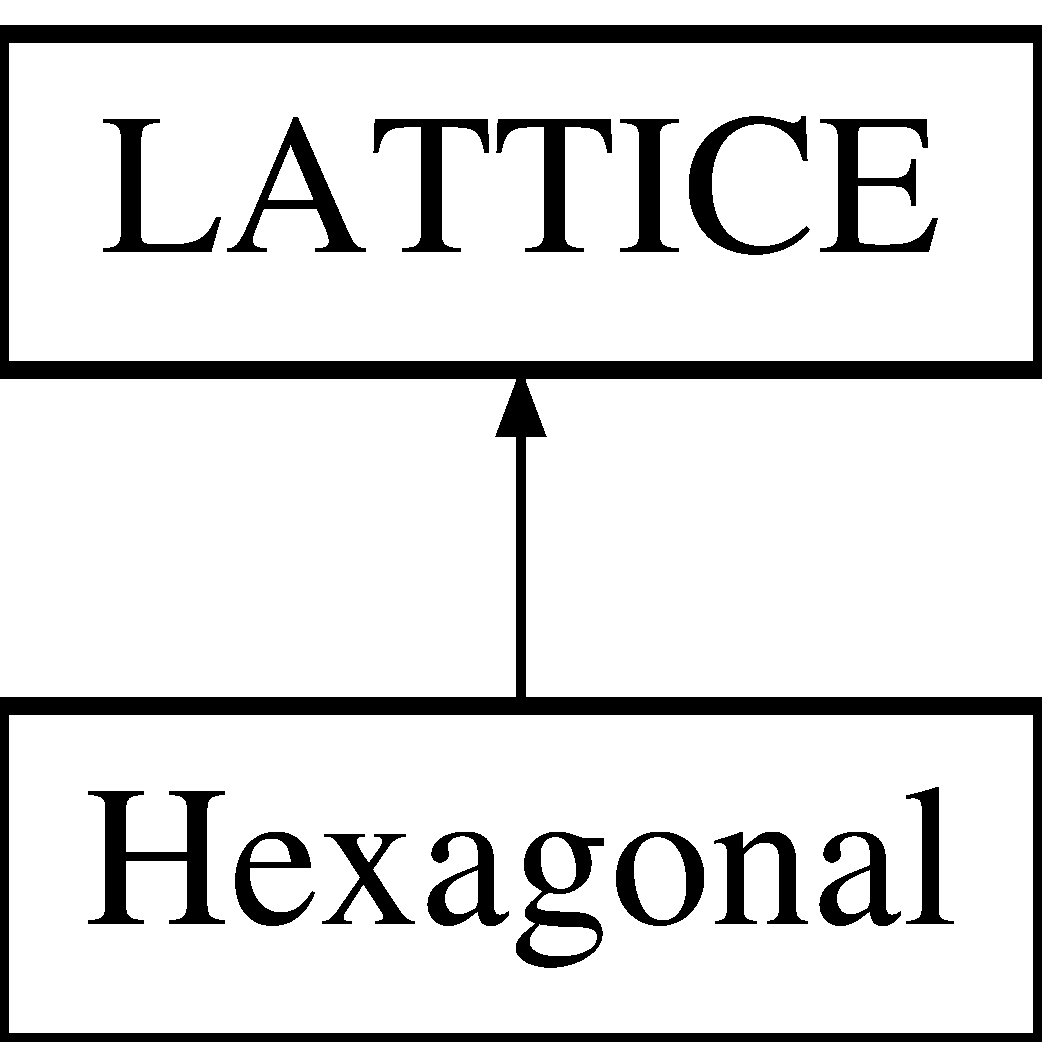
\includegraphics[height=2.000000cm]{class_hexagonal}
\end{center}
\end{figure}
\subsection*{Public Member Functions}
\begin{DoxyCompactItemize}
\item 
\hyperlink{class_hexagonal_adc3a73cb01ce229bfec31bb3a284a75b}{Hexagonal} (double i\+\_\+alat, char $\ast$i\+\_\+element)
\begin{DoxyCompactList}\small\item\em Constructor for the \hyperlink{class_orthorhombic}{Orthorhombic} class when accessed from a gui session or when reading a parameters file. \end{DoxyCompactList}\item 
\hyperlink{class_hexagonal_a972f325f1676b0bd7021c7d61b43311c}{$\sim$\+Hexagonal} ()
\end{DoxyCompactItemize}
\subsection*{Private Member Functions}
\begin{DoxyCompactItemize}
\item 
void \hyperlink{class_hexagonal_ae3e49df1849db3e8d865b5590cdfe18a}{primitive} ()
\begin{DoxyCompactList}\small\item\em Defines lattice vectors, lattice parameters, and basis atoms for H\+C\+P. \end{DoxyCompactList}\item 
void \hyperlink{class_hexagonal_af839a9f7a90a1d29bf972b45447eb4e0}{B\+C\+C} ()
\begin{DoxyCompactList}\small\item\em Defines lattice vectors, lattice parameters, and basis atoms for Body Centered \hyperlink{class_cubic}{Cubic}. \end{DoxyCompactList}\item 
void \hyperlink{class_hexagonal_adb86bd086e5ee120214a2bf246f96c16}{F\+C\+C} ()
\begin{DoxyCompactList}\small\item\em Defines lattice vectors, lattice parameters, and basis atoms for Face Centered \hyperlink{class_cubic}{Cubic}. \end{DoxyCompactList}\end{DoxyCompactItemize}
\subsection*{Additional Inherited Members}


\subsection{Constructor \& Destructor Documentation}
\hypertarget{class_hexagonal_adc3a73cb01ce229bfec31bb3a284a75b}{}\index{Hexagonal@{Hexagonal}!Hexagonal@{Hexagonal}}
\index{Hexagonal@{Hexagonal}!Hexagonal@{Hexagonal}}
\subsubsection[{Hexagonal}]{\setlength{\rightskip}{0pt plus 5cm}Hexagonal\+::\+Hexagonal (
\begin{DoxyParamCaption}
\item[{double}]{i\+\_\+alat, }
\item[{char $\ast$}]{i\+\_\+element}
\end{DoxyParamCaption}
)}\label{class_hexagonal_adc3a73cb01ce229bfec31bb3a284a75b}


Constructor for the \hyperlink{class_orthorhombic}{Orthorhombic} class when accessed from a gui session or when reading a parameters file. 


\begin{DoxyParams}[1]{Parameters}
\mbox{\tt in}  & {\em i\+\_\+alat} & -\/ lattice parameter for {\ttfamily a}, in Å \\
\hline
\mbox{\tt in}  & {\em i\+\_\+element} & -\/ which element to assign to the crystal \\
\hline
\end{DoxyParams}
\hypertarget{class_hexagonal_a972f325f1676b0bd7021c7d61b43311c}{}\index{Hexagonal@{Hexagonal}!````~Hexagonal@{$\sim$\+Hexagonal}}
\index{````~Hexagonal@{$\sim$\+Hexagonal}!Hexagonal@{Hexagonal}}
\subsubsection[{$\sim$\+Hexagonal}]{\setlength{\rightskip}{0pt plus 5cm}Hexagonal\+::$\sim$\+Hexagonal (
\begin{DoxyParamCaption}
{}
\end{DoxyParamCaption}
)}\label{class_hexagonal_a972f325f1676b0bd7021c7d61b43311c}


\subsection{Member Function Documentation}
\hypertarget{class_hexagonal_af839a9f7a90a1d29bf972b45447eb4e0}{}\index{Hexagonal@{Hexagonal}!B\+C\+C@{B\+C\+C}}
\index{B\+C\+C@{B\+C\+C}!Hexagonal@{Hexagonal}}
\subsubsection[{B\+C\+C}]{\setlength{\rightskip}{0pt plus 5cm}void Hexagonal\+::\+B\+C\+C (
\begin{DoxyParamCaption}
{}
\end{DoxyParamCaption}
)\hspace{0.3cm}{\ttfamily [private]}}\label{class_hexagonal_af839a9f7a90a1d29bf972b45447eb4e0}


Defines lattice vectors, lattice parameters, and basis atoms for Body Centered \hyperlink{class_cubic}{Cubic}. 

\hypertarget{class_hexagonal_adb86bd086e5ee120214a2bf246f96c16}{}\index{Hexagonal@{Hexagonal}!F\+C\+C@{F\+C\+C}}
\index{F\+C\+C@{F\+C\+C}!Hexagonal@{Hexagonal}}
\subsubsection[{F\+C\+C}]{\setlength{\rightskip}{0pt plus 5cm}void Hexagonal\+::\+F\+C\+C (
\begin{DoxyParamCaption}
{}
\end{DoxyParamCaption}
)\hspace{0.3cm}{\ttfamily [private]}}\label{class_hexagonal_adb86bd086e5ee120214a2bf246f96c16}


Defines lattice vectors, lattice parameters, and basis atoms for Face Centered \hyperlink{class_cubic}{Cubic}. 

\hypertarget{class_hexagonal_ae3e49df1849db3e8d865b5590cdfe18a}{}\index{Hexagonal@{Hexagonal}!primitive@{primitive}}
\index{primitive@{primitive}!Hexagonal@{Hexagonal}}
\subsubsection[{primitive}]{\setlength{\rightskip}{0pt plus 5cm}void Hexagonal\+::primitive (
\begin{DoxyParamCaption}
{}
\end{DoxyParamCaption}
)\hspace{0.3cm}{\ttfamily [private]}}\label{class_hexagonal_ae3e49df1849db3e8d865b5590cdfe18a}


Defines lattice vectors, lattice parameters, and basis atoms for H\+C\+P. 



The documentation for this class was generated from the following file\+:\begin{DoxyCompactItemize}
\item 
src/structures/\hyperlink{hexagonal_8h}{hexagonal.\+h}\end{DoxyCompactItemize}

\hypertarget{class_i_n_t_e_r_f_a_c_e}{}\section{I\+N\+T\+E\+R\+F\+A\+C\+E Class Reference}
\label{class_i_n_t_e_r_f_a_c_e}\index{I\+N\+T\+E\+R\+F\+A\+C\+E@{I\+N\+T\+E\+R\+F\+A\+C\+E}}


\subsection{Detailed Description}
\subsection*{{\bfseries Purpose\+:} }

\begin{DoxyVerb}/*****************************************************************************\
/  Class which constructs all of the core routines needed to build a crystal. \
/  Specifically, the Gui class, LATTICE class, and the Write class are all    \
/  constructed when this class is constructed.  This class serves to access   \
/  the data from Gui and send it to the LATTICE and Write classes.            \
/*****************************************************************************\
\end{DoxyVerb}


\begin{DoxyAuthor}{Author}
Joseph M. Gonzalez
\end{DoxyAuthor}
\begin{DoxyVersion}{Version}
0.\+2
\end{DoxyVersion}
\begin{DoxyDate}{Date}
Sep 13, 2015 19\+:16\+:20
\end{DoxyDate}
{\bfseries Contact} ~\newline
 \href{mailto:jmgonza6@mail.usf.edu}{\tt jmgonza6@mail.\+usf.\+edu} \subsection*{Public Member Functions}
\begin{DoxyCompactItemize}
\item 
\hyperlink{class_i_n_t_e_r_f_a_c_e_a62b3960b528d5220fe0a52e87382cc6e}{I\+N\+T\+E\+R\+F\+A\+C\+E} (int nargs, char $\ast$$\ast$argv, const char $\ast$fptr)
\begin{DoxyCompactList}\small\item\em Constructor to start up all core level classes. \end{DoxyCompactList}\item 
\hyperlink{class_i_n_t_e_r_f_a_c_e_aad406ae7418ff69f2c3131c67db2c736}{$\sim$\+I\+N\+T\+E\+R\+F\+A\+C\+E} ()
\begin{DoxyCompactList}\small\item\em Destructor to free all memory allocated for the core classes. \end{DoxyCompactList}\item 
void \hyperlink{class_i_n_t_e_r_f_a_c_e_a17e7bd199040a2aaf2b1d7d138e53759}{show\+\_\+parameters} ()
\begin{DoxyCompactList}\small\item\em Display all the parameters entered by the user during the G\+U\+I session. \end{DoxyCompactList}\item 
void \hyperlink{class_i_n_t_e_r_f_a_c_e_a71c1db660fb6a11b08b9144c999cb0ed}{build} ()
\begin{DoxyCompactList}\small\item\em Store all the parameters and build the required crystal. ~\newline
This is where each of the specific Bravais lattices are instantiated as an ~\newline
object of the \hyperlink{class_l_a_t_t_i_c_e}{L\+A\+T\+T\+I\+C\+E} class. \end{DoxyCompactList}\item 
void \hyperlink{class_i_n_t_e_r_f_a_c_e_a5f9daf84cbf9f286eadf64734c7a73d4}{build\+\_\+from\+\_\+file} ()
\begin{DoxyCompactList}\small\item\em Store all the parameters and build the required crystal. ~\newline
This is where each of the specific Bravais lattices are instantiated as an ~\newline
object of the \hyperlink{class_l_a_t_t_i_c_e}{L\+A\+T\+T\+I\+C\+E} class. \end{DoxyCompactList}\item 
void \hyperlink{class_i_n_t_e_r_f_a_c_e_ae00f42c78b8ad7323745e9b0cea1971c}{write\+\_\+data} (int src)
\begin{DoxyCompactList}\small\item\em \hyperlink{class_write}{Write} the as built crystal to a regular file. ~\newline
This method accesses the requested file format and passes all the necessary data for that format. \end{DoxyCompactList}\item 
int \hyperlink{class_i_n_t_e_r_f_a_c_e_a5811f0eaaa397ae3b72453774e424b67}{insane} ()
\begin{DoxyCompactList}\small\item\em Simple sanity check to ensure all necessary parameters have been defined .~\newline
 If a required parameter was not set, then a detailed message on the missing parameter~\newline
 is printed to the terminal via {\bfseries {\ttfamily stderr}}. \end{DoxyCompactList}\end{DoxyCompactItemize}
\subsection*{Data Fields}
\begin{DoxyCompactItemize}
\item 
std\+::vector$<$ std\+::string $>$ \hyperlink{class_i_n_t_e_r_f_a_c_e_aa55e1e42a1d2309638398bb640fbf74f}{species}
\begin{DoxyCompactList}\small\item\em container to hold each element string defined by the user \end{DoxyCompactList}\item 
\hyperlink{class_gui}{Gui} $\ast$ \hyperlink{class_i_n_t_e_r_f_a_c_e_a194a3b0540d87580158795d6a15d916e}{gui}
\begin{DoxyCompactList}\small\item\em pointer to the gui class \end{DoxyCompactList}\item 
\hyperlink{class_l_a_t_t_i_c_e}{L\+A\+T\+T\+I\+C\+E} $\ast$ \hyperlink{class_i_n_t_e_r_f_a_c_e_a5e07ee2e9ab4f84a9a6ae25c023dc24b}{lattice}
\begin{DoxyCompactList}\small\item\em pointer to the lattice class, each Bravais crystal inherits from \hyperlink{class_l_a_t_t_i_c_e}{L\+A\+T\+T\+I\+C\+E} \end{DoxyCompactList}\item 
\hyperlink{class_write}{Write} $\ast$ \hyperlink{class_i_n_t_e_r_f_a_c_e_a6e215284876b2bb79090fd3a210a40b0}{write}
\begin{DoxyCompactList}\small\item\em pointer to the write class, used for writing specific formats \end{DoxyCompactList}\item 
\hyperlink{class_errors}{Errors} $\ast$ \hyperlink{class_i_n_t_e_r_f_a_c_e_aeff8d391b9df980974a10c25b7667b33}{errors}
\item 
\hyperlink{class_parser}{Parser} $\ast$ \hyperlink{class_i_n_t_e_r_f_a_c_e_a71e1361007b1049a1c0012e4e72a672b}{parser}
\item 
\hyperlink{class_reader}{Reader} $\ast$ \hyperlink{class_i_n_t_e_r_f_a_c_e_a0b2f7b62040ca212b71dc2dbc9f8729a}{reader}
\end{DoxyCompactItemize}
\subsection*{Private Member Functions}
\begin{DoxyCompactItemize}
\item 
void \hyperlink{class_i_n_t_e_r_f_a_c_e_a4ae48a495e45c6a6a60cd3807209c851}{menu} ()
\begin{DoxyCompactList}\small\item\em Guide the user through an interactive command line menu to define the crystal parameters. ~\newline
Marked deprecated as of v 0.\+3! \end{DoxyCompactList}\item 
void \hyperlink{class_i_n_t_e_r_f_a_c_e_a2e2b70933b201b9f06ef12fc0f126035}{banner} ()
\begin{DoxyCompactList}\small\item\em Display program info at the command line. \end{DoxyCompactList}\item 
void \hyperlink{class_i_n_t_e_r_f_a_c_e_ae27d0174983d1e7fee1291e53858dc55}{input} (char $\ast$fptr)
\begin{DoxyCompactList}\small\item\em Read the atomic configuration from a text file. \end{DoxyCompactList}\end{DoxyCompactItemize}
\subsection*{Private Attributes}
\begin{DoxyCompactItemize}
\item 
double \hyperlink{class_i_n_t_e_r_f_a_c_e_acf38fe97c1ca8565367564059b195ed3}{i\+\_\+alat}
\item 
double \hyperlink{class_i_n_t_e_r_f_a_c_e_a22d766838fbda33270ff5c2773b18022}{i\+\_\+cta}
\item 
int \hyperlink{class_i_n_t_e_r_f_a_c_e_a1019e8f33030b94977af9d53dd18b2a2}{lclass}
\item 
int \hyperlink{class_i_n_t_e_r_f_a_c_e_a963ff0d6c9ea718dee31b4ea605f95f8}{lstyle}
\item 
int \hyperlink{class_i_n_t_e_r_f_a_c_e_a24698e299c30a479e6652e8a3ff1d805}{i\+\_\+lorient}
\item 
int \hyperlink{class_i_n_t_e_r_f_a_c_e_aa15d8db18b46f162fab82aaec313e898}{i\+\_\+species}
\item 
std\+::string \hyperlink{class_i_n_t_e_r_f_a_c_e_a36bed6ae97a342c0ae8ead780b0dfdf3}{atom\+\_\+list}
\item 
char $\ast$ \hyperlink{class_i_n_t_e_r_f_a_c_e_a5f1cd73e5b1dd4eebe65065e99967237}{oformat}
\item 
char $\ast$ \hyperlink{class_i_n_t_e_r_f_a_c_e_ae5e5c026e286c25b4baad2267cb2809c}{format}
\item 
char $\ast$ \hyperlink{class_i_n_t_e_r_f_a_c_e_a37fe82e9eb07354aa0396d0b35fae8d2}{fname}
\item 
char $\ast$ \hyperlink{class_i_n_t_e_r_f_a_c_e_afb94f9450b89e70f8b2396ec80f339da}{stylename}
\end{DoxyCompactItemize}


\subsection{Constructor \& Destructor Documentation}
\hypertarget{class_i_n_t_e_r_f_a_c_e_a62b3960b528d5220fe0a52e87382cc6e}{}\index{I\+N\+T\+E\+R\+F\+A\+C\+E@{I\+N\+T\+E\+R\+F\+A\+C\+E}!I\+N\+T\+E\+R\+F\+A\+C\+E@{I\+N\+T\+E\+R\+F\+A\+C\+E}}
\index{I\+N\+T\+E\+R\+F\+A\+C\+E@{I\+N\+T\+E\+R\+F\+A\+C\+E}!I\+N\+T\+E\+R\+F\+A\+C\+E@{I\+N\+T\+E\+R\+F\+A\+C\+E}}
\subsubsection[{I\+N\+T\+E\+R\+F\+A\+C\+E}]{\setlength{\rightskip}{0pt plus 5cm}I\+N\+T\+E\+R\+F\+A\+C\+E\+::\+I\+N\+T\+E\+R\+F\+A\+C\+E (
\begin{DoxyParamCaption}
\item[{int}]{nargs, }
\item[{char $\ast$$\ast$}]{argv, }
\item[{const char $\ast$}]{fptr}
\end{DoxyParamCaption}
)}\label{class_i_n_t_e_r_f_a_c_e_a62b3960b528d5220fe0a52e87382cc6e}


Constructor to start up all core level classes. 


\begin{DoxyParams}[1]{Parameters}
\mbox{\tt in}  & {\em nargs} & -\/ number of command line arguments \\
\hline
\mbox{\tt in}  & {\em argv} & -\/ char array containing all command line arguments \\
\hline
\mbox{\tt in}  & {\em fptr} & -\/ name of parameters file to read from \\
\hline
\end{DoxyParams}
\hypertarget{class_i_n_t_e_r_f_a_c_e_aad406ae7418ff69f2c3131c67db2c736}{}\index{I\+N\+T\+E\+R\+F\+A\+C\+E@{I\+N\+T\+E\+R\+F\+A\+C\+E}!````~I\+N\+T\+E\+R\+F\+A\+C\+E@{$\sim$\+I\+N\+T\+E\+R\+F\+A\+C\+E}}
\index{````~I\+N\+T\+E\+R\+F\+A\+C\+E@{$\sim$\+I\+N\+T\+E\+R\+F\+A\+C\+E}!I\+N\+T\+E\+R\+F\+A\+C\+E@{I\+N\+T\+E\+R\+F\+A\+C\+E}}
\subsubsection[{$\sim$\+I\+N\+T\+E\+R\+F\+A\+C\+E}]{\setlength{\rightskip}{0pt plus 5cm}I\+N\+T\+E\+R\+F\+A\+C\+E\+::$\sim$\+I\+N\+T\+E\+R\+F\+A\+C\+E (
\begin{DoxyParamCaption}
{}
\end{DoxyParamCaption}
)}\label{class_i_n_t_e_r_f_a_c_e_aad406ae7418ff69f2c3131c67db2c736}


Destructor to free all memory allocated for the core classes. 



\subsection{Member Function Documentation}
\hypertarget{class_i_n_t_e_r_f_a_c_e_a2e2b70933b201b9f06ef12fc0f126035}{}\index{I\+N\+T\+E\+R\+F\+A\+C\+E@{I\+N\+T\+E\+R\+F\+A\+C\+E}!banner@{banner}}
\index{banner@{banner}!I\+N\+T\+E\+R\+F\+A\+C\+E@{I\+N\+T\+E\+R\+F\+A\+C\+E}}
\subsubsection[{banner}]{\setlength{\rightskip}{0pt plus 5cm}void I\+N\+T\+E\+R\+F\+A\+C\+E\+::banner (
\begin{DoxyParamCaption}
{}
\end{DoxyParamCaption}
)\hspace{0.3cm}{\ttfamily [private]}}\label{class_i_n_t_e_r_f_a_c_e_a2e2b70933b201b9f06ef12fc0f126035}


Display program info at the command line. 

\hypertarget{class_i_n_t_e_r_f_a_c_e_a71c1db660fb6a11b08b9144c999cb0ed}{}\index{I\+N\+T\+E\+R\+F\+A\+C\+E@{I\+N\+T\+E\+R\+F\+A\+C\+E}!build@{build}}
\index{build@{build}!I\+N\+T\+E\+R\+F\+A\+C\+E@{I\+N\+T\+E\+R\+F\+A\+C\+E}}
\subsubsection[{build}]{\setlength{\rightskip}{0pt plus 5cm}void I\+N\+T\+E\+R\+F\+A\+C\+E\+::build (
\begin{DoxyParamCaption}
{}
\end{DoxyParamCaption}
)}\label{class_i_n_t_e_r_f_a_c_e_a71c1db660fb6a11b08b9144c999cb0ed}


Store all the parameters and build the required crystal. ~\newline
This is where each of the specific Bravais lattices are instantiated as an ~\newline
object of the \hyperlink{class_l_a_t_t_i_c_e}{L\+A\+T\+T\+I\+C\+E} class. 

\hypertarget{class_i_n_t_e_r_f_a_c_e_a5f9daf84cbf9f286eadf64734c7a73d4}{}\index{I\+N\+T\+E\+R\+F\+A\+C\+E@{I\+N\+T\+E\+R\+F\+A\+C\+E}!build\+\_\+from\+\_\+file@{build\+\_\+from\+\_\+file}}
\index{build\+\_\+from\+\_\+file@{build\+\_\+from\+\_\+file}!I\+N\+T\+E\+R\+F\+A\+C\+E@{I\+N\+T\+E\+R\+F\+A\+C\+E}}
\subsubsection[{build\+\_\+from\+\_\+file}]{\setlength{\rightskip}{0pt plus 5cm}void I\+N\+T\+E\+R\+F\+A\+C\+E\+::build\+\_\+from\+\_\+file (
\begin{DoxyParamCaption}
{}
\end{DoxyParamCaption}
)}\label{class_i_n_t_e_r_f_a_c_e_a5f9daf84cbf9f286eadf64734c7a73d4}


Store all the parameters and build the required crystal. ~\newline
This is where each of the specific Bravais lattices are instantiated as an ~\newline
object of the \hyperlink{class_l_a_t_t_i_c_e}{L\+A\+T\+T\+I\+C\+E} class. 

\hypertarget{class_i_n_t_e_r_f_a_c_e_ae27d0174983d1e7fee1291e53858dc55}{}\index{I\+N\+T\+E\+R\+F\+A\+C\+E@{I\+N\+T\+E\+R\+F\+A\+C\+E}!input@{input}}
\index{input@{input}!I\+N\+T\+E\+R\+F\+A\+C\+E@{I\+N\+T\+E\+R\+F\+A\+C\+E}}
\subsubsection[{input}]{\setlength{\rightskip}{0pt plus 5cm}void I\+N\+T\+E\+R\+F\+A\+C\+E\+::input (
\begin{DoxyParamCaption}
\item[{char $\ast$}]{fptr}
\end{DoxyParamCaption}
)\hspace{0.3cm}{\ttfamily [private]}}\label{class_i_n_t_e_r_f_a_c_e_ae27d0174983d1e7fee1291e53858dc55}


Read the atomic configuration from a text file. 


\begin{DoxyParams}[1]{Parameters}
\mbox{\tt in}  & {\em fptr} & -\/ Filename of the configuration file \\
\hline
\end{DoxyParams}
\hypertarget{class_i_n_t_e_r_f_a_c_e_a5811f0eaaa397ae3b72453774e424b67}{}\index{I\+N\+T\+E\+R\+F\+A\+C\+E@{I\+N\+T\+E\+R\+F\+A\+C\+E}!insane@{insane}}
\index{insane@{insane}!I\+N\+T\+E\+R\+F\+A\+C\+E@{I\+N\+T\+E\+R\+F\+A\+C\+E}}
\subsubsection[{insane}]{\setlength{\rightskip}{0pt plus 5cm}int I\+N\+T\+E\+R\+F\+A\+C\+E\+::insane (
\begin{DoxyParamCaption}
{}
\end{DoxyParamCaption}
)}\label{class_i_n_t_e_r_f_a_c_e_a5811f0eaaa397ae3b72453774e424b67}


Simple sanity check to ensure all necessary parameters have been defined .~\newline
 If a required parameter was not set, then a detailed message on the missing parameter~\newline
 is printed to the terminal via {\bfseries {\ttfamily stderr}}. 

\begin{DoxyReturn}{Returns}
{\ttfamily 0} if successful, {\ttfamily 1} otherwise 
\end{DoxyReturn}
\hypertarget{class_i_n_t_e_r_f_a_c_e_a4ae48a495e45c6a6a60cd3807209c851}{}\index{I\+N\+T\+E\+R\+F\+A\+C\+E@{I\+N\+T\+E\+R\+F\+A\+C\+E}!menu@{menu}}
\index{menu@{menu}!I\+N\+T\+E\+R\+F\+A\+C\+E@{I\+N\+T\+E\+R\+F\+A\+C\+E}}
\subsubsection[{menu}]{\setlength{\rightskip}{0pt plus 5cm}void I\+N\+T\+E\+R\+F\+A\+C\+E\+::menu (
\begin{DoxyParamCaption}
{}
\end{DoxyParamCaption}
)\hspace{0.3cm}{\ttfamily [private]}}\label{class_i_n_t_e_r_f_a_c_e_a4ae48a495e45c6a6a60cd3807209c851}


Guide the user through an interactive command line menu to define the crystal parameters. ~\newline
Marked deprecated as of v 0.\+3! 

\hypertarget{class_i_n_t_e_r_f_a_c_e_a17e7bd199040a2aaf2b1d7d138e53759}{}\index{I\+N\+T\+E\+R\+F\+A\+C\+E@{I\+N\+T\+E\+R\+F\+A\+C\+E}!show\+\_\+parameters@{show\+\_\+parameters}}
\index{show\+\_\+parameters@{show\+\_\+parameters}!I\+N\+T\+E\+R\+F\+A\+C\+E@{I\+N\+T\+E\+R\+F\+A\+C\+E}}
\subsubsection[{show\+\_\+parameters}]{\setlength{\rightskip}{0pt plus 5cm}void I\+N\+T\+E\+R\+F\+A\+C\+E\+::show\+\_\+parameters (
\begin{DoxyParamCaption}
{}
\end{DoxyParamCaption}
)}\label{class_i_n_t_e_r_f_a_c_e_a17e7bd199040a2aaf2b1d7d138e53759}


Display all the parameters entered by the user during the G\+U\+I session. 

\hypertarget{class_i_n_t_e_r_f_a_c_e_ae00f42c78b8ad7323745e9b0cea1971c}{}\index{I\+N\+T\+E\+R\+F\+A\+C\+E@{I\+N\+T\+E\+R\+F\+A\+C\+E}!write\+\_\+data@{write\+\_\+data}}
\index{write\+\_\+data@{write\+\_\+data}!I\+N\+T\+E\+R\+F\+A\+C\+E@{I\+N\+T\+E\+R\+F\+A\+C\+E}}
\subsubsection[{write\+\_\+data}]{\setlength{\rightskip}{0pt plus 5cm}void I\+N\+T\+E\+R\+F\+A\+C\+E\+::write\+\_\+data (
\begin{DoxyParamCaption}
\item[{int}]{src}
\end{DoxyParamCaption}
)}\label{class_i_n_t_e_r_f_a_c_e_ae00f42c78b8ad7323745e9b0cea1971c}


\hyperlink{class_write}{Write} the as built crystal to a regular file. ~\newline
This method accesses the requested file format and passes all the necessary data for that format. 



\subsection{Field Documentation}
\hypertarget{class_i_n_t_e_r_f_a_c_e_a36bed6ae97a342c0ae8ead780b0dfdf3}{}\index{I\+N\+T\+E\+R\+F\+A\+C\+E@{I\+N\+T\+E\+R\+F\+A\+C\+E}!atom\+\_\+list@{atom\+\_\+list}}
\index{atom\+\_\+list@{atom\+\_\+list}!I\+N\+T\+E\+R\+F\+A\+C\+E@{I\+N\+T\+E\+R\+F\+A\+C\+E}}
\subsubsection[{atom\+\_\+list}]{\setlength{\rightskip}{0pt plus 5cm}std\+::string I\+N\+T\+E\+R\+F\+A\+C\+E\+::atom\+\_\+list\hspace{0.3cm}{\ttfamily [private]}}\label{class_i_n_t_e_r_f_a_c_e_a36bed6ae97a342c0ae8ead780b0dfdf3}
\hypertarget{class_i_n_t_e_r_f_a_c_e_aeff8d391b9df980974a10c25b7667b33}{}\index{I\+N\+T\+E\+R\+F\+A\+C\+E@{I\+N\+T\+E\+R\+F\+A\+C\+E}!errors@{errors}}
\index{errors@{errors}!I\+N\+T\+E\+R\+F\+A\+C\+E@{I\+N\+T\+E\+R\+F\+A\+C\+E}}
\subsubsection[{errors}]{\setlength{\rightskip}{0pt plus 5cm}{\bf Errors}$\ast$ I\+N\+T\+E\+R\+F\+A\+C\+E\+::errors}\label{class_i_n_t_e_r_f_a_c_e_aeff8d391b9df980974a10c25b7667b33}
\hypertarget{class_i_n_t_e_r_f_a_c_e_a37fe82e9eb07354aa0396d0b35fae8d2}{}\index{I\+N\+T\+E\+R\+F\+A\+C\+E@{I\+N\+T\+E\+R\+F\+A\+C\+E}!fname@{fname}}
\index{fname@{fname}!I\+N\+T\+E\+R\+F\+A\+C\+E@{I\+N\+T\+E\+R\+F\+A\+C\+E}}
\subsubsection[{fname}]{\setlength{\rightskip}{0pt plus 5cm}char$\ast$ I\+N\+T\+E\+R\+F\+A\+C\+E\+::fname\hspace{0.3cm}{\ttfamily [private]}}\label{class_i_n_t_e_r_f_a_c_e_a37fe82e9eb07354aa0396d0b35fae8d2}
\hypertarget{class_i_n_t_e_r_f_a_c_e_ae5e5c026e286c25b4baad2267cb2809c}{}\index{I\+N\+T\+E\+R\+F\+A\+C\+E@{I\+N\+T\+E\+R\+F\+A\+C\+E}!format@{format}}
\index{format@{format}!I\+N\+T\+E\+R\+F\+A\+C\+E@{I\+N\+T\+E\+R\+F\+A\+C\+E}}
\subsubsection[{format}]{\setlength{\rightskip}{0pt plus 5cm}char$\ast$ I\+N\+T\+E\+R\+F\+A\+C\+E\+::format\hspace{0.3cm}{\ttfamily [private]}}\label{class_i_n_t_e_r_f_a_c_e_ae5e5c026e286c25b4baad2267cb2809c}
\hypertarget{class_i_n_t_e_r_f_a_c_e_a194a3b0540d87580158795d6a15d916e}{}\index{I\+N\+T\+E\+R\+F\+A\+C\+E@{I\+N\+T\+E\+R\+F\+A\+C\+E}!gui@{gui}}
\index{gui@{gui}!I\+N\+T\+E\+R\+F\+A\+C\+E@{I\+N\+T\+E\+R\+F\+A\+C\+E}}
\subsubsection[{gui}]{\setlength{\rightskip}{0pt plus 5cm}{\bf Gui}$\ast$ I\+N\+T\+E\+R\+F\+A\+C\+E\+::gui}\label{class_i_n_t_e_r_f_a_c_e_a194a3b0540d87580158795d6a15d916e}


pointer to the gui class 

\hypertarget{class_i_n_t_e_r_f_a_c_e_acf38fe97c1ca8565367564059b195ed3}{}\index{I\+N\+T\+E\+R\+F\+A\+C\+E@{I\+N\+T\+E\+R\+F\+A\+C\+E}!i\+\_\+alat@{i\+\_\+alat}}
\index{i\+\_\+alat@{i\+\_\+alat}!I\+N\+T\+E\+R\+F\+A\+C\+E@{I\+N\+T\+E\+R\+F\+A\+C\+E}}
\subsubsection[{i\+\_\+alat}]{\setlength{\rightskip}{0pt plus 5cm}double I\+N\+T\+E\+R\+F\+A\+C\+E\+::i\+\_\+alat\hspace{0.3cm}{\ttfamily [private]}}\label{class_i_n_t_e_r_f_a_c_e_acf38fe97c1ca8565367564059b195ed3}
\hypertarget{class_i_n_t_e_r_f_a_c_e_a22d766838fbda33270ff5c2773b18022}{}\index{I\+N\+T\+E\+R\+F\+A\+C\+E@{I\+N\+T\+E\+R\+F\+A\+C\+E}!i\+\_\+cta@{i\+\_\+cta}}
\index{i\+\_\+cta@{i\+\_\+cta}!I\+N\+T\+E\+R\+F\+A\+C\+E@{I\+N\+T\+E\+R\+F\+A\+C\+E}}
\subsubsection[{i\+\_\+cta}]{\setlength{\rightskip}{0pt plus 5cm}double I\+N\+T\+E\+R\+F\+A\+C\+E\+::i\+\_\+cta\hspace{0.3cm}{\ttfamily [private]}}\label{class_i_n_t_e_r_f_a_c_e_a22d766838fbda33270ff5c2773b18022}
\hypertarget{class_i_n_t_e_r_f_a_c_e_a24698e299c30a479e6652e8a3ff1d805}{}\index{I\+N\+T\+E\+R\+F\+A\+C\+E@{I\+N\+T\+E\+R\+F\+A\+C\+E}!i\+\_\+lorient@{i\+\_\+lorient}}
\index{i\+\_\+lorient@{i\+\_\+lorient}!I\+N\+T\+E\+R\+F\+A\+C\+E@{I\+N\+T\+E\+R\+F\+A\+C\+E}}
\subsubsection[{i\+\_\+lorient}]{\setlength{\rightskip}{0pt plus 5cm}int I\+N\+T\+E\+R\+F\+A\+C\+E\+::i\+\_\+lorient\hspace{0.3cm}{\ttfamily [private]}}\label{class_i_n_t_e_r_f_a_c_e_a24698e299c30a479e6652e8a3ff1d805}
\hypertarget{class_i_n_t_e_r_f_a_c_e_aa15d8db18b46f162fab82aaec313e898}{}\index{I\+N\+T\+E\+R\+F\+A\+C\+E@{I\+N\+T\+E\+R\+F\+A\+C\+E}!i\+\_\+species@{i\+\_\+species}}
\index{i\+\_\+species@{i\+\_\+species}!I\+N\+T\+E\+R\+F\+A\+C\+E@{I\+N\+T\+E\+R\+F\+A\+C\+E}}
\subsubsection[{i\+\_\+species}]{\setlength{\rightskip}{0pt plus 5cm}int I\+N\+T\+E\+R\+F\+A\+C\+E\+::i\+\_\+species\hspace{0.3cm}{\ttfamily [private]}}\label{class_i_n_t_e_r_f_a_c_e_aa15d8db18b46f162fab82aaec313e898}
\hypertarget{class_i_n_t_e_r_f_a_c_e_a5e07ee2e9ab4f84a9a6ae25c023dc24b}{}\index{I\+N\+T\+E\+R\+F\+A\+C\+E@{I\+N\+T\+E\+R\+F\+A\+C\+E}!lattice@{lattice}}
\index{lattice@{lattice}!I\+N\+T\+E\+R\+F\+A\+C\+E@{I\+N\+T\+E\+R\+F\+A\+C\+E}}
\subsubsection[{lattice}]{\setlength{\rightskip}{0pt plus 5cm}{\bf L\+A\+T\+T\+I\+C\+E}$\ast$ I\+N\+T\+E\+R\+F\+A\+C\+E\+::lattice}\label{class_i_n_t_e_r_f_a_c_e_a5e07ee2e9ab4f84a9a6ae25c023dc24b}


pointer to the lattice class, each Bravais crystal inherits from \hyperlink{class_l_a_t_t_i_c_e}{L\+A\+T\+T\+I\+C\+E} 

\hypertarget{class_i_n_t_e_r_f_a_c_e_a1019e8f33030b94977af9d53dd18b2a2}{}\index{I\+N\+T\+E\+R\+F\+A\+C\+E@{I\+N\+T\+E\+R\+F\+A\+C\+E}!lclass@{lclass}}
\index{lclass@{lclass}!I\+N\+T\+E\+R\+F\+A\+C\+E@{I\+N\+T\+E\+R\+F\+A\+C\+E}}
\subsubsection[{lclass}]{\setlength{\rightskip}{0pt plus 5cm}int I\+N\+T\+E\+R\+F\+A\+C\+E\+::lclass\hspace{0.3cm}{\ttfamily [private]}}\label{class_i_n_t_e_r_f_a_c_e_a1019e8f33030b94977af9d53dd18b2a2}
\hypertarget{class_i_n_t_e_r_f_a_c_e_a963ff0d6c9ea718dee31b4ea605f95f8}{}\index{I\+N\+T\+E\+R\+F\+A\+C\+E@{I\+N\+T\+E\+R\+F\+A\+C\+E}!lstyle@{lstyle}}
\index{lstyle@{lstyle}!I\+N\+T\+E\+R\+F\+A\+C\+E@{I\+N\+T\+E\+R\+F\+A\+C\+E}}
\subsubsection[{lstyle}]{\setlength{\rightskip}{0pt plus 5cm}int I\+N\+T\+E\+R\+F\+A\+C\+E\+::lstyle\hspace{0.3cm}{\ttfamily [private]}}\label{class_i_n_t_e_r_f_a_c_e_a963ff0d6c9ea718dee31b4ea605f95f8}
\hypertarget{class_i_n_t_e_r_f_a_c_e_a5f1cd73e5b1dd4eebe65065e99967237}{}\index{I\+N\+T\+E\+R\+F\+A\+C\+E@{I\+N\+T\+E\+R\+F\+A\+C\+E}!oformat@{oformat}}
\index{oformat@{oformat}!I\+N\+T\+E\+R\+F\+A\+C\+E@{I\+N\+T\+E\+R\+F\+A\+C\+E}}
\subsubsection[{oformat}]{\setlength{\rightskip}{0pt plus 5cm}char$\ast$ I\+N\+T\+E\+R\+F\+A\+C\+E\+::oformat\hspace{0.3cm}{\ttfamily [private]}}\label{class_i_n_t_e_r_f_a_c_e_a5f1cd73e5b1dd4eebe65065e99967237}
\hypertarget{class_i_n_t_e_r_f_a_c_e_a71e1361007b1049a1c0012e4e72a672b}{}\index{I\+N\+T\+E\+R\+F\+A\+C\+E@{I\+N\+T\+E\+R\+F\+A\+C\+E}!parser@{parser}}
\index{parser@{parser}!I\+N\+T\+E\+R\+F\+A\+C\+E@{I\+N\+T\+E\+R\+F\+A\+C\+E}}
\subsubsection[{parser}]{\setlength{\rightskip}{0pt plus 5cm}{\bf Parser}$\ast$ I\+N\+T\+E\+R\+F\+A\+C\+E\+::parser}\label{class_i_n_t_e_r_f_a_c_e_a71e1361007b1049a1c0012e4e72a672b}
\hypertarget{class_i_n_t_e_r_f_a_c_e_a0b2f7b62040ca212b71dc2dbc9f8729a}{}\index{I\+N\+T\+E\+R\+F\+A\+C\+E@{I\+N\+T\+E\+R\+F\+A\+C\+E}!reader@{reader}}
\index{reader@{reader}!I\+N\+T\+E\+R\+F\+A\+C\+E@{I\+N\+T\+E\+R\+F\+A\+C\+E}}
\subsubsection[{reader}]{\setlength{\rightskip}{0pt plus 5cm}{\bf Reader}$\ast$ I\+N\+T\+E\+R\+F\+A\+C\+E\+::reader}\label{class_i_n_t_e_r_f_a_c_e_a0b2f7b62040ca212b71dc2dbc9f8729a}
\hypertarget{class_i_n_t_e_r_f_a_c_e_aa55e1e42a1d2309638398bb640fbf74f}{}\index{I\+N\+T\+E\+R\+F\+A\+C\+E@{I\+N\+T\+E\+R\+F\+A\+C\+E}!species@{species}}
\index{species@{species}!I\+N\+T\+E\+R\+F\+A\+C\+E@{I\+N\+T\+E\+R\+F\+A\+C\+E}}
\subsubsection[{species}]{\setlength{\rightskip}{0pt plus 5cm}std\+::vector$<$std\+::string$>$ I\+N\+T\+E\+R\+F\+A\+C\+E\+::species}\label{class_i_n_t_e_r_f_a_c_e_aa55e1e42a1d2309638398bb640fbf74f}


container to hold each element string defined by the user 

\hypertarget{class_i_n_t_e_r_f_a_c_e_afb94f9450b89e70f8b2396ec80f339da}{}\index{I\+N\+T\+E\+R\+F\+A\+C\+E@{I\+N\+T\+E\+R\+F\+A\+C\+E}!stylename@{stylename}}
\index{stylename@{stylename}!I\+N\+T\+E\+R\+F\+A\+C\+E@{I\+N\+T\+E\+R\+F\+A\+C\+E}}
\subsubsection[{stylename}]{\setlength{\rightskip}{0pt plus 5cm}char$\ast$ I\+N\+T\+E\+R\+F\+A\+C\+E\+::stylename\hspace{0.3cm}{\ttfamily [private]}}\label{class_i_n_t_e_r_f_a_c_e_afb94f9450b89e70f8b2396ec80f339da}
\hypertarget{class_i_n_t_e_r_f_a_c_e_a6e215284876b2bb79090fd3a210a40b0}{}\index{I\+N\+T\+E\+R\+F\+A\+C\+E@{I\+N\+T\+E\+R\+F\+A\+C\+E}!write@{write}}
\index{write@{write}!I\+N\+T\+E\+R\+F\+A\+C\+E@{I\+N\+T\+E\+R\+F\+A\+C\+E}}
\subsubsection[{write}]{\setlength{\rightskip}{0pt plus 5cm}{\bf Write}$\ast$ I\+N\+T\+E\+R\+F\+A\+C\+E\+::write}\label{class_i_n_t_e_r_f_a_c_e_a6e215284876b2bb79090fd3a210a40b0}


pointer to the write class, used for writing specific formats 



The documentation for this class was generated from the following file\+:\begin{DoxyCompactItemize}
\item 
src/main/\hyperlink{interface_8h}{interface.\+h}\end{DoxyCompactItemize}

\hypertarget{class_l_a_t_t_i_c_e}{}\section{L\+A\+T\+T\+I\+C\+E Class Reference}
\label{class_l_a_t_t_i_c_e}\index{L\+A\+T\+T\+I\+C\+E@{L\+A\+T\+T\+I\+C\+E}}


\subsection{Detailed Description}
\begin{quote}


{\bfseries Purpose\+:} 

\end{quote}
\begin{DoxyVerb}*
*  Base class for constructing an arbitrary crystal structure based 
*  on the fractional coordinates of the basis atoms, lattice vectors
*  and lattice parameters a,b,c.
*
* \end{DoxyVerb}
 \begin{quote}
\begin{DoxyAuthor}{Author}
Joseph M. Gonzalez
\end{DoxyAuthor}
\begin{DoxyVersion}{Version}
0.\+2
\end{DoxyVersion}
\begin{DoxyDate}{Date}
Sep 13, 2015 19\+:16\+:20
\end{DoxyDate}
{\bfseries Contact} ~\newline
 \href{mailto:jmgonza6@mail.usf.edu}{\tt jmgonza6@mail.\+usf.\+edu}\end{quote}
Inheritance diagram for L\+A\+T\+T\+I\+C\+E\+:\begin{figure}[H]
\begin{center}
\leavevmode
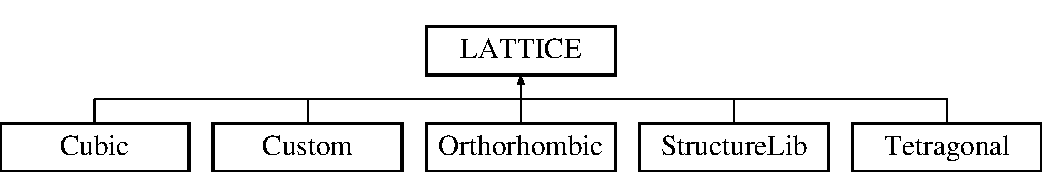
\includegraphics[height=2.000000cm]{class_l_a_t_t_i_c_e}
\end{center}
\end{figure}
\subsection*{Public Member Functions}
\begin{DoxyCompactItemize}
\item 
\hyperlink{structatom__t}{atom\+\_\+t} $\ast$ \hyperlink{class_l_a_t_t_i_c_e_a3a2222333e6da3cb42954bc1c66f9c44}{copy\+\_\+data} (\hyperlink{structatom__t}{atom\+\_\+t} $\ast$atoms\+I)
\item 
\hyperlink{class_l_a_t_t_i_c_e_aabfd2a1302dd09ab010cf26414175436}{L\+A\+T\+T\+I\+C\+E} ()
\item 
\hyperlink{class_l_a_t_t_i_c_e_a2e6f18c8b01ca4bbed6132603ade137e}{$\sim$\+L\+A\+T\+T\+I\+C\+E} ()
\item 
void \hyperlink{class_l_a_t_t_i_c_e_a9dd17973a1e8c445663553864f82bea6}{show\+\_\+info} ()
\begin{DoxyCompactList}\small\item\em Display all parameters set during the G\+U\+I session. \end{DoxyCompactList}\item 
int \hyperlink{class_l_a_t_t_i_c_e_aba8ae41405acc746ae6294dd0ad67f96}{convert\+\_\+coordinates} (int \hyperlink{class_l_a_t_t_i_c_e_a922caeabeb80ebdc3c899b64eaf527ac}{fractional})
\begin{DoxyCompactList}\small\item\em Convert the cartesian atomic coordinates to fractional before writing the data. \end{DoxyCompactList}\item 
void \hyperlink{class_l_a_t_t_i_c_e_a764395141f8545e8b2dc237371c177ad}{build\+\_\+crystal} ()
\begin{DoxyCompactList}\small\item\em Start the build process using the parameters set during the G\+U\+I session. \end{DoxyCompactList}\end{DoxyCompactItemize}
\subsection*{Data Fields}
\begin{DoxyCompactItemize}
\item 
\hyperlink{class_memory}{Memory} $\ast$ \hyperlink{class_l_a_t_t_i_c_e_a4e8795a8cbd0a4594657a071fe68b9c3}{memory}
\begin{DoxyCompactList}\small\item\em pointer to memory allocation handler \end{DoxyCompactList}\item 
\hyperlink{structatom__t}{atom\+\_\+t} $\ast$ \hyperlink{class_l_a_t_t_i_c_e_aeb9f05d5a05013f9e39771004ee7a351}{atoms}
\begin{DoxyCompactList}\small\item\em internal structure to hold atomic info \end{DoxyCompactList}\item 
\hyperlink{structatom__t}{atom\+\_\+t} $\ast$ \hyperlink{class_l_a_t_t_i_c_e_a529b0104c83d19577c69688fa247238c}{atoms\+Out}
\begin{DoxyCompactList}\small\item\em structure for output atomic info \end{DoxyCompactList}\item 
\hyperlink{structbasis__t}{basis\+\_\+t} $\ast$ \hyperlink{class_l_a_t_t_i_c_e_a6af830d3ced50888840f85a837a730e1}{basis}
\begin{DoxyCompactList}\small\item\em structure for basis atoms in single unit cell \end{DoxyCompactList}\item 
double \hyperlink{class_l_a_t_t_i_c_e_a0b631e7b0ab66a25bf15fbf49d684f07}{alat}
\begin{DoxyCompactList}\small\item\em a lattice constant \end{DoxyCompactList}\item 
double \hyperlink{class_l_a_t_t_i_c_e_ae125b693205deca9ed500e9ece8c4f2d}{blat}
\begin{DoxyCompactList}\small\item\em b lattice constant \end{DoxyCompactList}\item 
double \hyperlink{class_l_a_t_t_i_c_e_aae495a347749c2380c73ecb89b955f3d}{clat}
\begin{DoxyCompactList}\small\item\em c lattice constant \end{DoxyCompactList}\item 
double \hyperlink{class_l_a_t_t_i_c_e_af8ceb04d3e61325053e42df2c797064d}{alpha}
\begin{DoxyCompactList}\small\item\em angle between {\ttfamily b \& c} \end{DoxyCompactList}\item 
double \hyperlink{class_l_a_t_t_i_c_e_ad16b52e37b1f6f92598aec8940503bf3}{beta}
\begin{DoxyCompactList}\small\item\em angle between {\ttfamily a \& c} \end{DoxyCompactList}\item 
double \hyperlink{class_l_a_t_t_i_c_e_a5a4c56af589d9fa6639025ef72e8fac2}{gamma}
\begin{DoxyCompactList}\small\item\em angle between {\ttfamily a \& b} \end{DoxyCompactList}\item 
std\+::vector$<$ double $>$ \hyperlink{class_l_a_t_t_i_c_e_a9a56f2f8e797ae6a496527f1ba937769}{a1}
\begin{DoxyCompactList}\small\item\em a lattice vector, along \mbox{[}100\mbox{]} \end{DoxyCompactList}\item 
std\+::vector$<$ double $>$ \hyperlink{class_l_a_t_t_i_c_e_a7f6dbfc6795b67a0d92b156789bb8977}{a2}
\begin{DoxyCompactList}\small\item\em b lattice vector, somewhere along \mbox{[}110\mbox{]} \end{DoxyCompactList}\item 
std\+::vector$<$ double $>$ \hyperlink{class_l_a_t_t_i_c_e_a5f5355169d092e243480783bde501ccd}{a3}
\begin{DoxyCompactList}\small\item\em c lattice vector, somewhere along \mbox{[}111\mbox{]} \end{DoxyCompactList}\item 
int $\ast$ \hyperlink{class_l_a_t_t_i_c_e_a8eb1ea5b25b8678b136c5e663d4aeb0e}{atom\+\_\+type}
\begin{DoxyCompactList}\small\item\em pointer to hold all unique types \end{DoxyCompactList}\item 
int \hyperlink{class_l_a_t_t_i_c_e_a9efda355b82d0fcbc013b1fdf17bb758}{natom}
\begin{DoxyCompactList}\small\item\em total atoms created \end{DoxyCompactList}\item 
int \hyperlink{class_l_a_t_t_i_c_e_acf531dce17fd666a58e9007615bc51eb}{apcell}
\begin{DoxyCompactList}\small\item\em number of atoms in a single unit cell \end{DoxyCompactList}\item 
int \hyperlink{class_l_a_t_t_i_c_e_a552cdb99c1b6cc2bd8bdd723e9f141ab}{ntype}
\begin{DoxyCompactList}\small\item\em number of atoms and atomic types in a unit cell \end{DoxyCompactList}\item 
int \hyperlink{class_l_a_t_t_i_c_e_a64884f89e993db7a215153bf5f56987b}{nx}
\begin{DoxyCompactList}\small\item\em number of unit along a1 \end{DoxyCompactList}\item 
int \hyperlink{class_l_a_t_t_i_c_e_aa202fceba51fcd040afafd1a02e2860e}{ny}
\begin{DoxyCompactList}\small\item\em number of unit along a2 \end{DoxyCompactList}\item 
int \hyperlink{class_l_a_t_t_i_c_e_ad32ea9361884a2bbcb81714ebe1bc15c}{nz}
\begin{DoxyCompactList}\small\item\em number of unit along a3 \end{DoxyCompactList}\item 
int \hyperlink{class_l_a_t_t_i_c_e_a922caeabeb80ebdc3c899b64eaf527ac}{fractional}
\begin{DoxyCompactList}\small\item\em {\ttfamily 1} if the output coordinates are fractional, {\ttfamily 0} otherwise \end{DoxyCompactList}\item 
char $\ast$ \hyperlink{class_l_a_t_t_i_c_e_ac1c63af3a896cf4d443347cd202698f7}{fformat}
\begin{DoxyCompactList}\small\item\em output file format, lammps, vasp, dmol \end{DoxyCompactList}\item 
char $\ast$ \hyperlink{class_l_a_t_t_i_c_e_ad986fd67c523ad7201ba9deaefcf6543}{name}
\begin{DoxyCompactList}\small\item\em name of the Bravais lattice, \hyperlink{class_cubic}{Cubic}, \hyperlink{class_tetragonal}{Tetragonal}, Graphene ... \end{DoxyCompactList}\item 
char $\ast$ \hyperlink{class_l_a_t_t_i_c_e_a07635742a674cf3203f8e2c5c48118f8}{lstyle}
\begin{DoxyCompactList}\small\item\em style of the Bravais lattice \end{DoxyCompactList}\item 
std\+::vector$<$ std\+::string $>$ \hyperlink{class_l_a_t_t_i_c_e_a3737ca172950824ad0ab699802f26417}{species}
\begin{DoxyCompactList}\small\item\em vector containing unique element symbols \end{DoxyCompactList}\item 
std\+::vector$<$ int $>$ \hyperlink{class_l_a_t_t_i_c_e_a63bb555fee4e3cc086f0826437aa5af8}{elem\+Count}
\item 
std\+::vector$<$ int $>$ \hyperlink{class_l_a_t_t_i_c_e_aff3f0cdf099776c7c3dc5257e38aa52f}{type\+Count}
\begin{DoxyCompactList}\small\item\em keep track of how many of each type, {\ttfamily type\+Count\mbox{[}0\mbox{]} -\/$>$ type 1 ...} \end{DoxyCompactList}\end{DoxyCompactItemize}
\subsection*{Private Member Functions}
\begin{DoxyCompactItemize}
\item 
\hyperlink{structatom__t}{atom\+\_\+t} $\ast$ \hyperlink{class_l_a_t_t_i_c_e_ad3ac8f3bbd9f44abe61b8b7ceb62c563}{cart2fract} (std\+::vector$<$ double $>$ \hyperlink{class_l_a_t_t_i_c_e_a9a56f2f8e797ae6a496527f1ba937769}{a1}, std\+::vector$<$ double $>$ \hyperlink{class_l_a_t_t_i_c_e_a7f6dbfc6795b67a0d92b156789bb8977}{a2}, std\+::vector$<$ double $>$ \hyperlink{class_l_a_t_t_i_c_e_a5f5355169d092e243480783bde501ccd}{a3}, \hyperlink{structatom__t}{atom\+\_\+t} $\ast$atoms\+I)
\begin{DoxyCompactList}\small\item\em Convert the cartesian coordinates to fractional before writing the data. \end{DoxyCompactList}\item 
void \hyperlink{class_l_a_t_t_i_c_e_ad5df57f16ebd026cfccf59eaa5e9089f}{nn\+\_\+search} ()
\end{DoxyCompactItemize}


\subsection{Constructor \& Destructor Documentation}
\hypertarget{class_l_a_t_t_i_c_e_aabfd2a1302dd09ab010cf26414175436}{}\index{L\+A\+T\+T\+I\+C\+E@{L\+A\+T\+T\+I\+C\+E}!L\+A\+T\+T\+I\+C\+E@{L\+A\+T\+T\+I\+C\+E}}
\index{L\+A\+T\+T\+I\+C\+E@{L\+A\+T\+T\+I\+C\+E}!L\+A\+T\+T\+I\+C\+E@{L\+A\+T\+T\+I\+C\+E}}
\subsubsection[{L\+A\+T\+T\+I\+C\+E}]{\setlength{\rightskip}{0pt plus 5cm}L\+A\+T\+T\+I\+C\+E\+::\+L\+A\+T\+T\+I\+C\+E (
\begin{DoxyParamCaption}
{}
\end{DoxyParamCaption}
)}\label{class_l_a_t_t_i_c_e_aabfd2a1302dd09ab010cf26414175436}
\hypertarget{class_l_a_t_t_i_c_e_a2e6f18c8b01ca4bbed6132603ade137e}{}\index{L\+A\+T\+T\+I\+C\+E@{L\+A\+T\+T\+I\+C\+E}!````~L\+A\+T\+T\+I\+C\+E@{$\sim$\+L\+A\+T\+T\+I\+C\+E}}
\index{````~L\+A\+T\+T\+I\+C\+E@{$\sim$\+L\+A\+T\+T\+I\+C\+E}!L\+A\+T\+T\+I\+C\+E@{L\+A\+T\+T\+I\+C\+E}}
\subsubsection[{$\sim$\+L\+A\+T\+T\+I\+C\+E}]{\setlength{\rightskip}{0pt plus 5cm}L\+A\+T\+T\+I\+C\+E\+::$\sim$\+L\+A\+T\+T\+I\+C\+E (
\begin{DoxyParamCaption}
{}
\end{DoxyParamCaption}
)}\label{class_l_a_t_t_i_c_e_a2e6f18c8b01ca4bbed6132603ade137e}


\subsection{Member Function Documentation}
\hypertarget{class_l_a_t_t_i_c_e_a764395141f8545e8b2dc237371c177ad}{}\index{L\+A\+T\+T\+I\+C\+E@{L\+A\+T\+T\+I\+C\+E}!build\+\_\+crystal@{build\+\_\+crystal}}
\index{build\+\_\+crystal@{build\+\_\+crystal}!L\+A\+T\+T\+I\+C\+E@{L\+A\+T\+T\+I\+C\+E}}
\subsubsection[{build\+\_\+crystal}]{\setlength{\rightskip}{0pt plus 5cm}void L\+A\+T\+T\+I\+C\+E\+::build\+\_\+crystal (
\begin{DoxyParamCaption}
{}
\end{DoxyParamCaption}
)}\label{class_l_a_t_t_i_c_e_a764395141f8545e8b2dc237371c177ad}


Start the build process using the parameters set during the G\+U\+I session. 

\hypertarget{class_l_a_t_t_i_c_e_ad3ac8f3bbd9f44abe61b8b7ceb62c563}{}\index{L\+A\+T\+T\+I\+C\+E@{L\+A\+T\+T\+I\+C\+E}!cart2fract@{cart2fract}}
\index{cart2fract@{cart2fract}!L\+A\+T\+T\+I\+C\+E@{L\+A\+T\+T\+I\+C\+E}}
\subsubsection[{cart2fract}]{\setlength{\rightskip}{0pt plus 5cm}{\bf atom\+\_\+t}$\ast$ L\+A\+T\+T\+I\+C\+E\+::cart2fract (
\begin{DoxyParamCaption}
\item[{std\+::vector$<$ double $>$}]{a1, }
\item[{std\+::vector$<$ double $>$}]{a2, }
\item[{std\+::vector$<$ double $>$}]{a3, }
\item[{{\bf atom\+\_\+t} $\ast$}]{atoms\+I}
\end{DoxyParamCaption}
)\hspace{0.3cm}{\ttfamily [private]}}\label{class_l_a_t_t_i_c_e_ad3ac8f3bbd9f44abe61b8b7ceb62c563}


Convert the cartesian coordinates to fractional before writing the data. 


\begin{DoxyParams}[1]{Parameters}
\mbox{\tt in}  & {\em a1} & -\/ major lattice vector, in cartesian coordinates \\
\hline
\mbox{\tt in}  & {\em a2} & -\/ lattice vector, in {\ttfamily xy plane}, in cartesian coordinates \\
\hline
\mbox{\tt in}  & {\em a3} & -\/ lattice vector, in {\ttfamily xyz plane}, in cartesian coordinates \\
\hline
\mbox{\tt in}  & {\em atoms\+I} & -\/ 1\+D struct containing the atomic coordinates in \\
\hline
\end{DoxyParams}
\hypertarget{class_l_a_t_t_i_c_e_aba8ae41405acc746ae6294dd0ad67f96}{}\index{L\+A\+T\+T\+I\+C\+E@{L\+A\+T\+T\+I\+C\+E}!convert\+\_\+coordinates@{convert\+\_\+coordinates}}
\index{convert\+\_\+coordinates@{convert\+\_\+coordinates}!L\+A\+T\+T\+I\+C\+E@{L\+A\+T\+T\+I\+C\+E}}
\subsubsection[{convert\+\_\+coordinates}]{\setlength{\rightskip}{0pt plus 5cm}int L\+A\+T\+T\+I\+C\+E\+::convert\+\_\+coordinates (
\begin{DoxyParamCaption}
\item[{int}]{fractional}
\end{DoxyParamCaption}
)}\label{class_l_a_t_t_i_c_e_aba8ae41405acc746ae6294dd0ad67f96}


Convert the cartesian atomic coordinates to fractional before writing the data. 


\begin{DoxyParams}[1]{Parameters}
\mbox{\tt in}  & {\em fractional} & -\/ {\itshape 1} if fractional {\itshape 0} otherwise \\
\hline
\end{DoxyParams}
\begin{DoxyReturn}{Returns}
1 if successful 
\end{DoxyReturn}
\hypertarget{class_l_a_t_t_i_c_e_a3a2222333e6da3cb42954bc1c66f9c44}{}\index{L\+A\+T\+T\+I\+C\+E@{L\+A\+T\+T\+I\+C\+E}!copy\+\_\+data@{copy\+\_\+data}}
\index{copy\+\_\+data@{copy\+\_\+data}!L\+A\+T\+T\+I\+C\+E@{L\+A\+T\+T\+I\+C\+E}}
\subsubsection[{copy\+\_\+data}]{\setlength{\rightskip}{0pt plus 5cm}{\bf atom\+\_\+t}$\ast$ L\+A\+T\+T\+I\+C\+E\+::copy\+\_\+data (
\begin{DoxyParamCaption}
\item[{{\bf atom\+\_\+t} $\ast$}]{atoms\+I}
\end{DoxyParamCaption}
)}\label{class_l_a_t_t_i_c_e_a3a2222333e6da3cb42954bc1c66f9c44}
\hypertarget{class_l_a_t_t_i_c_e_ad5df57f16ebd026cfccf59eaa5e9089f}{}\index{L\+A\+T\+T\+I\+C\+E@{L\+A\+T\+T\+I\+C\+E}!nn\+\_\+search@{nn\+\_\+search}}
\index{nn\+\_\+search@{nn\+\_\+search}!L\+A\+T\+T\+I\+C\+E@{L\+A\+T\+T\+I\+C\+E}}
\subsubsection[{nn\+\_\+search}]{\setlength{\rightskip}{0pt plus 5cm}void L\+A\+T\+T\+I\+C\+E\+::nn\+\_\+search (
\begin{DoxyParamCaption}
{}
\end{DoxyParamCaption}
)\hspace{0.3cm}{\ttfamily [private]}}\label{class_l_a_t_t_i_c_e_ad5df57f16ebd026cfccf59eaa5e9089f}
\hypertarget{class_l_a_t_t_i_c_e_a9dd17973a1e8c445663553864f82bea6}{}\index{L\+A\+T\+T\+I\+C\+E@{L\+A\+T\+T\+I\+C\+E}!show\+\_\+info@{show\+\_\+info}}
\index{show\+\_\+info@{show\+\_\+info}!L\+A\+T\+T\+I\+C\+E@{L\+A\+T\+T\+I\+C\+E}}
\subsubsection[{show\+\_\+info}]{\setlength{\rightskip}{0pt plus 5cm}void L\+A\+T\+T\+I\+C\+E\+::show\+\_\+info (
\begin{DoxyParamCaption}
{}
\end{DoxyParamCaption}
)}\label{class_l_a_t_t_i_c_e_a9dd17973a1e8c445663553864f82bea6}


Display all parameters set during the G\+U\+I session. 



\subsection{Field Documentation}
\hypertarget{class_l_a_t_t_i_c_e_a9a56f2f8e797ae6a496527f1ba937769}{}\index{L\+A\+T\+T\+I\+C\+E@{L\+A\+T\+T\+I\+C\+E}!a1@{a1}}
\index{a1@{a1}!L\+A\+T\+T\+I\+C\+E@{L\+A\+T\+T\+I\+C\+E}}
\subsubsection[{a1}]{\setlength{\rightskip}{0pt plus 5cm}std\+::vector$<$double$>$ L\+A\+T\+T\+I\+C\+E\+::a1}\label{class_l_a_t_t_i_c_e_a9a56f2f8e797ae6a496527f1ba937769}


a lattice vector, along \mbox{[}100\mbox{]} 

\hypertarget{class_l_a_t_t_i_c_e_a7f6dbfc6795b67a0d92b156789bb8977}{}\index{L\+A\+T\+T\+I\+C\+E@{L\+A\+T\+T\+I\+C\+E}!a2@{a2}}
\index{a2@{a2}!L\+A\+T\+T\+I\+C\+E@{L\+A\+T\+T\+I\+C\+E}}
\subsubsection[{a2}]{\setlength{\rightskip}{0pt plus 5cm}std\+::vector$<$double$>$ L\+A\+T\+T\+I\+C\+E\+::a2}\label{class_l_a_t_t_i_c_e_a7f6dbfc6795b67a0d92b156789bb8977}


b lattice vector, somewhere along \mbox{[}110\mbox{]} 

\hypertarget{class_l_a_t_t_i_c_e_a5f5355169d092e243480783bde501ccd}{}\index{L\+A\+T\+T\+I\+C\+E@{L\+A\+T\+T\+I\+C\+E}!a3@{a3}}
\index{a3@{a3}!L\+A\+T\+T\+I\+C\+E@{L\+A\+T\+T\+I\+C\+E}}
\subsubsection[{a3}]{\setlength{\rightskip}{0pt plus 5cm}std\+::vector$<$double$>$ L\+A\+T\+T\+I\+C\+E\+::a3}\label{class_l_a_t_t_i_c_e_a5f5355169d092e243480783bde501ccd}


c lattice vector, somewhere along \mbox{[}111\mbox{]} 

\hypertarget{class_l_a_t_t_i_c_e_a0b631e7b0ab66a25bf15fbf49d684f07}{}\index{L\+A\+T\+T\+I\+C\+E@{L\+A\+T\+T\+I\+C\+E}!alat@{alat}}
\index{alat@{alat}!L\+A\+T\+T\+I\+C\+E@{L\+A\+T\+T\+I\+C\+E}}
\subsubsection[{alat}]{\setlength{\rightskip}{0pt plus 5cm}double L\+A\+T\+T\+I\+C\+E\+::alat}\label{class_l_a_t_t_i_c_e_a0b631e7b0ab66a25bf15fbf49d684f07}


a lattice constant 

\hypertarget{class_l_a_t_t_i_c_e_af8ceb04d3e61325053e42df2c797064d}{}\index{L\+A\+T\+T\+I\+C\+E@{L\+A\+T\+T\+I\+C\+E}!alpha@{alpha}}
\index{alpha@{alpha}!L\+A\+T\+T\+I\+C\+E@{L\+A\+T\+T\+I\+C\+E}}
\subsubsection[{alpha}]{\setlength{\rightskip}{0pt plus 5cm}double L\+A\+T\+T\+I\+C\+E\+::alpha}\label{class_l_a_t_t_i_c_e_af8ceb04d3e61325053e42df2c797064d}


angle between {\ttfamily b \& c} 

\hypertarget{class_l_a_t_t_i_c_e_acf531dce17fd666a58e9007615bc51eb}{}\index{L\+A\+T\+T\+I\+C\+E@{L\+A\+T\+T\+I\+C\+E}!apcell@{apcell}}
\index{apcell@{apcell}!L\+A\+T\+T\+I\+C\+E@{L\+A\+T\+T\+I\+C\+E}}
\subsubsection[{apcell}]{\setlength{\rightskip}{0pt plus 5cm}int L\+A\+T\+T\+I\+C\+E\+::apcell}\label{class_l_a_t_t_i_c_e_acf531dce17fd666a58e9007615bc51eb}


number of atoms in a single unit cell 

\hypertarget{class_l_a_t_t_i_c_e_a8eb1ea5b25b8678b136c5e663d4aeb0e}{}\index{L\+A\+T\+T\+I\+C\+E@{L\+A\+T\+T\+I\+C\+E}!atom\+\_\+type@{atom\+\_\+type}}
\index{atom\+\_\+type@{atom\+\_\+type}!L\+A\+T\+T\+I\+C\+E@{L\+A\+T\+T\+I\+C\+E}}
\subsubsection[{atom\+\_\+type}]{\setlength{\rightskip}{0pt plus 5cm}int$\ast$ L\+A\+T\+T\+I\+C\+E\+::atom\+\_\+type}\label{class_l_a_t_t_i_c_e_a8eb1ea5b25b8678b136c5e663d4aeb0e}


pointer to hold all unique types 

\hypertarget{class_l_a_t_t_i_c_e_aeb9f05d5a05013f9e39771004ee7a351}{}\index{L\+A\+T\+T\+I\+C\+E@{L\+A\+T\+T\+I\+C\+E}!atoms@{atoms}}
\index{atoms@{atoms}!L\+A\+T\+T\+I\+C\+E@{L\+A\+T\+T\+I\+C\+E}}
\subsubsection[{atoms}]{\setlength{\rightskip}{0pt plus 5cm}{\bf atom\+\_\+t}$\ast$ L\+A\+T\+T\+I\+C\+E\+::atoms}\label{class_l_a_t_t_i_c_e_aeb9f05d5a05013f9e39771004ee7a351}


internal structure to hold atomic info 

\hypertarget{class_l_a_t_t_i_c_e_a529b0104c83d19577c69688fa247238c}{}\index{L\+A\+T\+T\+I\+C\+E@{L\+A\+T\+T\+I\+C\+E}!atoms\+Out@{atoms\+Out}}
\index{atoms\+Out@{atoms\+Out}!L\+A\+T\+T\+I\+C\+E@{L\+A\+T\+T\+I\+C\+E}}
\subsubsection[{atoms\+Out}]{\setlength{\rightskip}{0pt plus 5cm}{\bf atom\+\_\+t}$\ast$ L\+A\+T\+T\+I\+C\+E\+::atoms\+Out}\label{class_l_a_t_t_i_c_e_a529b0104c83d19577c69688fa247238c}


structure for output atomic info 

\hypertarget{class_l_a_t_t_i_c_e_a6af830d3ced50888840f85a837a730e1}{}\index{L\+A\+T\+T\+I\+C\+E@{L\+A\+T\+T\+I\+C\+E}!basis@{basis}}
\index{basis@{basis}!L\+A\+T\+T\+I\+C\+E@{L\+A\+T\+T\+I\+C\+E}}
\subsubsection[{basis}]{\setlength{\rightskip}{0pt plus 5cm}{\bf basis\+\_\+t}$\ast$ L\+A\+T\+T\+I\+C\+E\+::basis}\label{class_l_a_t_t_i_c_e_a6af830d3ced50888840f85a837a730e1}


structure for basis atoms in single unit cell 

\hypertarget{class_l_a_t_t_i_c_e_ad16b52e37b1f6f92598aec8940503bf3}{}\index{L\+A\+T\+T\+I\+C\+E@{L\+A\+T\+T\+I\+C\+E}!beta@{beta}}
\index{beta@{beta}!L\+A\+T\+T\+I\+C\+E@{L\+A\+T\+T\+I\+C\+E}}
\subsubsection[{beta}]{\setlength{\rightskip}{0pt plus 5cm}double L\+A\+T\+T\+I\+C\+E\+::beta}\label{class_l_a_t_t_i_c_e_ad16b52e37b1f6f92598aec8940503bf3}


angle between {\ttfamily a \& c} 

\hypertarget{class_l_a_t_t_i_c_e_ae125b693205deca9ed500e9ece8c4f2d}{}\index{L\+A\+T\+T\+I\+C\+E@{L\+A\+T\+T\+I\+C\+E}!blat@{blat}}
\index{blat@{blat}!L\+A\+T\+T\+I\+C\+E@{L\+A\+T\+T\+I\+C\+E}}
\subsubsection[{blat}]{\setlength{\rightskip}{0pt plus 5cm}double L\+A\+T\+T\+I\+C\+E\+::blat}\label{class_l_a_t_t_i_c_e_ae125b693205deca9ed500e9ece8c4f2d}


b lattice constant 

\hypertarget{class_l_a_t_t_i_c_e_aae495a347749c2380c73ecb89b955f3d}{}\index{L\+A\+T\+T\+I\+C\+E@{L\+A\+T\+T\+I\+C\+E}!clat@{clat}}
\index{clat@{clat}!L\+A\+T\+T\+I\+C\+E@{L\+A\+T\+T\+I\+C\+E}}
\subsubsection[{clat}]{\setlength{\rightskip}{0pt plus 5cm}double L\+A\+T\+T\+I\+C\+E\+::clat}\label{class_l_a_t_t_i_c_e_aae495a347749c2380c73ecb89b955f3d}


c lattice constant 

\hypertarget{class_l_a_t_t_i_c_e_a63bb555fee4e3cc086f0826437aa5af8}{}\index{L\+A\+T\+T\+I\+C\+E@{L\+A\+T\+T\+I\+C\+E}!elem\+Count@{elem\+Count}}
\index{elem\+Count@{elem\+Count}!L\+A\+T\+T\+I\+C\+E@{L\+A\+T\+T\+I\+C\+E}}
\subsubsection[{elem\+Count}]{\setlength{\rightskip}{0pt plus 5cm}std\+::vector$<$int$>$ L\+A\+T\+T\+I\+C\+E\+::elem\+Count}\label{class_l_a_t_t_i_c_e_a63bb555fee4e3cc086f0826437aa5af8}
\hypertarget{class_l_a_t_t_i_c_e_ac1c63af3a896cf4d443347cd202698f7}{}\index{L\+A\+T\+T\+I\+C\+E@{L\+A\+T\+T\+I\+C\+E}!fformat@{fformat}}
\index{fformat@{fformat}!L\+A\+T\+T\+I\+C\+E@{L\+A\+T\+T\+I\+C\+E}}
\subsubsection[{fformat}]{\setlength{\rightskip}{0pt plus 5cm}char$\ast$ L\+A\+T\+T\+I\+C\+E\+::fformat}\label{class_l_a_t_t_i_c_e_ac1c63af3a896cf4d443347cd202698f7}


output file format, lammps, vasp, dmol 

\hypertarget{class_l_a_t_t_i_c_e_a922caeabeb80ebdc3c899b64eaf527ac}{}\index{L\+A\+T\+T\+I\+C\+E@{L\+A\+T\+T\+I\+C\+E}!fractional@{fractional}}
\index{fractional@{fractional}!L\+A\+T\+T\+I\+C\+E@{L\+A\+T\+T\+I\+C\+E}}
\subsubsection[{fractional}]{\setlength{\rightskip}{0pt plus 5cm}int L\+A\+T\+T\+I\+C\+E\+::fractional}\label{class_l_a_t_t_i_c_e_a922caeabeb80ebdc3c899b64eaf527ac}


{\ttfamily 1} if the output coordinates are fractional, {\ttfamily 0} otherwise 

\hypertarget{class_l_a_t_t_i_c_e_a5a4c56af589d9fa6639025ef72e8fac2}{}\index{L\+A\+T\+T\+I\+C\+E@{L\+A\+T\+T\+I\+C\+E}!gamma@{gamma}}
\index{gamma@{gamma}!L\+A\+T\+T\+I\+C\+E@{L\+A\+T\+T\+I\+C\+E}}
\subsubsection[{gamma}]{\setlength{\rightskip}{0pt plus 5cm}double L\+A\+T\+T\+I\+C\+E\+::gamma}\label{class_l_a_t_t_i_c_e_a5a4c56af589d9fa6639025ef72e8fac2}


angle between {\ttfamily a \& b} 

\hypertarget{class_l_a_t_t_i_c_e_a07635742a674cf3203f8e2c5c48118f8}{}\index{L\+A\+T\+T\+I\+C\+E@{L\+A\+T\+T\+I\+C\+E}!lstyle@{lstyle}}
\index{lstyle@{lstyle}!L\+A\+T\+T\+I\+C\+E@{L\+A\+T\+T\+I\+C\+E}}
\subsubsection[{lstyle}]{\setlength{\rightskip}{0pt plus 5cm}char$\ast$ L\+A\+T\+T\+I\+C\+E\+::lstyle}\label{class_l_a_t_t_i_c_e_a07635742a674cf3203f8e2c5c48118f8}


style of the Bravais lattice 

\hypertarget{class_l_a_t_t_i_c_e_a4e8795a8cbd0a4594657a071fe68b9c3}{}\index{L\+A\+T\+T\+I\+C\+E@{L\+A\+T\+T\+I\+C\+E}!memory@{memory}}
\index{memory@{memory}!L\+A\+T\+T\+I\+C\+E@{L\+A\+T\+T\+I\+C\+E}}
\subsubsection[{memory}]{\setlength{\rightskip}{0pt plus 5cm}{\bf Memory}$\ast$ L\+A\+T\+T\+I\+C\+E\+::memory}\label{class_l_a_t_t_i_c_e_a4e8795a8cbd0a4594657a071fe68b9c3}


pointer to memory allocation handler 

\hypertarget{class_l_a_t_t_i_c_e_ad986fd67c523ad7201ba9deaefcf6543}{}\index{L\+A\+T\+T\+I\+C\+E@{L\+A\+T\+T\+I\+C\+E}!name@{name}}
\index{name@{name}!L\+A\+T\+T\+I\+C\+E@{L\+A\+T\+T\+I\+C\+E}}
\subsubsection[{name}]{\setlength{\rightskip}{0pt plus 5cm}char$\ast$ L\+A\+T\+T\+I\+C\+E\+::name}\label{class_l_a_t_t_i_c_e_ad986fd67c523ad7201ba9deaefcf6543}


name of the Bravais lattice, \hyperlink{class_cubic}{Cubic}, \hyperlink{class_tetragonal}{Tetragonal}, Graphene ... 

\hypertarget{class_l_a_t_t_i_c_e_a9efda355b82d0fcbc013b1fdf17bb758}{}\index{L\+A\+T\+T\+I\+C\+E@{L\+A\+T\+T\+I\+C\+E}!natom@{natom}}
\index{natom@{natom}!L\+A\+T\+T\+I\+C\+E@{L\+A\+T\+T\+I\+C\+E}}
\subsubsection[{natom}]{\setlength{\rightskip}{0pt plus 5cm}int L\+A\+T\+T\+I\+C\+E\+::natom}\label{class_l_a_t_t_i_c_e_a9efda355b82d0fcbc013b1fdf17bb758}


total atoms created 

\hypertarget{class_l_a_t_t_i_c_e_a552cdb99c1b6cc2bd8bdd723e9f141ab}{}\index{L\+A\+T\+T\+I\+C\+E@{L\+A\+T\+T\+I\+C\+E}!ntype@{ntype}}
\index{ntype@{ntype}!L\+A\+T\+T\+I\+C\+E@{L\+A\+T\+T\+I\+C\+E}}
\subsubsection[{ntype}]{\setlength{\rightskip}{0pt plus 5cm}int L\+A\+T\+T\+I\+C\+E\+::ntype}\label{class_l_a_t_t_i_c_e_a552cdb99c1b6cc2bd8bdd723e9f141ab}


number of atoms and atomic types in a unit cell 

\hypertarget{class_l_a_t_t_i_c_e_a64884f89e993db7a215153bf5f56987b}{}\index{L\+A\+T\+T\+I\+C\+E@{L\+A\+T\+T\+I\+C\+E}!nx@{nx}}
\index{nx@{nx}!L\+A\+T\+T\+I\+C\+E@{L\+A\+T\+T\+I\+C\+E}}
\subsubsection[{nx}]{\setlength{\rightskip}{0pt plus 5cm}int L\+A\+T\+T\+I\+C\+E\+::nx}\label{class_l_a_t_t_i_c_e_a64884f89e993db7a215153bf5f56987b}


number of unit along a1 

\hypertarget{class_l_a_t_t_i_c_e_aa202fceba51fcd040afafd1a02e2860e}{}\index{L\+A\+T\+T\+I\+C\+E@{L\+A\+T\+T\+I\+C\+E}!ny@{ny}}
\index{ny@{ny}!L\+A\+T\+T\+I\+C\+E@{L\+A\+T\+T\+I\+C\+E}}
\subsubsection[{ny}]{\setlength{\rightskip}{0pt plus 5cm}int L\+A\+T\+T\+I\+C\+E\+::ny}\label{class_l_a_t_t_i_c_e_aa202fceba51fcd040afafd1a02e2860e}


number of unit along a2 

\hypertarget{class_l_a_t_t_i_c_e_ad32ea9361884a2bbcb81714ebe1bc15c}{}\index{L\+A\+T\+T\+I\+C\+E@{L\+A\+T\+T\+I\+C\+E}!nz@{nz}}
\index{nz@{nz}!L\+A\+T\+T\+I\+C\+E@{L\+A\+T\+T\+I\+C\+E}}
\subsubsection[{nz}]{\setlength{\rightskip}{0pt plus 5cm}int L\+A\+T\+T\+I\+C\+E\+::nz}\label{class_l_a_t_t_i_c_e_ad32ea9361884a2bbcb81714ebe1bc15c}


number of unit along a3 

\hypertarget{class_l_a_t_t_i_c_e_a3737ca172950824ad0ab699802f26417}{}\index{L\+A\+T\+T\+I\+C\+E@{L\+A\+T\+T\+I\+C\+E}!species@{species}}
\index{species@{species}!L\+A\+T\+T\+I\+C\+E@{L\+A\+T\+T\+I\+C\+E}}
\subsubsection[{species}]{\setlength{\rightskip}{0pt plus 5cm}std\+::vector$<$std\+::string$>$ L\+A\+T\+T\+I\+C\+E\+::species}\label{class_l_a_t_t_i_c_e_a3737ca172950824ad0ab699802f26417}


vector containing unique element symbols 

\hypertarget{class_l_a_t_t_i_c_e_aff3f0cdf099776c7c3dc5257e38aa52f}{}\index{L\+A\+T\+T\+I\+C\+E@{L\+A\+T\+T\+I\+C\+E}!type\+Count@{type\+Count}}
\index{type\+Count@{type\+Count}!L\+A\+T\+T\+I\+C\+E@{L\+A\+T\+T\+I\+C\+E}}
\subsubsection[{type\+Count}]{\setlength{\rightskip}{0pt plus 5cm}std\+::vector$<$int$>$ L\+A\+T\+T\+I\+C\+E\+::type\+Count}\label{class_l_a_t_t_i_c_e_aff3f0cdf099776c7c3dc5257e38aa52f}


keep track of how many of each type, {\ttfamily type\+Count\mbox{[}0\mbox{]} -\/$>$ type 1 ...} 



The documentation for this class was generated from the following file\+:\begin{DoxyCompactItemize}
\item 
src/structures/\hyperlink{lattice_8h}{lattice.\+h}\end{DoxyCompactItemize}

\hypertarget{struct_line}{}\section{Line Struct Reference}
\label{struct_line}\index{Line@{Line}}


x,y,z point defining two vertices, used for drawing the unit cell  




\subsection{Detailed Description}
x,y,z point defining two vertices, used for drawing the unit cell \subsection*{Data Fields}
\begin{DoxyCompactItemize}
\item 
\hyperlink{struct_point}{Point} \hyperlink{struct_line_a2b6117981e1506d29eb334203f3d6729}{v} \mbox{[}2\mbox{]}
\end{DoxyCompactItemize}


\subsection{Field Documentation}
\hypertarget{struct_line_a2b6117981e1506d29eb334203f3d6729}{}\index{Line@{Line}!v@{v}}
\index{v@{v}!Line@{Line}}
\subsubsection[{v}]{\setlength{\rightskip}{0pt plus 5cm}{\bf Point} Line\+::v\mbox{[}2\mbox{]}}\label{struct_line_a2b6117981e1506d29eb334203f3d6729}


The documentation for this struct was generated from the following file\+:\begin{DoxyCompactItemize}
\item 
src/util/\hyperlink{common_8h}{common.\+h}\end{DoxyCompactItemize}

\hypertarget{class_m_e_m_o_r_y}{}\section{M\+E\+M\+O\+R\+Y Class Reference}
\label{class_m_e_m_o_r_y}\index{M\+E\+M\+O\+R\+Y@{M\+E\+M\+O\+R\+Y}}


\subsection{Detailed Description}
\subsection*{{\bfseries Purpose\+:} }

\begin{DoxyVerb}/********************************************************************************\
/  Template based memory managment class for use in allocating/deallocating      \
/  blocks of memory using new[]                                                  \
/                                                                                \
/********************************************************************************\
\end{DoxyVerb}


\begin{DoxyAuthor}{Author}
Joseph M. Gonzalez
\end{DoxyAuthor}
\begin{DoxyVersion}{Version}
0.\+1
\end{DoxyVersion}
\begin{DoxyDate}{Date}
May 28, 2015 19\+:16\+:20
\end{DoxyDate}
{\bfseries Contact} ~\newline
 \href{mailto:jmgonza6@mail.usf.edu}{\tt jmgonza6@mail.\+usf.\+edu} 

The documentation for this class was generated from the following file\+:\begin{DoxyCompactItemize}
\item 
src/util/\hyperlink{common_8h}{common.\+h}\end{DoxyCompactItemize}

\hypertarget{class_memory}{}\section{Memory Class Reference}
\label{class_memory}\index{Memory@{Memory}}


\subsection{Detailed Description}
\subsection*{{\bfseries Purpose\+:} }

\begin{DoxyVerb}/********************************************************************************\
/  Template based memory managment class for use in allocating/deallocating      \
/  blocks of memory using new[]                                                  \
/                                                                                \
/********************************************************************************\
\end{DoxyVerb}


\begin{DoxyAuthor}{Author}
Joseph M. Gonzalez
\end{DoxyAuthor}
\begin{DoxyVersion}{Version}
0.\+1
\end{DoxyVersion}
\begin{DoxyDate}{Date}
May 28, 2015 19\+:16\+:20
\end{DoxyDate}
{\bfseries Contact} ~\newline
 \href{mailto:jmgonza6@mail.usf.edu}{\tt jmgonza6@mail.\+usf.\+edu} \subsection*{Public Member Functions}
\begin{DoxyCompactItemize}
\item 
\hyperlink{class_memory_a585d7bb6fc6f2237bcebf94a86b7dd99}{Memory} ()
\item 
\hyperlink{class_memory_a0ffa9759ebbf103f11132a505b93bdc0}{$\sim$\+Memory} ()
\item 
{\footnotesize template$<$typename ret\+Val $>$ }\\ret\+Val $\ast$ \hyperlink{class_memory_ac85016fc5b35830f5ba8755fcb763af5}{new\+\_\+1d} (int length)
\begin{DoxyCompactList}\small\item\em Template to create a 1\+D array using {\bfseries {\ttfamily new}} \end{DoxyCompactList}\item 
{\footnotesize template$<$typename T\+Y\+P\+E $>$ }\\void \hyperlink{class_memory_a35edb59e9a629c1239d01652edbf8f1f}{destroy} (T\+Y\+P\+E $\ast$array)
\begin{DoxyCompactList}\small\item\em Safe method of deleting memory allocations. \end{DoxyCompactList}\item 
{\footnotesize template$<$typename ret\+Val $>$ }\\ret\+Val $\ast$$\ast$ \hyperlink{class_memory_a6510b926e48e95476486b68ebbc919e8}{new\+\_\+2d} (int rows, int columns)
\begin{DoxyCompactList}\small\item\em Template to create a 2\+D array using {\bfseries {\ttfamily new}} \end{DoxyCompactList}\item 
{\footnotesize template$<$typename T\+Y\+P\+E $>$ }\\void \hyperlink{class_memory_a9157a913582b2096e4dbd656175766b2}{destroy} (T\+Y\+P\+E $\ast$$\ast$array)
\begin{DoxyCompactList}\small\item\em Safe method of deleting memory allocations. \end{DoxyCompactList}\end{DoxyCompactItemize}


\subsection{Constructor \& Destructor Documentation}
\hypertarget{class_memory_a585d7bb6fc6f2237bcebf94a86b7dd99}{}\index{Memory@{Memory}!Memory@{Memory}}
\index{Memory@{Memory}!Memory@{Memory}}
\subsubsection[{Memory}]{\setlength{\rightskip}{0pt plus 5cm}Memory\+::\+Memory (
\begin{DoxyParamCaption}
{}
\end{DoxyParamCaption}
)\hspace{0.3cm}{\ttfamily [inline]}}\label{class_memory_a585d7bb6fc6f2237bcebf94a86b7dd99}
\hypertarget{class_memory_a0ffa9759ebbf103f11132a505b93bdc0}{}\index{Memory@{Memory}!````~Memory@{$\sim$\+Memory}}
\index{````~Memory@{$\sim$\+Memory}!Memory@{Memory}}
\subsubsection[{$\sim$\+Memory}]{\setlength{\rightskip}{0pt plus 5cm}Memory\+::$\sim$\+Memory (
\begin{DoxyParamCaption}
{}
\end{DoxyParamCaption}
)\hspace{0.3cm}{\ttfamily [inline]}}\label{class_memory_a0ffa9759ebbf103f11132a505b93bdc0}


\subsection{Member Function Documentation}
\hypertarget{class_memory_a35edb59e9a629c1239d01652edbf8f1f}{}\index{Memory@{Memory}!destroy@{destroy}}
\index{destroy@{destroy}!Memory@{Memory}}
\subsubsection[{destroy}]{\setlength{\rightskip}{0pt plus 5cm}template$<$typename T\+Y\+P\+E $>$ void Memory\+::destroy (
\begin{DoxyParamCaption}
\item[{T\+Y\+P\+E $\ast$}]{array}
\end{DoxyParamCaption}
)\hspace{0.3cm}{\ttfamily [inline]}}\label{class_memory_a35edb59e9a629c1239d01652edbf8f1f}


Safe method of deleting memory allocations. 


\begin{DoxyTemplParams}{Template Parameters}
{\em array} & -\/ 1\+D array created by new\+\_\+1d or using {\bfseries {\ttfamily new}} \\
\hline
\end{DoxyTemplParams}
\hypertarget{class_memory_a9157a913582b2096e4dbd656175766b2}{}\index{Memory@{Memory}!destroy@{destroy}}
\index{destroy@{destroy}!Memory@{Memory}}
\subsubsection[{destroy}]{\setlength{\rightskip}{0pt plus 5cm}template$<$typename T\+Y\+P\+E $>$ void Memory\+::destroy (
\begin{DoxyParamCaption}
\item[{T\+Y\+P\+E $\ast$$\ast$}]{array}
\end{DoxyParamCaption}
)\hspace{0.3cm}{\ttfamily [inline]}}\label{class_memory_a9157a913582b2096e4dbd656175766b2}


Safe method of deleting memory allocations. 


\begin{DoxyTemplParams}{Template Parameters}
{\em array} & -\/ 2\+D array created by new\+\_\+2d or using {\bfseries {\ttfamily new}} \\
\hline
\end{DoxyTemplParams}
\hypertarget{class_memory_ac85016fc5b35830f5ba8755fcb763af5}{}\index{Memory@{Memory}!new\+\_\+1d@{new\+\_\+1d}}
\index{new\+\_\+1d@{new\+\_\+1d}!Memory@{Memory}}
\subsubsection[{new\+\_\+1d}]{\setlength{\rightskip}{0pt plus 5cm}template$<$typename ret\+Val $>$ ret\+Val$\ast$ Memory\+::new\+\_\+1d (
\begin{DoxyParamCaption}
\item[{int}]{length}
\end{DoxyParamCaption}
)\hspace{0.3cm}{\ttfamily [inline]}}\label{class_memory_ac85016fc5b35830f5ba8755fcb763af5}


Template to create a 1\+D array using {\bfseries {\ttfamily new}} 


\begin{DoxyTemplParams}{Template Parameters}
{\em array} & -\/ Address of array to be allocated \\
\hline
{\em length} & -\/ Length of array \\
\hline
\end{DoxyTemplParams}
\begin{DoxyReturn}{Returns}
1\+D array of type {\bfseries {\ttfamily T\+Y\+P\+E}} 
\end{DoxyReturn}
\hypertarget{class_memory_a6510b926e48e95476486b68ebbc919e8}{}\index{Memory@{Memory}!new\+\_\+2d@{new\+\_\+2d}}
\index{new\+\_\+2d@{new\+\_\+2d}!Memory@{Memory}}
\subsubsection[{new\+\_\+2d}]{\setlength{\rightskip}{0pt plus 5cm}template$<$typename ret\+Val $>$ ret\+Val$\ast$$\ast$ Memory\+::new\+\_\+2d (
\begin{DoxyParamCaption}
\item[{int}]{rows, }
\item[{int}]{columns}
\end{DoxyParamCaption}
)\hspace{0.3cm}{\ttfamily [inline]}}\label{class_memory_a6510b926e48e95476486b68ebbc919e8}


Template to create a 2\+D array using {\bfseries {\ttfamily new}} 


\begin{DoxyTemplParams}{Template Parameters}
{\em array} & -\/ Address of array to be allocated \\
\hline
{\em rows} & -\/ Number of rows in array \\
\hline
{\em columns} & -\/ Number of columns in array \\
\hline
\end{DoxyTemplParams}
\begin{DoxyReturn}{Returns}
2\+D array of type {\bfseries {\ttfamily T\+Y\+P\+E}} 
\end{DoxyReturn}


The documentation for this class was generated from the following file\+:\begin{DoxyCompactItemize}
\item 
src/util/\hyperlink{common_8h}{common.\+h}\end{DoxyCompactItemize}

\hypertarget{class_orthorhombic}{}\section{Orthorhombic Class Reference}
\label{class_orthorhombic}\index{Orthorhombic@{Orthorhombic}}


\subsection{Detailed Description}
\subsection*{{\bfseries Purpose\+:} }

\begin{DoxyVerb}/******************************************************************************\
/  Class to generate the basis atom positions, lattice vectors and lattice     \
/  parameters, for the Orthorhombic Bravais lattice class.                     \
/  a != b != c, α = β = γ = 90.                                                \
/  Within this class, there are 3 available cubic styles that can be generated \
/  Simple Cubic, Body Centered, Face Centered                                  \
/  * * Inherits from the LATTICE class                                         \
/                                                                              \ 
/******************************************************************************\
\end{DoxyVerb}


\begin{DoxyAuthor}{Author}
Joseph M. Gonzalez
\end{DoxyAuthor}
\begin{DoxyVersion}{Version}
0.\+1
\end{DoxyVersion}
\begin{DoxyDate}{Date}
Sep 13, 2015 19\+:16\+:20
\end{DoxyDate}
{\bfseries Contact} ~\newline
 \href{mailto:jmgonza6@mail.usf.edu}{\tt jmgonza6@mail.\+usf.\+edu} Inheritance diagram for Orthorhombic\+:\begin{figure}[H]
\begin{center}
\leavevmode
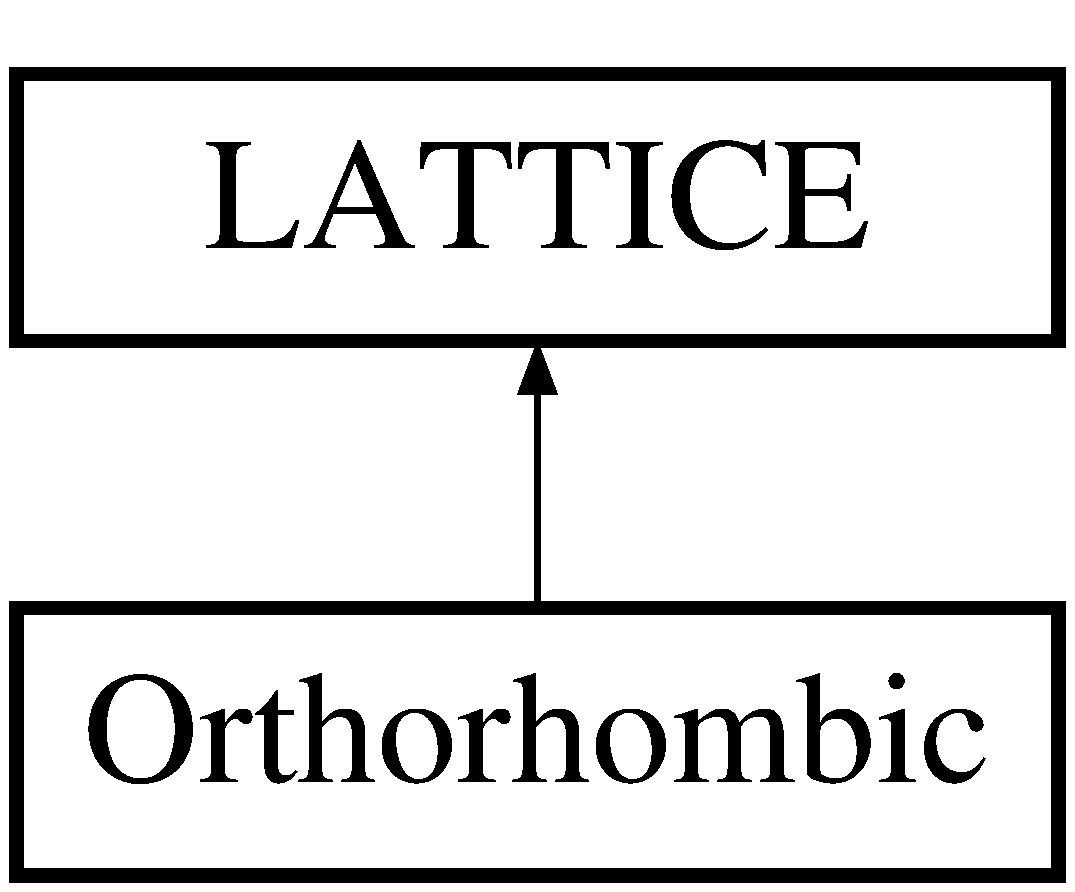
\includegraphics[height=2.000000cm]{class_orthorhombic}
\end{center}
\end{figure}
\subsection*{Public Member Functions}
\begin{DoxyCompactItemize}
\item 
\hyperlink{class_orthorhombic_a39f258370aaba742e7af9eb06fa15926}{Orthorhombic} (double i\+\_\+alat, double i\+\_\+blat, double i\+\_\+clat, char i\+\_\+lstyle\mbox{[}$\,$\mbox{]}, char $\ast$i\+\_\+element)
\begin{DoxyCompactList}\small\item\em Constructor for the \hyperlink{class_orthorhombic}{Orthorhombic} class when accessed from a gui session or when reading a parameters file. \end{DoxyCompactList}\item 
\hyperlink{class_orthorhombic_a36b36bb0a5fa04710aa934749fca1a21}{$\sim$\+Orthorhombic} ()
\end{DoxyCompactItemize}
\subsection*{Private Member Functions}
\begin{DoxyCompactItemize}
\item 
void \hyperlink{class_orthorhombic_ae95c1c0450eda0f01718ec52fec1a59c}{primitive} ()
\begin{DoxyCompactList}\small\item\em Defines lattice vectors, lattice parameters, and basis atoms for Simple \hyperlink{class_cubic}{Cubic}. \end{DoxyCompactList}\item 
void \hyperlink{class_orthorhombic_af7d8ab9b44633b12bf6d1f87554a8615}{B\+C\+C} ()
\begin{DoxyCompactList}\small\item\em Defines lattice vectors, lattice parameters, and basis atoms for Body Centered \hyperlink{class_cubic}{Cubic}. \end{DoxyCompactList}\item 
void \hyperlink{class_orthorhombic_af070eba51ade7d800bfc5adae33604e5}{F\+C\+C} ()
\begin{DoxyCompactList}\small\item\em Defines lattice vectors, lattice parameters, and basis atoms for Face Centered \hyperlink{class_cubic}{Cubic}. \end{DoxyCompactList}\end{DoxyCompactItemize}
\subsection*{Additional Inherited Members}


\subsection{Constructor \& Destructor Documentation}
\hypertarget{class_orthorhombic_a39f258370aaba742e7af9eb06fa15926}{}\index{Orthorhombic@{Orthorhombic}!Orthorhombic@{Orthorhombic}}
\index{Orthorhombic@{Orthorhombic}!Orthorhombic@{Orthorhombic}}
\subsubsection[{Orthorhombic}]{\setlength{\rightskip}{0pt plus 5cm}Orthorhombic\+::\+Orthorhombic (
\begin{DoxyParamCaption}
\item[{double}]{i\+\_\+alat, }
\item[{double}]{i\+\_\+blat, }
\item[{double}]{i\+\_\+clat, }
\item[{char}]{i\+\_\+lstyle\mbox{[}$\,$\mbox{]}, }
\item[{char $\ast$}]{i\+\_\+element}
\end{DoxyParamCaption}
)}\label{class_orthorhombic_a39f258370aaba742e7af9eb06fa15926}


Constructor for the \hyperlink{class_orthorhombic}{Orthorhombic} class when accessed from a gui session or when reading a parameters file. 


\begin{DoxyParams}[1]{Parameters}
\mbox{\tt in}  & {\em i\+\_\+alat} & -\/ lattice parameter for {\ttfamily a}, in Å \\
\hline
\mbox{\tt in}  & {\em i\+\_\+blat} & -\/ lattice parameter for {\ttfamily b}, in Å \\
\hline
\mbox{\tt in}  & {\em i\+\_\+clat} & -\/ lattice parameter for {\ttfamily c}, in Å \\
\hline
\mbox{\tt in}  & {\em i\+\_\+lstyle} & -\/ which cubic crystal style, \begin{DoxyItemize}
\item {\ttfamily S\+C}, {\ttfamily B\+C\+C}, {\ttfamily F\+C\+C} \end{DoxyItemize}
\\
\hline
\mbox{\tt in}  & {\em i\+\_\+element} & -\/ which element to assign to the crystal \\
\hline
\end{DoxyParams}
\hypertarget{class_orthorhombic_a36b36bb0a5fa04710aa934749fca1a21}{}\index{Orthorhombic@{Orthorhombic}!````~Orthorhombic@{$\sim$\+Orthorhombic}}
\index{````~Orthorhombic@{$\sim$\+Orthorhombic}!Orthorhombic@{Orthorhombic}}
\subsubsection[{$\sim$\+Orthorhombic}]{\setlength{\rightskip}{0pt plus 5cm}Orthorhombic\+::$\sim$\+Orthorhombic (
\begin{DoxyParamCaption}
{}
\end{DoxyParamCaption}
)}\label{class_orthorhombic_a36b36bb0a5fa04710aa934749fca1a21}


\subsection{Member Function Documentation}
\hypertarget{class_orthorhombic_af7d8ab9b44633b12bf6d1f87554a8615}{}\index{Orthorhombic@{Orthorhombic}!B\+C\+C@{B\+C\+C}}
\index{B\+C\+C@{B\+C\+C}!Orthorhombic@{Orthorhombic}}
\subsubsection[{B\+C\+C}]{\setlength{\rightskip}{0pt plus 5cm}void Orthorhombic\+::\+B\+C\+C (
\begin{DoxyParamCaption}
{}
\end{DoxyParamCaption}
)\hspace{0.3cm}{\ttfamily [private]}}\label{class_orthorhombic_af7d8ab9b44633b12bf6d1f87554a8615}


Defines lattice vectors, lattice parameters, and basis atoms for Body Centered \hyperlink{class_cubic}{Cubic}. 

\hypertarget{class_orthorhombic_af070eba51ade7d800bfc5adae33604e5}{}\index{Orthorhombic@{Orthorhombic}!F\+C\+C@{F\+C\+C}}
\index{F\+C\+C@{F\+C\+C}!Orthorhombic@{Orthorhombic}}
\subsubsection[{F\+C\+C}]{\setlength{\rightskip}{0pt plus 5cm}void Orthorhombic\+::\+F\+C\+C (
\begin{DoxyParamCaption}
{}
\end{DoxyParamCaption}
)\hspace{0.3cm}{\ttfamily [private]}}\label{class_orthorhombic_af070eba51ade7d800bfc5adae33604e5}


Defines lattice vectors, lattice parameters, and basis atoms for Face Centered \hyperlink{class_cubic}{Cubic}. 

\hypertarget{class_orthorhombic_ae95c1c0450eda0f01718ec52fec1a59c}{}\index{Orthorhombic@{Orthorhombic}!primitive@{primitive}}
\index{primitive@{primitive}!Orthorhombic@{Orthorhombic}}
\subsubsection[{primitive}]{\setlength{\rightskip}{0pt plus 5cm}void Orthorhombic\+::primitive (
\begin{DoxyParamCaption}
{}
\end{DoxyParamCaption}
)\hspace{0.3cm}{\ttfamily [private]}}\label{class_orthorhombic_ae95c1c0450eda0f01718ec52fec1a59c}


Defines lattice vectors, lattice parameters, and basis atoms for Simple \hyperlink{class_cubic}{Cubic}. 



The documentation for this class was generated from the following file\+:\begin{DoxyCompactItemize}
\item 
src/structures/\hyperlink{orthorhombic_8h}{orthorhombic.\+h}\end{DoxyCompactItemize}

\hypertarget{class_parser}{}\section{Parser Class Reference}
\label{class_parser}\index{Parser@{Parser}}


\subsection{Detailed Description}
\subsection*{{\bfseries Purpose\+:} }

\begin{DoxyVerb}/*****************************************************************************\
/  Class to process different types of strings, mainly conversion and search  \
/  functions.                                                                 \
/                                                                             \
/*****************************************************************************\
\end{DoxyVerb}


\begin{DoxyAuthor}{Author}
Joseph M. Gonzalez
\end{DoxyAuthor}
\begin{DoxyVersion}{Version}
0.\+1
\end{DoxyVersion}
\begin{DoxyDate}{Date}
Sep 13, 2015 19\+:16\+:20
\end{DoxyDate}
{\bfseries Contact} ~\newline
 \href{mailto:jmgonza6@mail.usf.edu}{\tt jmgonza6@mail.\+usf.\+edu} \subsection*{Public Member Functions}
\begin{DoxyCompactItemize}
\item 
\hyperlink{class_parser_a12234f6cd36b61af4b50c94a179422c1}{Parser} ()
\item 
\hyperlink{class_parser_a3e658b5917a93a3ef648050d060e3a93}{$\sim$\+Parser} ()
\item 
{\footnotesize template$<$typename ret\+Val $>$ }\\ret\+Val \hyperlink{class_parser_a7fd979d81465947482756e449939cc86}{str2num} (const std\+::string \&numstr)
\begin{DoxyCompactList}\small\item\em Template to convert a {\bfseries {\ttfamily std\+::string}} type to a numeric type. \end{DoxyCompactList}\item 
char $\ast$ \hyperlink{class_parser_ac9491abb25649667d76cce465f5e83e3}{str2char} (std\+::string str)
\begin{DoxyCompactList}\small\item\em Converts a {\bfseries {\ttfamily std\+::string}} type to {\bfseries {\ttfamily char} $\ast$} \end{DoxyCompactList}\item 
int \hyperlink{class_parser_af09b8e0fbda4e0c5a4d54aa8bebb0af4}{match\+\_\+phrase} (F\+I\+L\+E $\ast$fptr, char $\ast$phrase, char $\ast$line)
\begin{DoxyCompactList}\small\item\em Search for a specific pattern in a text file. \end{DoxyCompactList}\item 
int \hyperlink{class_parser_a70a6ed79f6a59e99d232c62002b0f1d0}{count\+\_\+words} (std\+::string list)
\begin{DoxyCompactList}\small\item\em Count the number of words in a string. \end{DoxyCompactList}\item 
int \hyperlink{class_parser_aa2f8f6e7b9906302de1d36b30bc9d969}{find\+\_\+rec} (std\+::string list, std\+::string pattern, int \&index)
\begin{DoxyCompactList}\small\item\em Find a word in a list of words separated by whitespace. \end{DoxyCompactList}\item 
std\+::vector$<$ std\+::string $>$ \hyperlink{class_parser_a9b2186ca0eff614eac41bc485ba06dd1}{split\+\_\+list} (std\+::string list, char delim)
\begin{DoxyCompactList}\small\item\em Parse a string of words based on a delimeter. \end{DoxyCompactList}\item 
char $\ast$ \hyperlink{class_parser_af5557acf700265e52c44d4501b90dbc3}{str\+\_\+manip} (char $\ast$str, char $\ast$insert, char delim)
\begin{DoxyCompactList}\small\item\em Insert a word based on a delimeter. \end{DoxyCompactList}\item 
int \hyperlink{class_parser_abf72a3b9424e25b2768a16bce23584c2}{get\+\_\+substrings} (std\+::string list, char d1, char d2, std\+::vector$<$ std\+::string $>$ \&keys, std\+::vector$<$ std\+::string $>$ \&vals)
\begin{DoxyCompactList}\small\item\em Parse a string of words based on two delimeters. \end{DoxyCompactList}\end{DoxyCompactItemize}


\subsection{Constructor \& Destructor Documentation}
\hypertarget{class_parser_a12234f6cd36b61af4b50c94a179422c1}{}\index{Parser@{Parser}!Parser@{Parser}}
\index{Parser@{Parser}!Parser@{Parser}}
\subsubsection[{Parser}]{\setlength{\rightskip}{0pt plus 5cm}Parser\+::\+Parser (
\begin{DoxyParamCaption}
{}
\end{DoxyParamCaption}
)}\label{class_parser_a12234f6cd36b61af4b50c94a179422c1}
\hypertarget{class_parser_a3e658b5917a93a3ef648050d060e3a93}{}\index{Parser@{Parser}!````~Parser@{$\sim$\+Parser}}
\index{````~Parser@{$\sim$\+Parser}!Parser@{Parser}}
\subsubsection[{$\sim$\+Parser}]{\setlength{\rightskip}{0pt plus 5cm}Parser\+::$\sim$\+Parser (
\begin{DoxyParamCaption}
{}
\end{DoxyParamCaption}
)}\label{class_parser_a3e658b5917a93a3ef648050d060e3a93}


\subsection{Member Function Documentation}
\hypertarget{class_parser_a70a6ed79f6a59e99d232c62002b0f1d0}{}\index{Parser@{Parser}!count\+\_\+words@{count\+\_\+words}}
\index{count\+\_\+words@{count\+\_\+words}!Parser@{Parser}}
\subsubsection[{count\+\_\+words}]{\setlength{\rightskip}{0pt plus 5cm}int Parser\+::count\+\_\+words (
\begin{DoxyParamCaption}
\item[{std\+::string}]{list}
\end{DoxyParamCaption}
)}\label{class_parser_a70a6ed79f6a59e99d232c62002b0f1d0}


Count the number of words in a string. 


\begin{DoxyParams}[1]{Parameters}
\mbox{\tt in}  & {\em list} & -\/ strings to be parsed based on whitespace \\
\hline
\end{DoxyParams}
\begin{DoxyReturn}{Returns}
number of words 
\end{DoxyReturn}
\hypertarget{class_parser_aa2f8f6e7b9906302de1d36b30bc9d969}{}\index{Parser@{Parser}!find\+\_\+rec@{find\+\_\+rec}}
\index{find\+\_\+rec@{find\+\_\+rec}!Parser@{Parser}}
\subsubsection[{find\+\_\+rec}]{\setlength{\rightskip}{0pt plus 5cm}int Parser\+::find\+\_\+rec (
\begin{DoxyParamCaption}
\item[{std\+::string}]{list, }
\item[{std\+::string}]{pattern, }
\item[{int \&}]{index}
\end{DoxyParamCaption}
)}\label{class_parser_aa2f8f6e7b9906302de1d36b30bc9d969}


Find a word in a list of words separated by whitespace. 


\begin{DoxyParams}[1]{Parameters}
\mbox{\tt in}  & {\em list} & -\/ string of words to be parsed \\
\hline
\mbox{\tt in}  & {\em pattern} & -\/ pattern to match in {\ttfamily list} \\
\hline
\mbox{\tt out}  & {\em index} & -\/ strings to be parsed based on whitespace \\
\hline
\end{DoxyParams}
\begin{DoxyReturn}{Returns}
{\bfseries {\ttfamily 1}} if successful, {\bfseries {\ttfamily 0}} otherwise. 
\end{DoxyReturn}
\hypertarget{class_parser_abf72a3b9424e25b2768a16bce23584c2}{}\index{Parser@{Parser}!get\+\_\+substrings@{get\+\_\+substrings}}
\index{get\+\_\+substrings@{get\+\_\+substrings}!Parser@{Parser}}
\subsubsection[{get\+\_\+substrings}]{\setlength{\rightskip}{0pt plus 5cm}int Parser\+::get\+\_\+substrings (
\begin{DoxyParamCaption}
\item[{std\+::string}]{list, }
\item[{char}]{d1, }
\item[{char}]{d2, }
\item[{std\+::vector$<$ std\+::string $>$ \&}]{keys, }
\item[{std\+::vector$<$ std\+::string $>$ \&}]{vals}
\end{DoxyParamCaption}
)}\label{class_parser_abf72a3b9424e25b2768a16bce23584c2}


Parse a string of words based on two delimeters. 


\begin{DoxyParams}[1]{Parameters}
\mbox{\tt in}  & {\em list} & -\/ string of words to be parsed \\
\hline
\mbox{\tt in}  & {\em d1} & -\/ fisrt delimeter to use for splitting \\
\hline
\mbox{\tt in}  & {\em d2} & -\/ second delimeter to use for splitting the result of {\ttfamily d1} \\
\hline
\mbox{\tt in}  & {\em keys} & -\/ keywords to search for in {\ttfamily list} \\
\hline
\mbox{\tt in}  & {\em vals} & -\/ values associated with {\ttfamily keys} in {\ttfamily list} \\
\hline
\end{DoxyParams}
\begin{DoxyReturn}{Returns}
{\bfseries {\ttfamily 1}} if successful, {\bfseries {\ttfamily 0}} otherwise. 
\end{DoxyReturn}
\hypertarget{class_parser_af09b8e0fbda4e0c5a4d54aa8bebb0af4}{}\index{Parser@{Parser}!match\+\_\+phrase@{match\+\_\+phrase}}
\index{match\+\_\+phrase@{match\+\_\+phrase}!Parser@{Parser}}
\subsubsection[{match\+\_\+phrase}]{\setlength{\rightskip}{0pt plus 5cm}int Parser\+::match\+\_\+phrase (
\begin{DoxyParamCaption}
\item[{F\+I\+L\+E $\ast$}]{fptr, }
\item[{char $\ast$}]{phrase, }
\item[{char $\ast$}]{line}
\end{DoxyParamCaption}
)}\label{class_parser_af09b8e0fbda4e0c5a4d54aa8bebb0af4}


Search for a specific pattern in a text file. 


\begin{DoxyParams}[1]{Parameters}
\mbox{\tt in}  & {\em fptr} & -\/ Pointer to the file \\
\hline
\mbox{\tt in}  & {\em phrase} & -\/ Specific pattern to match \\
\hline
\mbox{\tt out}  & {\em line} & -\/ Entire line containing the pattern, simillar to {\ttfamily grep} \\
\hline
\end{DoxyParams}
\begin{DoxyReturn}{Returns}
{\bfseries {\ttfamily 1}} if successful, {\bfseries {\ttfamily 0}} otherwise 
\end{DoxyReturn}
\hypertarget{class_parser_a9b2186ca0eff614eac41bc485ba06dd1}{}\index{Parser@{Parser}!split\+\_\+list@{split\+\_\+list}}
\index{split\+\_\+list@{split\+\_\+list}!Parser@{Parser}}
\subsubsection[{split\+\_\+list}]{\setlength{\rightskip}{0pt plus 5cm}std\+::vector$<$std\+::string$>$ Parser\+::split\+\_\+list (
\begin{DoxyParamCaption}
\item[{std\+::string}]{list, }
\item[{char}]{delim}
\end{DoxyParamCaption}
)}\label{class_parser_a9b2186ca0eff614eac41bc485ba06dd1}


Parse a string of words based on a delimeter. 


\begin{DoxyParams}[1]{Parameters}
\mbox{\tt in}  & {\em list} & -\/ string of words to be parsed \\
\hline
\mbox{\tt in}  & {\em delim} & -\/ delimeter to use for splitting \\
\hline
\end{DoxyParams}
\begin{DoxyReturn}{Returns}
a {\bfseries {\ttfamily std\+::vector$<$std\+::string$>$}} type containing the words found in {\ttfamily list} 
\end{DoxyReturn}
\hypertarget{class_parser_ac9491abb25649667d76cce465f5e83e3}{}\index{Parser@{Parser}!str2char@{str2char}}
\index{str2char@{str2char}!Parser@{Parser}}
\subsubsection[{str2char}]{\setlength{\rightskip}{0pt plus 5cm}char$\ast$ Parser\+::str2char (
\begin{DoxyParamCaption}
\item[{std\+::string}]{str}
\end{DoxyParamCaption}
)}\label{class_parser_ac9491abb25649667d76cce465f5e83e3}


Converts a {\bfseries {\ttfamily std\+::string}} type to {\bfseries {\ttfamily char} $\ast$} 


\begin{DoxyParams}[1]{Parameters}
\mbox{\tt in}  & {\em str} & -\/ the string to be converted \\
\hline
\end{DoxyParams}
\begin{DoxyReturn}{Returns}
{\bfseries {\ttfamily char} $\ast$} if successfull, {\bfseries {\ttfamily N\+U\+L\+L}} otherwise 
\end{DoxyReturn}
\hypertarget{class_parser_a7fd979d81465947482756e449939cc86}{}\index{Parser@{Parser}!str2num@{str2num}}
\index{str2num@{str2num}!Parser@{Parser}}
\subsubsection[{str2num}]{\setlength{\rightskip}{0pt plus 5cm}template$<$typename ret\+Val $>$ ret\+Val Parser\+::str2num (
\begin{DoxyParamCaption}
\item[{const std\+::string \&}]{numstr}
\end{DoxyParamCaption}
)\hspace{0.3cm}{\ttfamily [inline]}}\label{class_parser_a7fd979d81465947482756e449939cc86}


Template to convert a {\bfseries {\ttfamily std\+::string}} type to a numeric type. 


\begin{DoxyTemplParams}{Template Parameters}
{\em numstr} & -\/ Address of the string to convert \\
\hline
\end{DoxyTemplParams}
\begin{DoxyReturn}{Returns}
a number of type {\bfseries {\ttfamily ret\+Val}} 
\end{DoxyReturn}
\hypertarget{class_parser_af5557acf700265e52c44d4501b90dbc3}{}\index{Parser@{Parser}!str\+\_\+manip@{str\+\_\+manip}}
\index{str\+\_\+manip@{str\+\_\+manip}!Parser@{Parser}}
\subsubsection[{str\+\_\+manip}]{\setlength{\rightskip}{0pt plus 5cm}char$\ast$ Parser\+::str\+\_\+manip (
\begin{DoxyParamCaption}
\item[{char $\ast$}]{str, }
\item[{char $\ast$}]{insert, }
\item[{char}]{delim}
\end{DoxyParamCaption}
)}\label{class_parser_af5557acf700265e52c44d4501b90dbc3}


Insert a word based on a delimeter. 


\begin{DoxyParams}[1]{Parameters}
\mbox{\tt in}  & {\em str} & -\/ string to have a word inserted \\
\hline
\mbox{\tt in}  & {\em insert} & -\/ word to insert in {\ttfamily str} \\
\hline
\mbox{\tt in}  & {\em delim} & -\/ delimeter to use for locating the end \\
\hline
\end{DoxyParams}
\begin{DoxyReturn}{Returns}
a {\bfseries {\ttfamily char$\ast$}} type containing compound word 
\end{DoxyReturn}


The documentation for this class was generated from the following file\+:\begin{DoxyCompactItemize}
\item 
src/util/\hyperlink{common_8h}{common.\+h}\end{DoxyCompactItemize}

\hypertarget{struct_periodic_table}{}\section{Periodic\+Table Struct Reference}
\label{struct_periodic_table}\index{Periodic\+Table@{Periodic\+Table}}


A structure containing strings representing up to element 110 and their associated masses in A\+M\+U.  




\subsection{Detailed Description}
A structure containing strings representing up to element 110 and their associated masses in A\+M\+U. \subsection*{Data Fields}
\begin{DoxyCompactItemize}
\item 
std\+::string \hyperlink{struct_periodic_table_ab11add4b0907eeaabe309791f8c2a4a4}{elements} \mbox{[}110\mbox{]}
\item 
double \hyperlink{struct_periodic_table_a8932a977c48df97676a3e85830c9e855}{amu} \mbox{[}110\mbox{]}
\end{DoxyCompactItemize}


\subsection{Field Documentation}
\hypertarget{struct_periodic_table_a8932a977c48df97676a3e85830c9e855}{}\index{Periodic\+Table@{Periodic\+Table}!amu@{amu}}
\index{amu@{amu}!Periodic\+Table@{Periodic\+Table}}
\subsubsection[{amu}]{\setlength{\rightskip}{0pt plus 5cm}double Periodic\+Table\+::amu\mbox{[}110\mbox{]}}\label{struct_periodic_table_a8932a977c48df97676a3e85830c9e855}
\hypertarget{struct_periodic_table_ab11add4b0907eeaabe309791f8c2a4a4}{}\index{Periodic\+Table@{Periodic\+Table}!elements@{elements}}
\index{elements@{elements}!Periodic\+Table@{Periodic\+Table}}
\subsubsection[{elements}]{\setlength{\rightskip}{0pt plus 5cm}std\+::string Periodic\+Table\+::elements\mbox{[}110\mbox{]}}\label{struct_periodic_table_ab11add4b0907eeaabe309791f8c2a4a4}


The documentation for this struct was generated from the following file\+:\begin{DoxyCompactItemize}
\item 
src/util/\hyperlink{common_8h}{common.\+h}\end{DoxyCompactItemize}

\hypertarget{struct_point}{}\section{Point Struct Reference}
\label{struct_point}\index{Point@{Point}}


x,y,z coordinates for a point in space  




\subsection{Detailed Description}
x,y,z coordinates for a point in space \subsection*{Data Fields}
\begin{DoxyCompactItemize}
\item 
float \hyperlink{struct_point_a59432b14c29b6596fc812ad6dc308137}{x} \mbox{[}3\mbox{]}
\item 
float \hyperlink{struct_point_a1e9f90253cb5724ee72043b9e3469d04}{n} \mbox{[}3\mbox{]}
\end{DoxyCompactItemize}


\subsection{Field Documentation}
\hypertarget{struct_point_a1e9f90253cb5724ee72043b9e3469d04}{}\index{Point@{Point}!n@{n}}
\index{n@{n}!Point@{Point}}
\subsubsection[{n}]{\setlength{\rightskip}{0pt plus 5cm}float Point\+::n\mbox{[}3\mbox{]}}\label{struct_point_a1e9f90253cb5724ee72043b9e3469d04}
\hypertarget{struct_point_a59432b14c29b6596fc812ad6dc308137}{}\index{Point@{Point}!x@{x}}
\index{x@{x}!Point@{Point}}
\subsubsection[{x}]{\setlength{\rightskip}{0pt plus 5cm}float Point\+::x\mbox{[}3\mbox{]}}\label{struct_point_a59432b14c29b6596fc812ad6dc308137}


The documentation for this struct was generated from the following file\+:\begin{DoxyCompactItemize}
\item 
src/util/\hyperlink{common_8h}{common.\+h}\end{DoxyCompactItemize}

\hypertarget{class_reader}{}\section{Reader Class Reference}
\label{class_reader}\index{Reader@{Reader}}


\subsection{Detailed Description}
\subsection*{{\bfseries Purpose\+:} }

\begin{DoxyVerb}/********************************************************************************\
/  Class for reading crystal parameters from a file                              \
/                                                                                \
/********************************************************************************\
\end{DoxyVerb}


\begin{DoxyAuthor}{Author}
Joseph M. Gonzalez
\end{DoxyAuthor}
\begin{DoxyVersion}{Version}
0.\+1
\end{DoxyVersion}
\begin{DoxyDate}{Date}
Sep 27, 2015 23\+:16\+:20
\end{DoxyDate}
{\bfseries Contact} ~\newline
 \href{mailto:jmgonza6@mail.usf.edu}{\tt jmgonza6@mail.\+usf.\+edu} \subsection*{Public Member Functions}
\begin{DoxyCompactItemize}
\item 
\hyperlink{class_reader_adcda31b507720ab44044d7a21686fba2}{Reader} ()
\item 
\hyperlink{class_reader_a78089542fd27a0ac2df6702fffe8725c}{$\sim$\+Reader} ()
\item 
void \hyperlink{class_reader_afae5e105c093f58c13a558bc92fc7618}{file} (char $\ast$pf)
\item 
int \hyperlink{class_reader_a1967f81a208b23983d13ff8c72d453ca}{insane} ()
\end{DoxyCompactItemize}
\subsection*{Data Fields}
\begin{DoxyCompactItemize}
\item 
double \hyperlink{class_reader_ae27e67c8d78fb8fac565ec079529b589}{alat}
\begin{DoxyCompactList}\small\item\em latttice parameter a (Å) \end{DoxyCompactList}\item 
double \hyperlink{class_reader_a8e2240f9ad9a7c1423e0888e474f4c9e}{blat}
\begin{DoxyCompactList}\small\item\em lattice parameter b (Å) \end{DoxyCompactList}\item 
double \hyperlink{class_reader_ad10c6e643d5cb651bed0c96790099b51}{clat}
\begin{DoxyCompactList}\small\item\em lattice parameter c (Å) \end{DoxyCompactList}\item 
double \hyperlink{class_reader_a421cb70a4a8746a68fe2618ed597c5a0}{alpha}
\begin{DoxyCompactList}\small\item\em angle beteween c \& b \end{DoxyCompactList}\item 
double \hyperlink{class_reader_a47234e1e633f932334c4304cf01824a1}{beta}
\begin{DoxyCompactList}\small\item\em angle between c \& a \end{DoxyCompactList}\item 
double \hyperlink{class_reader_ab2127a4e365fd3528c017a76375d60c4}{gamma}
\begin{DoxyCompactList}\small\item\em angle between a \& b \end{DoxyCompactList}\item 
double \hyperlink{class_reader_a6eb90d21148a08f9ef4e3dc478917d63}{cta}
\begin{DoxyCompactList}\small\item\em c/a ratio, for use with Hexagonal(), h-\/\+B\+N(), Graphene() \end{DoxyCompactList}\item 
int \hyperlink{class_reader_afd2686bb2f2f9eec9601287385d7159e}{lbasis}
\begin{DoxyCompactList}\small\item\em number of basis atoms for graphene \end{DoxyCompactList}\item 
int \hyperlink{class_reader_a85d35ff338db8e5915d7620a730df6fb}{nx}
\begin{DoxyCompactList}\small\item\em supercell dimension along x \end{DoxyCompactList}\item 
int \hyperlink{class_reader_a68ce806c514dd9323b66de3ca25285c2}{ny}
\begin{DoxyCompactList}\small\item\em supercell dimension along y \end{DoxyCompactList}\item 
int \hyperlink{class_reader_ab09026e1e834afa843386f8da4f3e5d3}{nz}
\begin{DoxyCompactList}\small\item\em supercell dimension along z \end{DoxyCompactList}\item 
int \hyperlink{class_reader_a913c9024181fd0fbb2dea5265fa097c1}{fractional}
\begin{DoxyCompactList}\small\item\em fractional coordinates, 1 = true, 0 = false \end{DoxyCompactList}\item 
int \hyperlink{class_reader_aa0c8ca660b7982ecc0fcaa673a1db16b}{graphene}
\begin{DoxyCompactList}\small\item\em graphene structure was built, 1 = true, 0 = false \end{DoxyCompactList}\item 
int \hyperlink{class_reader_aeffa187da9ac5feb5c3e5e078fe43fde}{custom}
\begin{DoxyCompactList}\small\item\em a custom structure was built, 1 = true, 0 = false \end{DoxyCompactList}\item 
int \hyperlink{class_reader_a3a38a2290db448491a46a74ca4413c71}{resets}
\begin{DoxyCompactList}\small\item\em reset count \end{DoxyCompactList}\item 
int \hyperlink{class_reader_a7915928dbe39a87fe9d7ef829f848acb}{run\+\_\+count}
\begin{DoxyCompactList}\small\item\em run count, for debugging \end{DoxyCompactList}\item 
int \hyperlink{class_reader_ada4132c63c686a21ea6eb8f05d724edc}{quit}
\begin{DoxyCompactList}\small\item\em quit signal \end{DoxyCompactList}\item 
int \hyperlink{class_reader_a4686a622a101960a17a1786a45b84bcd}{view}
\begin{DoxyCompactList}\small\item\em render+build signal \end{DoxyCompactList}\item 
char $\ast$ \hyperlink{class_reader_a2aa3818b76e5565fef7e72a5018ca084}{pfile}
\begin{DoxyCompactList}\small\item\em parameter file to define the crystal \end{DoxyCompactList}\item 
char $\ast$ \hyperlink{class_reader_a05d97010d814f91cffe66657e2c39ffd}{out\+\_\+name}
\begin{DoxyCompactList}\small\item\em file name to write \end{DoxyCompactList}\item 
char $\ast$ \hyperlink{class_reader_a8031979223c6835ee2a52be58c13f9b1}{file\+\_\+format}
\begin{DoxyCompactList}\small\item\em type of file to write \end{DoxyCompactList}\item 
char $\ast$ \hyperlink{class_reader_a9aa6c187535ed940397c836aacfcc0c1}{bravais}
\begin{DoxyCompactList}\small\item\em which lattice ? \end{DoxyCompactList}\item 
char $\ast$ \hyperlink{class_reader_aaaa3ec196647f9d79f39fac3db21d288}{lstyle}
\begin{DoxyCompactList}\small\item\em bravais lattice style, B\+C\+C \end{DoxyCompactList}\item 
char $\ast$ \hyperlink{class_reader_aa1f260272da17a496f1ecd3ce39281b9}{pd\+\_\+struct}
\begin{DoxyCompactList}\small\item\em defines a library structure to use \end{DoxyCompactList}\item 
char $\ast$ \hyperlink{class_reader_aad797cfb4296c19561d2729de8cd9333}{element}
\begin{DoxyCompactList}\small\item\em which species ? \end{DoxyCompactList}\item 
std\+::vector$<$ std\+::string $>$ \hyperlink{class_reader_a81df051804ba55004944e2d6f9a43cf7}{elem\+List}
\begin{DoxyCompactList}\small\item\em define a custom stoichiometry (C,H,N,O) \end{DoxyCompactList}\item 
std\+::vector$<$ int $>$ \hyperlink{class_reader_a81393d6441793db4fd62c7a4652518d3}{elem\+Count}
\begin{DoxyCompactList}\small\item\em define a custom stoichiometry (2,4,1,3) \end{DoxyCompactList}\item 
std\+::vector$<$ std\+::vector$<$ double $>$ $>$ \hyperlink{class_reader_a5f34996abadc7f998ffd1c34c4cfb380}{custom\+Basis}
\begin{DoxyCompactList}\small\item\em container for defining a custom basis set \end{DoxyCompactList}\item 
std\+::string \hyperlink{class_reader_a5cad9d6f8773e4ca9e6ae63b4dd7a307}{custom\+Name}
\begin{DoxyCompactList}\small\item\em chemical formula of a custom structure \end{DoxyCompactList}\item 
\hyperlink{class_parser}{Parser} $\ast$ \hyperlink{class_reader_a4a2ce1dccacd1cb00f0a226f4f78c9d6}{parser}
\end{DoxyCompactItemize}


\subsection{Constructor \& Destructor Documentation}
\hypertarget{class_reader_adcda31b507720ab44044d7a21686fba2}{}\index{Reader@{Reader}!Reader@{Reader}}
\index{Reader@{Reader}!Reader@{Reader}}
\subsubsection[{Reader}]{\setlength{\rightskip}{0pt plus 5cm}Reader\+::\+Reader (
\begin{DoxyParamCaption}
{}
\end{DoxyParamCaption}
)}\label{class_reader_adcda31b507720ab44044d7a21686fba2}
\hypertarget{class_reader_a78089542fd27a0ac2df6702fffe8725c}{}\index{Reader@{Reader}!````~Reader@{$\sim$\+Reader}}
\index{````~Reader@{$\sim$\+Reader}!Reader@{Reader}}
\subsubsection[{$\sim$\+Reader}]{\setlength{\rightskip}{0pt plus 5cm}Reader\+::$\sim$\+Reader (
\begin{DoxyParamCaption}
{}
\end{DoxyParamCaption}
)}\label{class_reader_a78089542fd27a0ac2df6702fffe8725c}


\subsection{Member Function Documentation}
\hypertarget{class_reader_afae5e105c093f58c13a558bc92fc7618}{}\index{Reader@{Reader}!file@{file}}
\index{file@{file}!Reader@{Reader}}
\subsubsection[{file}]{\setlength{\rightskip}{0pt plus 5cm}void Reader\+::file (
\begin{DoxyParamCaption}
\item[{char $\ast$}]{pf}
\end{DoxyParamCaption}
)}\label{class_reader_afae5e105c093f58c13a558bc92fc7618}
\hypertarget{class_reader_a1967f81a208b23983d13ff8c72d453ca}{}\index{Reader@{Reader}!insane@{insane}}
\index{insane@{insane}!Reader@{Reader}}
\subsubsection[{insane}]{\setlength{\rightskip}{0pt plus 5cm}int Reader\+::insane (
\begin{DoxyParamCaption}
{}
\end{DoxyParamCaption}
)}\label{class_reader_a1967f81a208b23983d13ff8c72d453ca}


\subsection{Field Documentation}
\hypertarget{class_reader_ae27e67c8d78fb8fac565ec079529b589}{}\index{Reader@{Reader}!alat@{alat}}
\index{alat@{alat}!Reader@{Reader}}
\subsubsection[{alat}]{\setlength{\rightskip}{0pt plus 5cm}double Reader\+::alat}\label{class_reader_ae27e67c8d78fb8fac565ec079529b589}


latttice parameter a (Å) 

\hypertarget{class_reader_a421cb70a4a8746a68fe2618ed597c5a0}{}\index{Reader@{Reader}!alpha@{alpha}}
\index{alpha@{alpha}!Reader@{Reader}}
\subsubsection[{alpha}]{\setlength{\rightskip}{0pt plus 5cm}double Reader\+::alpha}\label{class_reader_a421cb70a4a8746a68fe2618ed597c5a0}


angle beteween c \& b 

\hypertarget{class_reader_a47234e1e633f932334c4304cf01824a1}{}\index{Reader@{Reader}!beta@{beta}}
\index{beta@{beta}!Reader@{Reader}}
\subsubsection[{beta}]{\setlength{\rightskip}{0pt plus 5cm}double Reader\+::beta}\label{class_reader_a47234e1e633f932334c4304cf01824a1}


angle between c \& a 

\hypertarget{class_reader_a8e2240f9ad9a7c1423e0888e474f4c9e}{}\index{Reader@{Reader}!blat@{blat}}
\index{blat@{blat}!Reader@{Reader}}
\subsubsection[{blat}]{\setlength{\rightskip}{0pt plus 5cm}double Reader\+::blat}\label{class_reader_a8e2240f9ad9a7c1423e0888e474f4c9e}


lattice parameter b (Å) 

\hypertarget{class_reader_a9aa6c187535ed940397c836aacfcc0c1}{}\index{Reader@{Reader}!bravais@{bravais}}
\index{bravais@{bravais}!Reader@{Reader}}
\subsubsection[{bravais}]{\setlength{\rightskip}{0pt plus 5cm}char$\ast$ Reader\+::bravais}\label{class_reader_a9aa6c187535ed940397c836aacfcc0c1}


which lattice ? 

\hypertarget{class_reader_ad10c6e643d5cb651bed0c96790099b51}{}\index{Reader@{Reader}!clat@{clat}}
\index{clat@{clat}!Reader@{Reader}}
\subsubsection[{clat}]{\setlength{\rightskip}{0pt plus 5cm}double Reader\+::clat}\label{class_reader_ad10c6e643d5cb651bed0c96790099b51}


lattice parameter c (Å) 

\hypertarget{class_reader_a6eb90d21148a08f9ef4e3dc478917d63}{}\index{Reader@{Reader}!cta@{cta}}
\index{cta@{cta}!Reader@{Reader}}
\subsubsection[{cta}]{\setlength{\rightskip}{0pt plus 5cm}double Reader\+::cta}\label{class_reader_a6eb90d21148a08f9ef4e3dc478917d63}


c/a ratio, for use with Hexagonal(), h-\/\+B\+N(), Graphene() 

\hypertarget{class_reader_aeffa187da9ac5feb5c3e5e078fe43fde}{}\index{Reader@{Reader}!custom@{custom}}
\index{custom@{custom}!Reader@{Reader}}
\subsubsection[{custom}]{\setlength{\rightskip}{0pt plus 5cm}int Reader\+::custom}\label{class_reader_aeffa187da9ac5feb5c3e5e078fe43fde}


a custom structure was built, 1 = true, 0 = false 

\hypertarget{class_reader_a5f34996abadc7f998ffd1c34c4cfb380}{}\index{Reader@{Reader}!custom\+Basis@{custom\+Basis}}
\index{custom\+Basis@{custom\+Basis}!Reader@{Reader}}
\subsubsection[{custom\+Basis}]{\setlength{\rightskip}{0pt plus 5cm}std\+::vector$<$std\+::vector$<$double$>$ $>$ Reader\+::custom\+Basis}\label{class_reader_a5f34996abadc7f998ffd1c34c4cfb380}


container for defining a custom basis set 

\hypertarget{class_reader_a5cad9d6f8773e4ca9e6ae63b4dd7a307}{}\index{Reader@{Reader}!custom\+Name@{custom\+Name}}
\index{custom\+Name@{custom\+Name}!Reader@{Reader}}
\subsubsection[{custom\+Name}]{\setlength{\rightskip}{0pt plus 5cm}std\+::string Reader\+::custom\+Name}\label{class_reader_a5cad9d6f8773e4ca9e6ae63b4dd7a307}


chemical formula of a custom structure 

\hypertarget{class_reader_a81393d6441793db4fd62c7a4652518d3}{}\index{Reader@{Reader}!elem\+Count@{elem\+Count}}
\index{elem\+Count@{elem\+Count}!Reader@{Reader}}
\subsubsection[{elem\+Count}]{\setlength{\rightskip}{0pt plus 5cm}std\+::vector$<$int$>$ Reader\+::elem\+Count}\label{class_reader_a81393d6441793db4fd62c7a4652518d3}


define a custom stoichiometry (2,4,1,3) 

\hypertarget{class_reader_aad797cfb4296c19561d2729de8cd9333}{}\index{Reader@{Reader}!element@{element}}
\index{element@{element}!Reader@{Reader}}
\subsubsection[{element}]{\setlength{\rightskip}{0pt plus 5cm}char$\ast$ Reader\+::element}\label{class_reader_aad797cfb4296c19561d2729de8cd9333}


which species ? 

\hypertarget{class_reader_a81df051804ba55004944e2d6f9a43cf7}{}\index{Reader@{Reader}!elem\+List@{elem\+List}}
\index{elem\+List@{elem\+List}!Reader@{Reader}}
\subsubsection[{elem\+List}]{\setlength{\rightskip}{0pt plus 5cm}std\+::vector$<$std\+::string$>$ Reader\+::elem\+List}\label{class_reader_a81df051804ba55004944e2d6f9a43cf7}


define a custom stoichiometry (C,H,N,O) 

\hypertarget{class_reader_a8031979223c6835ee2a52be58c13f9b1}{}\index{Reader@{Reader}!file\+\_\+format@{file\+\_\+format}}
\index{file\+\_\+format@{file\+\_\+format}!Reader@{Reader}}
\subsubsection[{file\+\_\+format}]{\setlength{\rightskip}{0pt plus 5cm}char$\ast$ Reader\+::file\+\_\+format}\label{class_reader_a8031979223c6835ee2a52be58c13f9b1}


type of file to write 

\hypertarget{class_reader_a913c9024181fd0fbb2dea5265fa097c1}{}\index{Reader@{Reader}!fractional@{fractional}}
\index{fractional@{fractional}!Reader@{Reader}}
\subsubsection[{fractional}]{\setlength{\rightskip}{0pt plus 5cm}int Reader\+::fractional}\label{class_reader_a913c9024181fd0fbb2dea5265fa097c1}


fractional coordinates, 1 = true, 0 = false 

\hypertarget{class_reader_ab2127a4e365fd3528c017a76375d60c4}{}\index{Reader@{Reader}!gamma@{gamma}}
\index{gamma@{gamma}!Reader@{Reader}}
\subsubsection[{gamma}]{\setlength{\rightskip}{0pt plus 5cm}double Reader\+::gamma}\label{class_reader_ab2127a4e365fd3528c017a76375d60c4}


angle between a \& b 

\hypertarget{class_reader_aa0c8ca660b7982ecc0fcaa673a1db16b}{}\index{Reader@{Reader}!graphene@{graphene}}
\index{graphene@{graphene}!Reader@{Reader}}
\subsubsection[{graphene}]{\setlength{\rightskip}{0pt plus 5cm}int Reader\+::graphene}\label{class_reader_aa0c8ca660b7982ecc0fcaa673a1db16b}


graphene structure was built, 1 = true, 0 = false 

\hypertarget{class_reader_afd2686bb2f2f9eec9601287385d7159e}{}\index{Reader@{Reader}!lbasis@{lbasis}}
\index{lbasis@{lbasis}!Reader@{Reader}}
\subsubsection[{lbasis}]{\setlength{\rightskip}{0pt plus 5cm}int Reader\+::lbasis}\label{class_reader_afd2686bb2f2f9eec9601287385d7159e}


number of basis atoms for graphene 

\hypertarget{class_reader_aaaa3ec196647f9d79f39fac3db21d288}{}\index{Reader@{Reader}!lstyle@{lstyle}}
\index{lstyle@{lstyle}!Reader@{Reader}}
\subsubsection[{lstyle}]{\setlength{\rightskip}{0pt plus 5cm}char$\ast$ Reader\+::lstyle}\label{class_reader_aaaa3ec196647f9d79f39fac3db21d288}


bravais lattice style, B\+C\+C 

\hypertarget{class_reader_a85d35ff338db8e5915d7620a730df6fb}{}\index{Reader@{Reader}!nx@{nx}}
\index{nx@{nx}!Reader@{Reader}}
\subsubsection[{nx}]{\setlength{\rightskip}{0pt plus 5cm}int Reader\+::nx}\label{class_reader_a85d35ff338db8e5915d7620a730df6fb}


supercell dimension along x 

\hypertarget{class_reader_a68ce806c514dd9323b66de3ca25285c2}{}\index{Reader@{Reader}!ny@{ny}}
\index{ny@{ny}!Reader@{Reader}}
\subsubsection[{ny}]{\setlength{\rightskip}{0pt plus 5cm}int Reader\+::ny}\label{class_reader_a68ce806c514dd9323b66de3ca25285c2}


supercell dimension along y 

\hypertarget{class_reader_ab09026e1e834afa843386f8da4f3e5d3}{}\index{Reader@{Reader}!nz@{nz}}
\index{nz@{nz}!Reader@{Reader}}
\subsubsection[{nz}]{\setlength{\rightskip}{0pt plus 5cm}int Reader\+::nz}\label{class_reader_ab09026e1e834afa843386f8da4f3e5d3}


supercell dimension along z 

\hypertarget{class_reader_a05d97010d814f91cffe66657e2c39ffd}{}\index{Reader@{Reader}!out\+\_\+name@{out\+\_\+name}}
\index{out\+\_\+name@{out\+\_\+name}!Reader@{Reader}}
\subsubsection[{out\+\_\+name}]{\setlength{\rightskip}{0pt plus 5cm}char$\ast$ Reader\+::out\+\_\+name}\label{class_reader_a05d97010d814f91cffe66657e2c39ffd}


file name to write 

\hypertarget{class_reader_a4a2ce1dccacd1cb00f0a226f4f78c9d6}{}\index{Reader@{Reader}!parser@{parser}}
\index{parser@{parser}!Reader@{Reader}}
\subsubsection[{parser}]{\setlength{\rightskip}{0pt plus 5cm}{\bf Parser}$\ast$ Reader\+::parser}\label{class_reader_a4a2ce1dccacd1cb00f0a226f4f78c9d6}
\hypertarget{class_reader_aa1f260272da17a496f1ecd3ce39281b9}{}\index{Reader@{Reader}!pd\+\_\+struct@{pd\+\_\+struct}}
\index{pd\+\_\+struct@{pd\+\_\+struct}!Reader@{Reader}}
\subsubsection[{pd\+\_\+struct}]{\setlength{\rightskip}{0pt plus 5cm}char$\ast$ Reader\+::pd\+\_\+struct}\label{class_reader_aa1f260272da17a496f1ecd3ce39281b9}


defines a library structure to use 

\hypertarget{class_reader_a2aa3818b76e5565fef7e72a5018ca084}{}\index{Reader@{Reader}!pfile@{pfile}}
\index{pfile@{pfile}!Reader@{Reader}}
\subsubsection[{pfile}]{\setlength{\rightskip}{0pt plus 5cm}char$\ast$ Reader\+::pfile}\label{class_reader_a2aa3818b76e5565fef7e72a5018ca084}


parameter file to define the crystal 

\hypertarget{class_reader_ada4132c63c686a21ea6eb8f05d724edc}{}\index{Reader@{Reader}!quit@{quit}}
\index{quit@{quit}!Reader@{Reader}}
\subsubsection[{quit}]{\setlength{\rightskip}{0pt plus 5cm}int Reader\+::quit}\label{class_reader_ada4132c63c686a21ea6eb8f05d724edc}


quit signal 

\hypertarget{class_reader_a3a38a2290db448491a46a74ca4413c71}{}\index{Reader@{Reader}!resets@{resets}}
\index{resets@{resets}!Reader@{Reader}}
\subsubsection[{resets}]{\setlength{\rightskip}{0pt plus 5cm}int Reader\+::resets}\label{class_reader_a3a38a2290db448491a46a74ca4413c71}


reset count 

\hypertarget{class_reader_a7915928dbe39a87fe9d7ef829f848acb}{}\index{Reader@{Reader}!run\+\_\+count@{run\+\_\+count}}
\index{run\+\_\+count@{run\+\_\+count}!Reader@{Reader}}
\subsubsection[{run\+\_\+count}]{\setlength{\rightskip}{0pt plus 5cm}int Reader\+::run\+\_\+count}\label{class_reader_a7915928dbe39a87fe9d7ef829f848acb}


run count, for debugging 

\hypertarget{class_reader_a4686a622a101960a17a1786a45b84bcd}{}\index{Reader@{Reader}!view@{view}}
\index{view@{view}!Reader@{Reader}}
\subsubsection[{view}]{\setlength{\rightskip}{0pt plus 5cm}int Reader\+::view}\label{class_reader_a4686a622a101960a17a1786a45b84bcd}


render+build signal 



The documentation for this class was generated from the following file\+:\begin{DoxyCompactItemize}
\item 
src/util/\hyperlink{reader_8h}{reader.\+h}\end{DoxyCompactItemize}

\hypertarget{class_structure_lib}{}\section{Structure\+Lib Class Reference}
\label{class_structure_lib}\index{Structure\+Lib@{Structure\+Lib}}


\subsection{Detailed Description}
\subsection*{{\bfseries Purpose\+:} }

\begin{DoxyVerb}/******************************************************************************\
/  Class to generate the basis atom positions, lattice vectors and lattice     \
/  parameters for various 2D materials  and Energetic materials, specifically, \
/  2D materials: Graphene, h-BN                                                \
/                MDC-2H/1T i.e.  (Pb,Sn)(S,Se,Te)2                             \
/                TMDC-2H/1T i.e. (Mo,W)(S,Se,Te)2                              \
/  Energetic materials: PETN-I, TATB, β-HMX                                    \
/                                                                              \
/  * * Inherits from the LATTICE class                                         \
/                                                                              \ 
/******************************************************************************\
\end{DoxyVerb}


\begin{DoxyAuthor}{Author}
Joseph M. Gonzalez
\end{DoxyAuthor}
\begin{DoxyVersion}{Version}
0.\+3
\end{DoxyVersion}
\begin{DoxyDate}{Date}
Sep 13, 2015 19\+:16\+:20
\end{DoxyDate}
{\bfseries Contact} ~\newline
 \href{mailto:jmgonza6@mail.usf.edu}{\tt jmgonza6@mail.\+usf.\+edu} Inheritance diagram for Structure\+Lib\+:\begin{figure}[H]
\begin{center}
\leavevmode
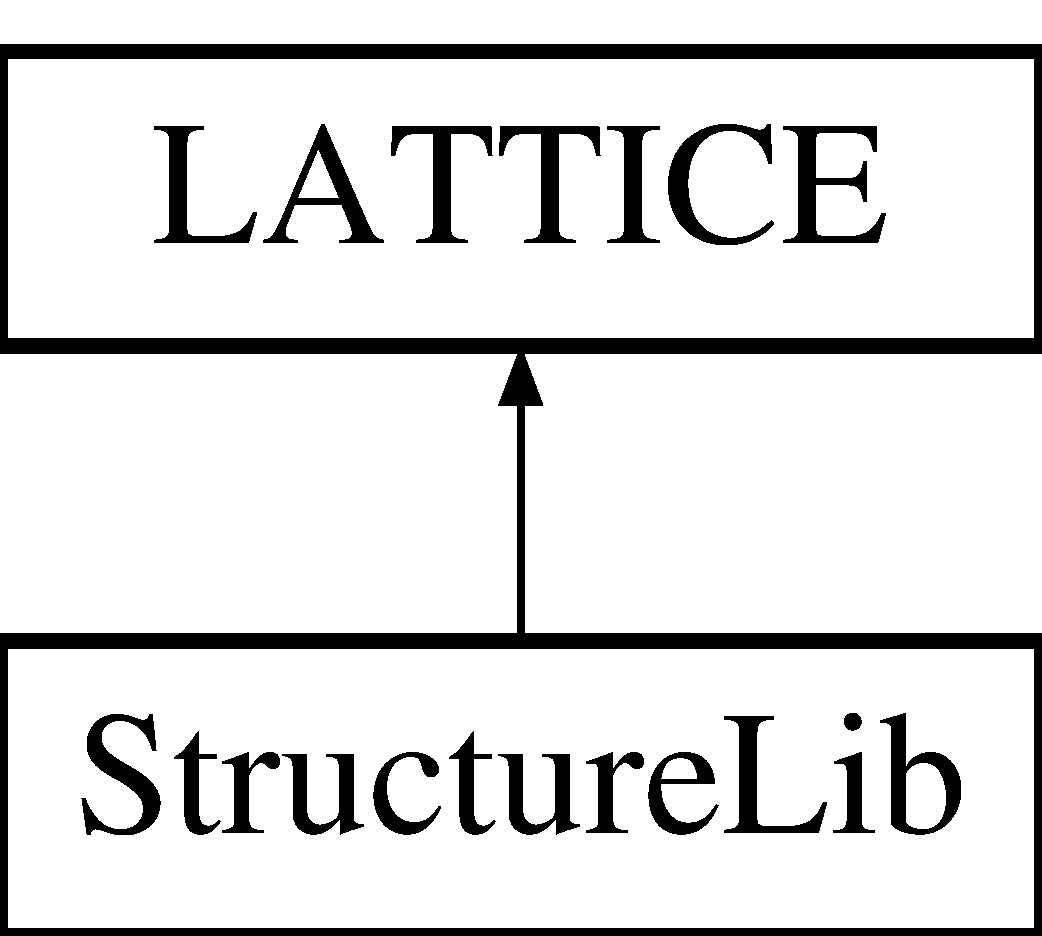
\includegraphics[height=2.000000cm]{class_structure_lib}
\end{center}
\end{figure}
\subsection*{Public Member Functions}
\begin{DoxyCompactItemize}
\item 
\hyperlink{class_structure_lib_a502fa21baaf8178d3863394a449e85d3}{Structure\+Lib} (char i\+\_\+lstyle\mbox{[}$\,$\mbox{]}, int basis\+Atoms, double i\+\_\+alat, double i\+\_\+clat, std\+::vector$<$ std\+::string $>$ elements)
\begin{DoxyCompactList}\small\item\em Constructor for the graphene class when accessed from a gui session or when reading a parameters file. \end{DoxyCompactList}\item 
\hyperlink{class_structure_lib_a40fe5cf7ef632df96ef10c523926ee44}{$\sim$\+Structure\+Lib} ()
\end{DoxyCompactItemize}
\subsection*{Private Member Functions}
\begin{DoxyCompactItemize}
\item 
void \hyperlink{class_structure_lib_ac4e830377b5c9b60761deb8feb00dbce}{graphene} (double i\+\_\+alat, double i\+\_\+clat, int basis\+Atoms)
\begin{DoxyCompactList}\small\item\em Constrct an hexagonal 2 atom unit cell or a 4 atom rectangular unit cell. \end{DoxyCompactList}\item 
void \hyperlink{class_structure_lib_a0b668498d5600cc7ec3da71f0b7cc9a4}{h\+\_\+bn} ()
\begin{DoxyCompactList}\small\item\em Define the basis atoms and lattice for hexagonal Boron Nitride. \end{DoxyCompactList}\item 
void \hyperlink{class_structure_lib_a08e109e6475bf16b14041341e05de271}{mdc\+\_\+2h} (double i\+\_\+alat, double i\+\_\+clat, std\+::vector$<$ std\+::string $>$ elements)
\begin{DoxyCompactList}\small\item\em Define the basis atoms and lattice for a single layer of a metal dichalcogenide, ~\newline
 i.\+e. (Pb,Sn)(S,Se,Te)2 in the 2\+H polytype. \end{DoxyCompactList}\item 
void \hyperlink{class_structure_lib_afff80bb07d6158b69483c510c3ac4007}{mdc\+\_\+1t} (double i\+\_\+alat, double i\+\_\+clat, std\+::vector$<$ std\+::string $>$ elements)
\begin{DoxyCompactList}\small\item\em Define the basis atoms and lattice for a single layer of a metal dichalcogenide, ~\newline
 i.\+e. (Pb,Sn)(S,Se,Te)2 in the 1\+T polytype. \end{DoxyCompactList}\item 
void \hyperlink{class_structure_lib_a2cc027e92840c3a04ecb84330cd79030}{tmdc\+\_\+2h} (double i\+\_\+alat, double i\+\_\+clat, std\+::vector$<$ std\+::string $>$ elements)
\begin{DoxyCompactList}\small\item\em Define the basis atoms and lattice for a single layer of a transition metal dichalcogenide, ~\newline
 i.\+e. (Mo,W)(S,Se,Te)2 in the 2\+H polytype. \end{DoxyCompactList}\item 
void \hyperlink{class_structure_lib_a04f6bf9b09d1b272bd4a4c1fda4d0a8f}{tmdc\+\_\+1t} (double i\+\_\+alat, double i\+\_\+clat, std\+::vector$<$ std\+::string $>$ elements)
\begin{DoxyCompactList}\small\item\em Define the basis atoms and lattice for a single layer of a transition metal dichalcogenide, ~\newline
 i.\+e. (Mo,W)(S,Se,Te)2 in the 1\+T polytype. \end{DoxyCompactList}\item 
void \hyperlink{class_structure_lib_a94058daadb5d98d874d4c2abd22ed24c}{petn} ()
\begin{DoxyCompactList}\small\item\em Define the basis atoms and lattice for a single crystal of P\+E\+T\+N-\/\+I. \end{DoxyCompactList}\item 
void \hyperlink{class_structure_lib_a151b277d5530921f25c8c8f14047625f}{tatb} ()
\begin{DoxyCompactList}\small\item\em Define the basis atoms and lattice for a single crystal of T\+A\+T\+B. \end{DoxyCompactList}\item 
void \hyperlink{class_structure_lib_aff1f90cbd9246c37e8020b9b38c66285}{hmx} ()
\begin{DoxyCompactList}\small\item\em Define the basis atoms and lattice for a single crystal of H\+M\+X. \end{DoxyCompactList}\end{DoxyCompactItemize}
\subsection*{Private Attributes}
\begin{DoxyCompactItemize}
\item 
double \hyperlink{class_structure_lib_ac64759b20ad05f8a22855d675df1478d}{cta}
\end{DoxyCompactItemize}
\subsection*{Additional Inherited Members}


\subsection{Constructor \& Destructor Documentation}
\hypertarget{class_structure_lib_a502fa21baaf8178d3863394a449e85d3}{}\index{Structure\+Lib@{Structure\+Lib}!Structure\+Lib@{Structure\+Lib}}
\index{Structure\+Lib@{Structure\+Lib}!Structure\+Lib@{Structure\+Lib}}
\subsubsection[{Structure\+Lib}]{\setlength{\rightskip}{0pt plus 5cm}Structure\+Lib\+::\+Structure\+Lib (
\begin{DoxyParamCaption}
\item[{char}]{i\+\_\+lstyle\mbox{[}$\,$\mbox{]}, }
\item[{int}]{basis\+Atoms, }
\item[{double}]{i\+\_\+alat, }
\item[{double}]{i\+\_\+clat, }
\item[{std\+::vector$<$ std\+::string $>$}]{elements}
\end{DoxyParamCaption}
)}\label{class_structure_lib_a502fa21baaf8178d3863394a449e85d3}


Constructor for the graphene class when accessed from a gui session or when reading a parameters file. 


\begin{DoxyParams}[1]{Parameters}
\mbox{\tt in}  & {\em i\+\_\+lstyle} & -\/ which crystal to build \begin{DoxyItemize}
\item {\ttfamily h-\/\+B\+N} or {\ttfamily M\+D\+C 2\+H/1\+T} or {\ttfamily T\+M\+D\+C 2\+H/1\+T} or {\ttfamily P\+E\+T\+N-\/\+I} or {\ttfamily T\+A\+T\+B} or {\ttfamily β-\/\+H\+M\+X} \end{DoxyItemize}
\\
\hline
\mbox{\tt in}  & {\em basis\+Atoms} & -\/ total number of basis atoms used for building graphene, \begin{DoxyItemize}
\item 2 or 4 \end{DoxyItemize}
\\
\hline
\mbox{\tt in}  & {\em i\+\_\+alat} & -\/ {\ttfamily a} lattice parameter \\
\hline
\mbox{\tt in}  & {\em i\+\_\+clat} & -\/ {\ttfamily c} lattice parameter \\
\hline
\mbox{\tt in}  & {\em elements} & -\/ list of element symbols \\
\hline
\end{DoxyParams}
\hypertarget{class_structure_lib_a40fe5cf7ef632df96ef10c523926ee44}{}\index{Structure\+Lib@{Structure\+Lib}!````~Structure\+Lib@{$\sim$\+Structure\+Lib}}
\index{````~Structure\+Lib@{$\sim$\+Structure\+Lib}!Structure\+Lib@{Structure\+Lib}}
\subsubsection[{$\sim$\+Structure\+Lib}]{\setlength{\rightskip}{0pt plus 5cm}Structure\+Lib\+::$\sim$\+Structure\+Lib (
\begin{DoxyParamCaption}
{}
\end{DoxyParamCaption}
)}\label{class_structure_lib_a40fe5cf7ef632df96ef10c523926ee44}


\subsection{Member Function Documentation}
\hypertarget{class_structure_lib_ac4e830377b5c9b60761deb8feb00dbce}{}\index{Structure\+Lib@{Structure\+Lib}!graphene@{graphene}}
\index{graphene@{graphene}!Structure\+Lib@{Structure\+Lib}}
\subsubsection[{graphene}]{\setlength{\rightskip}{0pt plus 5cm}void Structure\+Lib\+::graphene (
\begin{DoxyParamCaption}
\item[{double}]{i\+\_\+alat, }
\item[{double}]{i\+\_\+clat, }
\item[{int}]{basis\+Atoms}
\end{DoxyParamCaption}
)\hspace{0.3cm}{\ttfamily [private]}}\label{class_structure_lib_ac4e830377b5c9b60761deb8feb00dbce}


Constrct an hexagonal 2 atom unit cell or a 4 atom rectangular unit cell. 

\begin{DoxyVerb}       _________            _________________           ^                      
      /        /           |                 |          |                      
     /    o   /            |    o     o      |          |                      
    /  o     /             |                 |          |                      
   /________/              |o____________o___|          |------------> x         
       2                           4                                           
\end{DoxyVerb}
 
\begin{DoxyParams}[1]{Parameters}
\mbox{\tt in}  & {\em i\+\_\+alat} & -\/ lattice parameter for {\ttfamily a}, Å \\
\hline
\mbox{\tt in}  & {\em i\+\_\+clat} & -\/ {\ttfamily c} lattice parameter \\
\hline
\mbox{\tt in}  & {\em basis\+Atoms} & -\/ \begin{DoxyItemize}
\item {\bfseries {\ttfamily 2}} for hexagonal, \item {\bfseries {\ttfamily 4}} rectangular \end{DoxyItemize}
\\
\hline
\end{DoxyParams}
\hypertarget{class_structure_lib_a0b668498d5600cc7ec3da71f0b7cc9a4}{}\index{Structure\+Lib@{Structure\+Lib}!h\+\_\+bn@{h\+\_\+bn}}
\index{h\+\_\+bn@{h\+\_\+bn}!Structure\+Lib@{Structure\+Lib}}
\subsubsection[{h\+\_\+bn}]{\setlength{\rightskip}{0pt plus 5cm}void Structure\+Lib\+::h\+\_\+bn (
\begin{DoxyParamCaption}
{}
\end{DoxyParamCaption}
)\hspace{0.3cm}{\ttfamily [private]}}\label{class_structure_lib_a0b668498d5600cc7ec3da71f0b7cc9a4}


Define the basis atoms and lattice for hexagonal Boron Nitride. 

{\ttfamily a} = {\ttfamily b} = 2.\+505 Å, {\ttfamily c} = 12 Å \hypertarget{class_structure_lib_aff1f90cbd9246c37e8020b9b38c66285}{}\index{Structure\+Lib@{Structure\+Lib}!hmx@{hmx}}
\index{hmx@{hmx}!Structure\+Lib@{Structure\+Lib}}
\subsubsection[{hmx}]{\setlength{\rightskip}{0pt plus 5cm}void Structure\+Lib\+::hmx (
\begin{DoxyParamCaption}
{}
\end{DoxyParamCaption}
)\hspace{0.3cm}{\ttfamily [private]}}\label{class_structure_lib_aff1f90cbd9246c37e8020b9b38c66285}


Define the basis atoms and lattice for a single crystal of H\+M\+X. 

\hypertarget{class_structure_lib_afff80bb07d6158b69483c510c3ac4007}{}\index{Structure\+Lib@{Structure\+Lib}!mdc\+\_\+1t@{mdc\+\_\+1t}}
\index{mdc\+\_\+1t@{mdc\+\_\+1t}!Structure\+Lib@{Structure\+Lib}}
\subsubsection[{mdc\+\_\+1t}]{\setlength{\rightskip}{0pt plus 5cm}void Structure\+Lib\+::mdc\+\_\+1t (
\begin{DoxyParamCaption}
\item[{double}]{i\+\_\+alat, }
\item[{double}]{i\+\_\+clat, }
\item[{std\+::vector$<$ std\+::string $>$}]{elements}
\end{DoxyParamCaption}
)\hspace{0.3cm}{\ttfamily [private]}}\label{class_structure_lib_afff80bb07d6158b69483c510c3ac4007}


Define the basis atoms and lattice for a single layer of a metal dichalcogenide, ~\newline
 i.\+e. (Pb,Sn)(S,Se,Te)2 in the 1\+T polytype. 


\begin{DoxyParams}[1]{Parameters}
\mbox{\tt in}  & {\em i\+\_\+alat} & -\/ {\ttfamily a} lattice parameter, assumed that {\ttfamily a} = {\ttfamily b} \\
\hline
\mbox{\tt in}  & {\em i\+\_\+clat} & -\/ {\ttfamily c} lattice parameter \\
\hline
\mbox{\tt in}  & {\em elements} & -\/ list of element symbols \\
\hline
\end{DoxyParams}
\hypertarget{class_structure_lib_a08e109e6475bf16b14041341e05de271}{}\index{Structure\+Lib@{Structure\+Lib}!mdc\+\_\+2h@{mdc\+\_\+2h}}
\index{mdc\+\_\+2h@{mdc\+\_\+2h}!Structure\+Lib@{Structure\+Lib}}
\subsubsection[{mdc\+\_\+2h}]{\setlength{\rightskip}{0pt plus 5cm}void Structure\+Lib\+::mdc\+\_\+2h (
\begin{DoxyParamCaption}
\item[{double}]{i\+\_\+alat, }
\item[{double}]{i\+\_\+clat, }
\item[{std\+::vector$<$ std\+::string $>$}]{elements}
\end{DoxyParamCaption}
)\hspace{0.3cm}{\ttfamily [private]}}\label{class_structure_lib_a08e109e6475bf16b14041341e05de271}


Define the basis atoms and lattice for a single layer of a metal dichalcogenide, ~\newline
 i.\+e. (Pb,Sn)(S,Se,Te)2 in the 2\+H polytype. 


\begin{DoxyParams}[1]{Parameters}
\mbox{\tt in}  & {\em i\+\_\+alat} & -\/ {\ttfamily a} lattice parameter, assumed that {\ttfamily a} = {\ttfamily b} \\
\hline
\mbox{\tt in}  & {\em i\+\_\+clat} & -\/ {\ttfamily c} lattice parameter, \\
\hline
\mbox{\tt in}  & {\em elements} & -\/ list of element symbols \\
\hline
\end{DoxyParams}
\hypertarget{class_structure_lib_a94058daadb5d98d874d4c2abd22ed24c}{}\index{Structure\+Lib@{Structure\+Lib}!petn@{petn}}
\index{petn@{petn}!Structure\+Lib@{Structure\+Lib}}
\subsubsection[{petn}]{\setlength{\rightskip}{0pt plus 5cm}void Structure\+Lib\+::petn (
\begin{DoxyParamCaption}
{}
\end{DoxyParamCaption}
)\hspace{0.3cm}{\ttfamily [private]}}\label{class_structure_lib_a94058daadb5d98d874d4c2abd22ed24c}


Define the basis atoms and lattice for a single crystal of P\+E\+T\+N-\/\+I. 

{\ttfamily a} = {\ttfamily b} = 9.\+38 Å, {\ttfamily c} = 6.\+71 Å \hypertarget{class_structure_lib_a151b277d5530921f25c8c8f14047625f}{}\index{Structure\+Lib@{Structure\+Lib}!tatb@{tatb}}
\index{tatb@{tatb}!Structure\+Lib@{Structure\+Lib}}
\subsubsection[{tatb}]{\setlength{\rightskip}{0pt plus 5cm}void Structure\+Lib\+::tatb (
\begin{DoxyParamCaption}
{}
\end{DoxyParamCaption}
)\hspace{0.3cm}{\ttfamily [private]}}\label{class_structure_lib_a151b277d5530921f25c8c8f14047625f}


Define the basis atoms and lattice for a single crystal of T\+A\+T\+B. 

{\ttfamily a} = {\ttfamily b} = {\ttfamily c} = 9.\+01 Å \hypertarget{class_structure_lib_a04f6bf9b09d1b272bd4a4c1fda4d0a8f}{}\index{Structure\+Lib@{Structure\+Lib}!tmdc\+\_\+1t@{tmdc\+\_\+1t}}
\index{tmdc\+\_\+1t@{tmdc\+\_\+1t}!Structure\+Lib@{Structure\+Lib}}
\subsubsection[{tmdc\+\_\+1t}]{\setlength{\rightskip}{0pt plus 5cm}void Structure\+Lib\+::tmdc\+\_\+1t (
\begin{DoxyParamCaption}
\item[{double}]{i\+\_\+alat, }
\item[{double}]{i\+\_\+clat, }
\item[{std\+::vector$<$ std\+::string $>$}]{elements}
\end{DoxyParamCaption}
)\hspace{0.3cm}{\ttfamily [private]}}\label{class_structure_lib_a04f6bf9b09d1b272bd4a4c1fda4d0a8f}


Define the basis atoms and lattice for a single layer of a transition metal dichalcogenide, ~\newline
 i.\+e. (Mo,W)(S,Se,Te)2 in the 1\+T polytype. 


\begin{DoxyParams}[1]{Parameters}
\mbox{\tt in}  & {\em i\+\_\+alat} & -\/ {\ttfamily a} lattice parameter, assumed that {\ttfamily a} = {\ttfamily b} \\
\hline
\mbox{\tt in}  & {\em i\+\_\+clat} & -\/ {\ttfamily c} lattice parameter \\
\hline
\mbox{\tt in}  & {\em elements} & -\/ list of element symbols \\
\hline
\end{DoxyParams}
\hypertarget{class_structure_lib_a2cc027e92840c3a04ecb84330cd79030}{}\index{Structure\+Lib@{Structure\+Lib}!tmdc\+\_\+2h@{tmdc\+\_\+2h}}
\index{tmdc\+\_\+2h@{tmdc\+\_\+2h}!Structure\+Lib@{Structure\+Lib}}
\subsubsection[{tmdc\+\_\+2h}]{\setlength{\rightskip}{0pt plus 5cm}void Structure\+Lib\+::tmdc\+\_\+2h (
\begin{DoxyParamCaption}
\item[{double}]{i\+\_\+alat, }
\item[{double}]{i\+\_\+clat, }
\item[{std\+::vector$<$ std\+::string $>$}]{elements}
\end{DoxyParamCaption}
)\hspace{0.3cm}{\ttfamily [private]}}\label{class_structure_lib_a2cc027e92840c3a04ecb84330cd79030}


Define the basis atoms and lattice for a single layer of a transition metal dichalcogenide, ~\newline
 i.\+e. (Mo,W)(S,Se,Te)2 in the 2\+H polytype. 


\begin{DoxyParams}[1]{Parameters}
\mbox{\tt in}  & {\em i\+\_\+alat} & -\/ {\ttfamily a} lattice parameter, assumed that {\ttfamily a} = {\ttfamily b} \\
\hline
\mbox{\tt in}  & {\em i\+\_\+clat} & -\/ {\ttfamily c} lattice parameter \\
\hline
\mbox{\tt in}  & {\em elements} & -\/ list of element symbols \\
\hline
\end{DoxyParams}


\subsection{Field Documentation}
\hypertarget{class_structure_lib_ac64759b20ad05f8a22855d675df1478d}{}\index{Structure\+Lib@{Structure\+Lib}!cta@{cta}}
\index{cta@{cta}!Structure\+Lib@{Structure\+Lib}}
\subsubsection[{cta}]{\setlength{\rightskip}{0pt plus 5cm}double Structure\+Lib\+::cta\hspace{0.3cm}{\ttfamily [private]}}\label{class_structure_lib_ac64759b20ad05f8a22855d675df1478d}


The documentation for this class was generated from the following file\+:\begin{DoxyCompactItemize}
\item 
src/structures/\hyperlink{structure__lib_8h}{structure\+\_\+lib.\+h}\end{DoxyCompactItemize}

\hypertarget{class_tetragonal}{}\section{Tetragonal Class Reference}
\label{class_tetragonal}\index{Tetragonal@{Tetragonal}}


\subsection{Detailed Description}
\subsection*{{\bfseries Purpose\+:} }

\begin{DoxyVerb}/******************************************************************************\
/  Class to generate the basis atom positions, lattice vectors and lattice     \
/  parameters, for the Tetragonal Bravais lattice class.                       \
/  a = b != c, α = β = γ = 90.                                                 \
/  Within this class, there are 3 available cubic styles that can be generated \
/  Simple Cubic, Body Centered, Face Centered                                  \
/  * * Inherits from the LATTICE class                                         \
/                                                                              \ 
/******************************************************************************\
\end{DoxyVerb}


\begin{DoxyAuthor}{Author}
Joseph M. Gonzalez
\end{DoxyAuthor}
\begin{DoxyVersion}{Version}
0.\+1
\end{DoxyVersion}
\begin{DoxyDate}{Date}
Sep 13, 2015 19\+:16\+:20
\end{DoxyDate}
{\bfseries Contact} ~\newline
 \href{mailto:jmgonza6@mail.usf.edu}{\tt jmgonza6@mail.\+usf.\+edu} Inheritance diagram for Tetragonal\+:\begin{figure}[H]
\begin{center}
\leavevmode
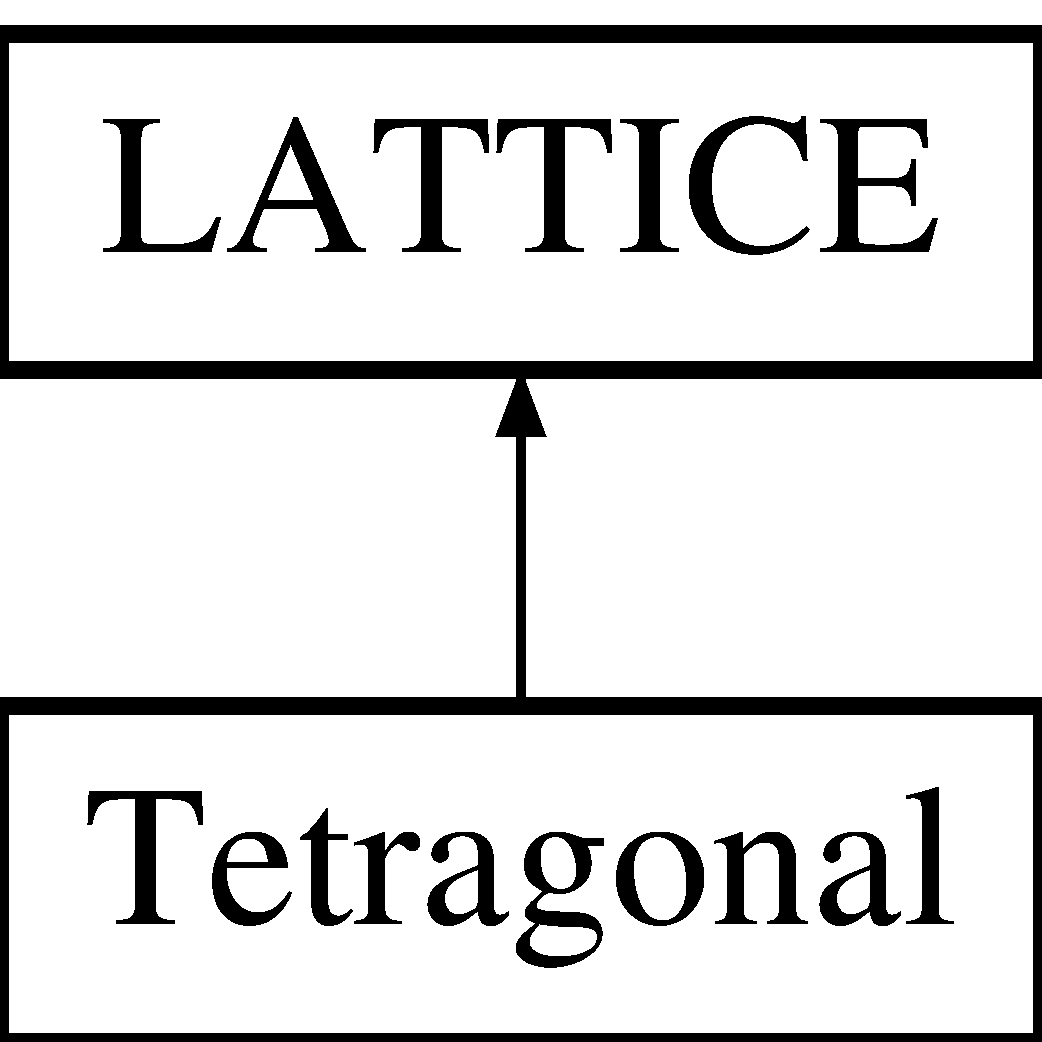
\includegraphics[height=2.000000cm]{class_tetragonal}
\end{center}
\end{figure}
\subsection*{Public Member Functions}
\begin{DoxyCompactItemize}
\item 
\hyperlink{class_tetragonal_af2a4fecb021d66c6f208329e673408d0}{Tetragonal} (double i\+\_\+alat, double i\+\_\+clat, char i\+\_\+lstyle\mbox{[}$\,$\mbox{]}, char $\ast$i\+\_\+element)
\item 
\hyperlink{class_tetragonal_a37c3ca8df43e27431f8e50b2f9860d7e}{$\sim$\+Tetragonal} ()
\end{DoxyCompactItemize}
\subsection*{Private Member Functions}
\begin{DoxyCompactItemize}
\item 
void \hyperlink{class_tetragonal_af3dfd15199eb890e8191fdf37f45bf19}{primitive} ()
\item 
void \hyperlink{class_tetragonal_a1d5a55a84ae34d7fc565d050eafdd5c6}{B\+C\+C} ()
\item 
void \hyperlink{class_tetragonal_a1a795789398fdc7ede8c0a997c72abd0}{F\+C\+C} ()
\end{DoxyCompactItemize}
\subsection*{Additional Inherited Members}


\subsection{Constructor \& Destructor Documentation}
\hypertarget{class_tetragonal_af2a4fecb021d66c6f208329e673408d0}{}\index{Tetragonal@{Tetragonal}!Tetragonal@{Tetragonal}}
\index{Tetragonal@{Tetragonal}!Tetragonal@{Tetragonal}}
\subsubsection[{Tetragonal}]{\setlength{\rightskip}{0pt plus 5cm}Tetragonal\+::\+Tetragonal (
\begin{DoxyParamCaption}
\item[{double}]{i\+\_\+alat, }
\item[{double}]{i\+\_\+clat, }
\item[{char}]{i\+\_\+lstyle\mbox{[}$\,$\mbox{]}, }
\item[{char $\ast$}]{i\+\_\+element}
\end{DoxyParamCaption}
)}\label{class_tetragonal_af2a4fecb021d66c6f208329e673408d0}
\hypertarget{class_tetragonal_a37c3ca8df43e27431f8e50b2f9860d7e}{}\index{Tetragonal@{Tetragonal}!````~Tetragonal@{$\sim$\+Tetragonal}}
\index{````~Tetragonal@{$\sim$\+Tetragonal}!Tetragonal@{Tetragonal}}
\subsubsection[{$\sim$\+Tetragonal}]{\setlength{\rightskip}{0pt plus 5cm}Tetragonal\+::$\sim$\+Tetragonal (
\begin{DoxyParamCaption}
{}
\end{DoxyParamCaption}
)}\label{class_tetragonal_a37c3ca8df43e27431f8e50b2f9860d7e}


\subsection{Member Function Documentation}
\hypertarget{class_tetragonal_a1d5a55a84ae34d7fc565d050eafdd5c6}{}\index{Tetragonal@{Tetragonal}!B\+C\+C@{B\+C\+C}}
\index{B\+C\+C@{B\+C\+C}!Tetragonal@{Tetragonal}}
\subsubsection[{B\+C\+C}]{\setlength{\rightskip}{0pt plus 5cm}void Tetragonal\+::\+B\+C\+C (
\begin{DoxyParamCaption}
{}
\end{DoxyParamCaption}
)\hspace{0.3cm}{\ttfamily [private]}}\label{class_tetragonal_a1d5a55a84ae34d7fc565d050eafdd5c6}
\hypertarget{class_tetragonal_a1a795789398fdc7ede8c0a997c72abd0}{}\index{Tetragonal@{Tetragonal}!F\+C\+C@{F\+C\+C}}
\index{F\+C\+C@{F\+C\+C}!Tetragonal@{Tetragonal}}
\subsubsection[{F\+C\+C}]{\setlength{\rightskip}{0pt plus 5cm}void Tetragonal\+::\+F\+C\+C (
\begin{DoxyParamCaption}
{}
\end{DoxyParamCaption}
)\hspace{0.3cm}{\ttfamily [private]}}\label{class_tetragonal_a1a795789398fdc7ede8c0a997c72abd0}
\hypertarget{class_tetragonal_af3dfd15199eb890e8191fdf37f45bf19}{}\index{Tetragonal@{Tetragonal}!primitive@{primitive}}
\index{primitive@{primitive}!Tetragonal@{Tetragonal}}
\subsubsection[{primitive}]{\setlength{\rightskip}{0pt plus 5cm}void Tetragonal\+::primitive (
\begin{DoxyParamCaption}
{}
\end{DoxyParamCaption}
)\hspace{0.3cm}{\ttfamily [private]}}\label{class_tetragonal_af3dfd15199eb890e8191fdf37f45bf19}


The documentation for this class was generated from the following file\+:\begin{DoxyCompactItemize}
\item 
src/structures/\hyperlink{tetragonal_8h}{tetragonal.\+h}\end{DoxyCompactItemize}

\hypertarget{class_write}{}\section{Write Class Reference}
\label{class_write}\index{Write@{Write}}


\subsection{Detailed Description}
\subsection*{{\bfseries Purpose\+:} }

\begin{DoxyVerb}/********************************************************************************\
/  Class for writing atomic crystal structure data in various DFT and MD formats \
/  Currently, this class supports the following file formats:                    \
/          MSI/DMol .car format,                                                 \
/          LAMMPS input format,                                                  \
/          VASP 5.x.x POSCAR format, Direct or Cartesian, no Selective Dynamics  \
/                                                                                \
/********************************************************************************\
\end{DoxyVerb}


\begin{DoxyAuthor}{Author}
Joseph M. Gonzalez
\end{DoxyAuthor}
\begin{DoxyVersion}{Version}
0.\+1
\end{DoxyVersion}
\begin{DoxyDate}{Date}
Sep 13, 2015 19\+:16\+:20
\end{DoxyDate}
{\bfseries Contact} ~\newline
 \href{mailto:jmgonza6@mail.usf.edu}{\tt jmgonza6@mail.\+usf.\+edu} \subsection*{Public Member Functions}
\begin{DoxyCompactItemize}
\item 
\hyperlink{class_write_ad38d186b30ba3068550a3eec7879c433}{Write} ()
\item 
\hyperlink{class_write_a229158e0f40b815df57224e32c1fa377}{$\sim$\+Write} ()
\item 
void \hyperlink{class_write_a01d6843fd3be8283ce78978b77fcf4f8}{dmol} (char outname\mbox{[}$\,$\mbox{]}, int natoms, std\+::vector$<$ double $>$ a1, std\+::vector$<$ double $>$ a2, std\+::vector$<$ double $>$ a3, \hyperlink{structatom__t}{atom\+\_\+t} $\ast$atoms, std\+::vector$<$ std\+::string $>$ species\+List, std\+::vector$<$ int $>$ species\+Count)
\begin{DoxyCompactList}\small\item\em \hyperlink{class_write}{Write} the crystal structure defined by the user in the D\+Mol {\ttfamily .car} format. \end{DoxyCompactList}\item 
void \hyperlink{class_write_a410edc16f935d4f9d472c1193a023d1f}{lammps} (char outname\mbox{[}$\,$\mbox{]}, char comment\mbox{[}$\,$\mbox{]}, int natoms, std\+::vector$<$ double $>$ a1, std\+::vector$<$ double $>$ a2, std\+::vector$<$ double $>$ a3, \hyperlink{structatom__t}{atom\+\_\+t} $\ast$atoms, std\+::vector$<$ std\+::string $>$ species\+List)
\begin{DoxyCompactList}\small\item\em \hyperlink{class_write}{Write} the crystal structure defined by the user in the L\+A\+M\+M\+P\+S {\ttfamily .input} format. \end{DoxyCompactList}\item 
void \hyperlink{class_write_a22efe8e3dbca6d3e85488a6c7952903c}{poscar} (char comment\mbox{[}$\,$\mbox{]}, int natoms, std\+::vector$<$ double $>$ a1, std\+::vector$<$ double $>$ a2, std\+::vector$<$ double $>$ a3, \hyperlink{structatom__t}{atom\+\_\+t} $\ast$atoms, int fractional, std\+::vector$<$ std\+::string $>$ species\+List, std\+::vector$<$ int $>$ species\+Count)
\begin{DoxyCompactList}\small\item\em \hyperlink{class_write}{Write} the crystal structure defined by the user in the V\+A\+S\+P {\ttfamily P\+O\+S\+C\+A\+R} format. \end{DoxyCompactList}\end{DoxyCompactItemize}
\subsection*{Private Member Functions}
\begin{DoxyCompactItemize}
\item 
std\+::string \hyperlink{class_write_ae9c6a2ab3e82a7462bc1c273bbf41e5e}{mass2elem} (double mass)
\item 
double \hyperlink{class_write_a7fbec7da3629cb3441660afa490c3ef6}{elem2mass} (std\+::string element)
\end{DoxyCompactItemize}
\subsection*{Private Attributes}
\begin{DoxyCompactItemize}
\item 
\hyperlink{class_memory}{Memory} $\ast$ \hyperlink{class_write_ac6d11e0db370053dda204d7de9f6a605}{memory}
\end{DoxyCompactItemize}


\subsection{Constructor \& Destructor Documentation}
\hypertarget{class_write_ad38d186b30ba3068550a3eec7879c433}{}\index{Write@{Write}!Write@{Write}}
\index{Write@{Write}!Write@{Write}}
\subsubsection[{Write}]{\setlength{\rightskip}{0pt plus 5cm}Write\+::\+Write (
\begin{DoxyParamCaption}
{}
\end{DoxyParamCaption}
)}\label{class_write_ad38d186b30ba3068550a3eec7879c433}
\hypertarget{class_write_a229158e0f40b815df57224e32c1fa377}{}\index{Write@{Write}!````~Write@{$\sim$\+Write}}
\index{````~Write@{$\sim$\+Write}!Write@{Write}}
\subsubsection[{$\sim$\+Write}]{\setlength{\rightskip}{0pt plus 5cm}Write\+::$\sim$\+Write (
\begin{DoxyParamCaption}
{}
\end{DoxyParamCaption}
)}\label{class_write_a229158e0f40b815df57224e32c1fa377}


\subsection{Member Function Documentation}
\hypertarget{class_write_a01d6843fd3be8283ce78978b77fcf4f8}{}\index{Write@{Write}!dmol@{dmol}}
\index{dmol@{dmol}!Write@{Write}}
\subsubsection[{dmol}]{\setlength{\rightskip}{0pt plus 5cm}void Write\+::dmol (
\begin{DoxyParamCaption}
\item[{char}]{outname\mbox{[}$\,$\mbox{]}, }
\item[{int}]{natoms, }
\item[{std\+::vector$<$ double $>$}]{a1, }
\item[{std\+::vector$<$ double $>$}]{a2, }
\item[{std\+::vector$<$ double $>$}]{a3, }
\item[{{\bf atom\+\_\+t} $\ast$}]{atoms, }
\item[{std\+::vector$<$ std\+::string $>$}]{species\+List, }
\item[{std\+::vector$<$ int $>$}]{species\+Count}
\end{DoxyParamCaption}
)}\label{class_write_a01d6843fd3be8283ce78978b77fcf4f8}


\hyperlink{class_write}{Write} the crystal structure defined by the user in the D\+Mol {\ttfamily .car} format. 


\begin{DoxyParams}[1]{Parameters}
\mbox{\tt in}  & {\em outname} & -\/ name of the regular file for writing \\
\hline
\mbox{\tt in}  & {\em natoms} & -\/ total number of atoms created \\
\hline
\mbox{\tt in}  & {\em a1} & -\/ major lattice vector along x \\
\hline
\mbox{\tt in}  & {\em a2} & -\/ lattice vector in xy plane \\
\hline
\mbox{\tt in}  & {\em a3} & -\/ lattice vector in xyz plane \\
\hline
\mbox{\tt in}  & {\em atoms} & -\/ Structure containing the atomic positions, and atomic type numbers \\
\hline
\mbox{\tt in}  & {\em species\+List} & -\/ list of all unique elements \\
\hline
\mbox{\tt in}  & {\em species\+Count} & -\/ 1\+D vector containing the count of each type in {\ttfamily species\+List} \\
\hline
\end{DoxyParams}
\hypertarget{class_write_a7fbec7da3629cb3441660afa490c3ef6}{}\index{Write@{Write}!elem2mass@{elem2mass}}
\index{elem2mass@{elem2mass}!Write@{Write}}
\subsubsection[{elem2mass}]{\setlength{\rightskip}{0pt plus 5cm}double Write\+::elem2mass (
\begin{DoxyParamCaption}
\item[{std\+::string}]{element}
\end{DoxyParamCaption}
)\hspace{0.3cm}{\ttfamily [private]}}\label{class_write_a7fbec7da3629cb3441660afa490c3ef6}
\hypertarget{class_write_a410edc16f935d4f9d472c1193a023d1f}{}\index{Write@{Write}!lammps@{lammps}}
\index{lammps@{lammps}!Write@{Write}}
\subsubsection[{lammps}]{\setlength{\rightskip}{0pt plus 5cm}void Write\+::lammps (
\begin{DoxyParamCaption}
\item[{char}]{outname\mbox{[}$\,$\mbox{]}, }
\item[{char}]{comment\mbox{[}$\,$\mbox{]}, }
\item[{int}]{natoms, }
\item[{std\+::vector$<$ double $>$}]{a1, }
\item[{std\+::vector$<$ double $>$}]{a2, }
\item[{std\+::vector$<$ double $>$}]{a3, }
\item[{{\bf atom\+\_\+t} $\ast$}]{atoms, }
\item[{std\+::vector$<$ std\+::string $>$}]{species\+List}
\end{DoxyParamCaption}
)}\label{class_write_a410edc16f935d4f9d472c1193a023d1f}


\hyperlink{class_write}{Write} the crystal structure defined by the user in the L\+A\+M\+M\+P\+S {\ttfamily .input} format. 


\begin{DoxyParams}[1]{Parameters}
\mbox{\tt in}  & {\em outname} & -\/ name of the regular file for writing \\
\hline
\mbox{\tt in}  & {\em comment} & -\/ a comment line describing the crystal \\
\hline
\mbox{\tt in}  & {\em natoms} & -\/ total number of atoms created \\
\hline
\mbox{\tt in}  & {\em a1} & -\/ major lattice vector along x \\
\hline
\mbox{\tt in}  & {\em a2} & -\/ lattice vector in xy plane \\
\hline
\mbox{\tt in}  & {\em a3} & -\/ lattice vector in xyz plane \\
\hline
\mbox{\tt in}  & {\em atoms} & -\/ Structure containing the atomic positions, and atomic type numbers \\
\hline
\mbox{\tt in}  & {\em species\+List} & -\/ list of all unique element strings \\
\hline
\end{DoxyParams}
\hypertarget{class_write_ae9c6a2ab3e82a7462bc1c273bbf41e5e}{}\index{Write@{Write}!mass2elem@{mass2elem}}
\index{mass2elem@{mass2elem}!Write@{Write}}
\subsubsection[{mass2elem}]{\setlength{\rightskip}{0pt plus 5cm}std\+::string Write\+::mass2elem (
\begin{DoxyParamCaption}
\item[{double}]{mass}
\end{DoxyParamCaption}
)\hspace{0.3cm}{\ttfamily [private]}}\label{class_write_ae9c6a2ab3e82a7462bc1c273bbf41e5e}
\hypertarget{class_write_a22efe8e3dbca6d3e85488a6c7952903c}{}\index{Write@{Write}!poscar@{poscar}}
\index{poscar@{poscar}!Write@{Write}}
\subsubsection[{poscar}]{\setlength{\rightskip}{0pt plus 5cm}void Write\+::poscar (
\begin{DoxyParamCaption}
\item[{char}]{comment\mbox{[}$\,$\mbox{]}, }
\item[{int}]{natoms, }
\item[{std\+::vector$<$ double $>$}]{a1, }
\item[{std\+::vector$<$ double $>$}]{a2, }
\item[{std\+::vector$<$ double $>$}]{a3, }
\item[{{\bf atom\+\_\+t} $\ast$}]{atoms, }
\item[{int}]{fractional, }
\item[{std\+::vector$<$ std\+::string $>$}]{species\+List, }
\item[{std\+::vector$<$ int $>$}]{species\+Count}
\end{DoxyParamCaption}
)}\label{class_write_a22efe8e3dbca6d3e85488a6c7952903c}


\hyperlink{class_write}{Write} the crystal structure defined by the user in the V\+A\+S\+P {\ttfamily P\+O\+S\+C\+A\+R} format. 


\begin{DoxyParams}[1]{Parameters}
\mbox{\tt in}  & {\em comment} & -\/ a comment line describing the crystal \\
\hline
\mbox{\tt in}  & {\em natoms} & -\/ total number of atoms created \\
\hline
\mbox{\tt in}  & {\em a1} & -\/ major lattice vector along x \\
\hline
\mbox{\tt in}  & {\em a2} & -\/ lattice vector in xy plane \\
\hline
\mbox{\tt in}  & {\em a3} & -\/ lattice vector in xyz plane \\
\hline
\mbox{\tt in}  & {\em atoms} & -\/ Structure containing the atomic positions, and atomic type numbers \\
\hline
\mbox{\tt in}  & {\em fractional} & -\/ {\ttfamily coords} is in fractional units \begin{DoxyItemize}
\item {\ttfamily 1} = fractional {\ttfamily 0} = cartesian \end{DoxyItemize}
\\
\hline
\mbox{\tt in}  & {\em species\+List} & -\/ list of all unique element strings \\
\hline
\mbox{\tt in}  & {\em species\+Count} & -\/ 1\+D vector containing the count of each type in {\ttfamily species\+List} \\
\hline
\end{DoxyParams}


\subsection{Field Documentation}
\hypertarget{class_write_ac6d11e0db370053dda204d7de9f6a605}{}\index{Write@{Write}!memory@{memory}}
\index{memory@{memory}!Write@{Write}}
\subsubsection[{memory}]{\setlength{\rightskip}{0pt plus 5cm}{\bf Memory}$\ast$ Write\+::memory\hspace{0.3cm}{\ttfamily [private]}}\label{class_write_ac6d11e0db370053dda204d7de9f6a605}


The documentation for this class was generated from the following file\+:\begin{DoxyCompactItemize}
\item 
src/util/\hyperlink{write_8h}{write.\+h}\end{DoxyCompactItemize}

\chapter{File Documentation}
\hypertarget{mainpage_8dox}{}\section{mainpage.\+dox File Reference}
\label{mainpage_8dox}\index{mainpage.\+dox@{mainpage.\+dox}}

\hypertarget{gui_8h}{}\section{src/gui/gui.h File Reference}
\label{gui_8h}\index{src/gui/gui.\+h@{src/gui/gui.\+h}}
\subsection*{Data Structures}
\begin{DoxyCompactItemize}
\item 
class \hyperlink{class_gui}{Gui}
\end{DoxyCompactItemize}
\subsection*{Macros}
\begin{DoxyCompactItemize}
\item 
\#define \hyperlink{gui_8h_ace5acd139435dd7801845337ad58f753}{F\+R\+W\+I\+D\+T\+H}~600
\begin{DoxyCompactList}\small\item\em width of the frame inside each tab \end{DoxyCompactList}\item 
\#define \hyperlink{gui_8h_ac011eb0bcbc694af2b955827dbfc4b01}{F\+R\+H\+E\+I\+G\+H\+T}~400
\begin{DoxyCompactList}\small\item\em height of the frame inside each tab \end{DoxyCompactList}\end{DoxyCompactItemize}


\subsection{Macro Definition Documentation}
\hypertarget{gui_8h_ac011eb0bcbc694af2b955827dbfc4b01}{}\index{gui.\+h@{gui.\+h}!F\+R\+H\+E\+I\+G\+H\+T@{F\+R\+H\+E\+I\+G\+H\+T}}
\index{F\+R\+H\+E\+I\+G\+H\+T@{F\+R\+H\+E\+I\+G\+H\+T}!gui.\+h@{gui.\+h}}
\subsubsection[{F\+R\+H\+E\+I\+G\+H\+T}]{\setlength{\rightskip}{0pt plus 5cm}\#define F\+R\+H\+E\+I\+G\+H\+T~400}\label{gui_8h_ac011eb0bcbc694af2b955827dbfc4b01}


height of the frame inside each tab 

\hypertarget{gui_8h_ace5acd139435dd7801845337ad58f753}{}\index{gui.\+h@{gui.\+h}!F\+R\+W\+I\+D\+T\+H@{F\+R\+W\+I\+D\+T\+H}}
\index{F\+R\+W\+I\+D\+T\+H@{F\+R\+W\+I\+D\+T\+H}!gui.\+h@{gui.\+h}}
\subsubsection[{F\+R\+W\+I\+D\+T\+H}]{\setlength{\rightskip}{0pt plus 5cm}\#define F\+R\+W\+I\+D\+T\+H~600}\label{gui_8h_ace5acd139435dd7801845337ad58f753}


width of the frame inside each tab 


\hypertarget{render_8h}{}\section{src/gui/render.h File Reference}
\label{render_8h}\index{src/gui/render.\+h@{src/gui/render.\+h}}


\subsection{Detailed Description}
\subsection*{{\bfseries Purpose\+:} }

\begin{DoxyVerb}/*****************************************************************************************\
/  Simple rendering engine to display the crystal built by the user during a GUI session  \
/                                                                                         \
/  Borrowed in part from example3/5.cpp of the GLUI tutorials.                            \
/*****************************************************************************************\
\end{DoxyVerb}


\subsection*{{\bfseries User} interaction\+: }

\begin{DoxyVerb}*
*  Mouse events:
*     Left mouse            rotate, zoom
*     Right mouse           menu
*
*  Keyboard events:
*     'A'                   display atoms and unit cell
*     'a'                   display atoms only
*     'B'                   display bonds, uniform nearest neighbor cutoff
*     'b'                   hide bonds
*     'C'                   increase nearest neighbor cutoff
*     'c'                   decrease nearest neighbor cutoff
*     'e'                   exit and save the data from the rendering scene
*     'o'                   orthographic projection of the crystal
*     'p'                   perspective projection of the crystal
*     'r' then LeftButton   rotate the crystal in all 3 dimensions
*     'W'                   change background to white and bounding box to black
*     'w'                   change background to black and bounding box to white
*     'z' then LeftButton   zoom toward/away from the crystal
*     '0'                   reset orientation of crystal to looking down z toward xy plane
*     '1'                   view the xz "a-c" plane of the crystal
*     '2'                   view the yz "b-c" plane of the crystal
*     '3'                   rotate crystal about x by -45˚, and then -45˚ about z, 'psuedo' perspective view
*     '+'                   increase the particle radius uniformly
*     '-'                   decrease the particle radius uniformly
*
*     Up arrow              Shift the crystal in positive vertical screen direction
*     Down arrow            Shift the crystal in negative vertical screen direction
*     Left arrow            Shift the crystal in negative horizontal screen direction
*     Right arrow           Shift the crystal in positive horizontal screen direction
*
\end{DoxyVerb}
 \begin{DoxyAuthor}{Author}
Joseph M. Gonzalez
\end{DoxyAuthor}
\begin{DoxyVersion}{Version}
0.\+9
\end{DoxyVersion}
\begin{DoxyDate}{Date}
Sep 27, 2015 19\+:16\+:20
\end{DoxyDate}
{\bfseries Contact} ~\newline
 \href{mailto:jmgonza6@mail.usf.edu}{\tt jmgonza6@mail.\+usf.\+edu} \subsection*{Macros}
\begin{DoxyCompactItemize}
\item 
\#define \hyperlink{render_8h_ada0bcbc219bc46638a6f40092491e704}{W\+W\+I\+D\+T\+H}~600
\begin{DoxyCompactList}\small\item\em width of the rendering window \end{DoxyCompactList}\item 
\#define \hyperlink{render_8h_a2eddba14a242c88a398413c84af5c052}{W\+H\+E\+I\+G\+H\+T}~600
\begin{DoxyCompactList}\small\item\em height of the rendering window \end{DoxyCompactList}\item 
\#define \hyperlink{render_8h_a7634176dc486701cee85ef1620b0577e}{V\+P\+O\+R\+T\+\_\+\+S\+I\+Z\+E}~60
\begin{DoxyCompactList}\small\item\em size of the view port, V\+P\+O\+R\+T\+\_\+\+S\+I\+Z\+Ex\+V\+P\+O\+R\+T\+\_\+\+S\+I\+Z\+E \end{DoxyCompactList}\end{DoxyCompactItemize}
\subsection*{Enumerations}
\begin{DoxyCompactItemize}
\item 
enum \hyperlink{render_8h_adfe2f0ef8da517b3f0e87cbf0cb31b9a}{Left\+Button} \{ \hyperlink{render_8h_adfe2f0ef8da517b3f0e87cbf0cb31b9aa3dcfe0046eb5876e287dbf0914819b16}{R\+O\+T\+A\+T\+E}, 
\hyperlink{render_8h_adfe2f0ef8da517b3f0e87cbf0cb31b9aa593be05a10070b4e7e0856e20590eaaf}{S\+C\+A\+L\+E}, 
\hyperlink{render_8h_adfe2f0ef8da517b3f0e87cbf0cb31b9aabc6501410409b0638909b580970b35f7}{T\+R\+A\+N\+S\+L\+A\+T\+E}, 
\hyperlink{render_8h_adfe2f0ef8da517b3f0e87cbf0cb31b9aa52e3d57e4410a3f781e113a401378c42}{D\+R\+A\+G}
 \}
\item 
enum \{ \\*
\hyperlink{render_8h_a06fc87d81c62e9abb8790b6e5713c55ba157e8676195b7afd68bf23bb95f8a160}{S\+H\+O\+W\+A\+L\+L}, 
\hyperlink{render_8h_a06fc87d81c62e9abb8790b6e5713c55ba799f70fd8773687e236be553ca91b67e}{A\+T\+O\+M\+S\+O\+N\+L\+Y}, 
\hyperlink{render_8h_a06fc87d81c62e9abb8790b6e5713c55ba05553b32a8a8f5b56e5257e3aad9e5b2}{B\+O\+N\+D\+S}, 
\hyperlink{render_8h_a06fc87d81c62e9abb8790b6e5713c55babdf68f43541b0960e06ff2a4e2c57234}{B\+L\+A\+C\+K\+B}, 
\\*
\hyperlink{render_8h_a06fc87d81c62e9abb8790b6e5713c55ba6c28891fe95f0ea3bce909d2238b87cd}{W\+H\+I\+T\+E\+B}
 \}
\end{DoxyCompactItemize}
\subsection*{Functions}
\begin{DoxyCompactItemize}
\item 
void \hyperlink{render_8h_acc19403a720bda8d74dcad7109f33a79}{gl\+\_\+init} ()
\begin{DoxyCompactList}\small\item\em Initialize the Open G\+L and G\+L\+U\+T infrastructure with window size, lighting, positions, etc. \end{DoxyCompactList}\item 
void \hyperlink{render_8h_aa698526fd08a0e1dd5a53d86e38a735f}{gl\+\_\+menu\+\_\+init} ()
\begin{DoxyCompactList}\small\item\em Initialize the right mouse button menu with scene display options. \end{DoxyCompactList}\item 
int \hyperlink{render_8h_a4cf3ecdb7a4952d258bbabf29ad7fcef}{build\+\_\+nn\+\_\+list} ()
\begin{DoxyCompactList}\small\item\em Construct a nearest neighbor list for each particle, naive n$^\wedge$2 algorithm. \end{DoxyCompactList}\item 
int \hyperlink{render_8h_a603668b9400ce52fcc5592b076726956}{render\+\_\+init} (int natom, std\+::vector$<$ double $>$ a1, std\+::vector$<$ double $>$ a2, std\+::vector$<$ double $>$ a3, \hyperlink{structatom__t}{atom\+\_\+t} $\ast$atoms\+In, std\+::vector$<$ std\+::string $>$ species, std\+::vector$<$ int $>$ elem\+Count)
\begin{DoxyCompactList}\small\item\em Locally store the data entered by the user during the gui session. \end{DoxyCompactList}\item 
int \hyperlink{render_8h_afe311122da1ef07a93e881d080fde16d}{init\+\_\+call\+\_\+lists} (int list)
\begin{DoxyCompactList}\small\item\em Selectively initialize the atomic and or unit cell data from a G\+U\+I session Draws the objects and stores the data in a gl\+List. These lists make rendering ~\newline
much more efficient with a simple call to gl\+Call\+List() \end{DoxyCompactList}\item 
void \hyperlink{render_8h_a42d4ed068625dac47e760c48ef25271f}{init\+\_\+axes\+\_\+list} ()
\begin{DoxyCompactList}\small\item\em Initialize the coordinate axes for the scene~\newline
x = red , y = green, blue = z~\newline
Drawn using G\+L\+\_\+\+L\+I\+N\+E\+\_\+\+S\+T\+R\+I\+P and stores the data in a gl\+List, {\ttfamily Axes\+List}. \end{DoxyCompactList}\item 
void \hyperlink{render_8h_ad3c2cf92be0e0ba02444723d497b89b1}{init\+\_\+bbox\+\_\+list} ()
\begin{DoxyCompactList}\small\item\em Initialize the periodic unit cell~\newline
Drawn using G\+L\+\_\+\+L\+I\+N\+E\+\_\+\+S\+T\+R\+I\+P and stores the data in a gl\+List, {\ttfamily Unit\+Cell\+List}. \end{DoxyCompactList}\item 
void \hyperlink{render_8h_ac2fad95aa2bfbc751e262c7019122c4a}{init\+\_\+atoms\+\_\+list} ()
\begin{DoxyCompactList}\small\item\em Initialize the atomic coordinates~\newline
 The particles are drawn as glu\+Solid\+Sphere() objects and stores ~\newline
 the data in a gl\+List, {\ttfamily Atoms\+List}. \end{DoxyCompactList}\item 
void \hyperlink{render_8h_affc94ce23a038bcb6aa0f65c8d3d81d7}{show\+\_\+all} (int vport)
\begin{DoxyCompactList}\small\item\em Render unit cell, cartesian axes, and atoms in all 4 view ports. \end{DoxyCompactList}\item 
void \hyperlink{render_8h_ae8603f8aa531cc92d8c7eb92314df104}{atoms\+\_\+only} (int vport)
\begin{DoxyCompactList}\small\item\em Render atoms only in {\ttfamily vport} \end{DoxyCompactList}\item 
void \hyperlink{render_8h_a73b6df8ac67794cf1ad91f18c71c4a87}{reshape\+\_\+window} (int width, int height)
\begin{DoxyCompactList}\small\item\em Reshape the window. \end{DoxyCompactList}\item 
void \hyperlink{render_8h_a82ac60a8b106733190548d2addae5fed}{set\+\_\+display\+\_\+type} (int value)
\begin{DoxyCompactList}\small\item\em Set the display type. \end{DoxyCompactList}\item 
void \hyperlink{render_8h_a59c3084a0fed1d65a1fb9dbba6c3e56e}{kill\+\_\+main\+\_\+window} (int value)
\begin{DoxyCompactList}\small\item\em Activate/kill main rendering window. \end{DoxyCompactList}\item 
void \hyperlink{render_8h_adf73420516ee08d031f36d51cc78ee35}{render\+\_\+data} ()
\begin{DoxyCompactList}\small\item\em Set the display type, the projection type, initialize call lists, and handle scene modifications~\newline
 Called by {\ttfamily glut\+Display\+Func()}. \end{DoxyCompactList}\item 
void \hyperlink{render_8h_acdabd89f3b25ddf7ea434ed8d48984f2}{draw\+\_\+nn\+\_\+bond} (float x1, float y1, float z1, float x2, float y2, float z2, float radius, int stacks)
\begin{DoxyCompactList}\small\item\em Draw a solid cylinder between nearest neighbors. \end{DoxyCompactList}\item 
void \hyperlink{render_8h_a4f4a5ee87047e3597dd1e8215aa75a8e}{keyboard\+\_\+event} (unsigned char ch, int x, int y)
\begin{DoxyCompactList}\small\item\em Track and process keyboard signals. \end{DoxyCompactList}\item 
void \hyperlink{render_8h_ac0a35b8a6660e9a351626495193ba3ec}{mouse\+\_\+clicked} (int button, int state, int x, int y)
\begin{DoxyCompactList}\small\item\em Track and process mouse signals. \end{DoxyCompactList}\item 
void \hyperlink{render_8h_afbef1733d1ecc6ccb52399b5c8ef749a}{mouse\+\_\+moved} (int x, int y)
\begin{DoxyCompactList}\small\item\em Track and process orientation of viewports from mouse/motion events. \end{DoxyCompactList}\item 
void \hyperlink{render_8h_aefc88e0fd48154a58790e21c750e269c}{special\+\_\+key\+\_\+pressed} (int key, int xx, int yy)
\begin{DoxyCompactList}\small\item\em Track and process special keyboard signals, arrows, alt, ctrl, etc. being pressed. \end{DoxyCompactList}\item 
void \hyperlink{render_8h_ae15071ba4a0f9e84d7612e05d0ec7fc3}{special\+\_\+key\+\_\+release} (int key, int x, int y)
\begin{DoxyCompactList}\small\item\em Track and process special keyboard signals, arrows, alt, ctrl, etc. being released. \end{DoxyCompactList}\item 
void \hyperlink{render_8h_a9d27ea12940f31238fc1105f5e79be80}{Get\+O\+G\+L\+Pos} (int x, int y)
\item 
void \hyperlink{render_8h_a781f6a13ca1a09f7d817caff7f763fb0}{build\+\_\+color\+Table} ()
\begin{DoxyCompactList}\small\item\em Load an array with rgb values for coloring different atomic species.~\newline
The coloring scheme used is C\+P\+K, which is the same as in Jmol. \end{DoxyCompactList}\end{DoxyCompactItemize}


\subsection{Macro Definition Documentation}
\hypertarget{render_8h_a7634176dc486701cee85ef1620b0577e}{}\index{render.\+h@{render.\+h}!V\+P\+O\+R\+T\+\_\+\+S\+I\+Z\+E@{V\+P\+O\+R\+T\+\_\+\+S\+I\+Z\+E}}
\index{V\+P\+O\+R\+T\+\_\+\+S\+I\+Z\+E@{V\+P\+O\+R\+T\+\_\+\+S\+I\+Z\+E}!render.\+h@{render.\+h}}
\subsubsection[{V\+P\+O\+R\+T\+\_\+\+S\+I\+Z\+E}]{\setlength{\rightskip}{0pt plus 5cm}\#define V\+P\+O\+R\+T\+\_\+\+S\+I\+Z\+E~60}\label{render_8h_a7634176dc486701cee85ef1620b0577e}


size of the view port, V\+P\+O\+R\+T\+\_\+\+S\+I\+Z\+Ex\+V\+P\+O\+R\+T\+\_\+\+S\+I\+Z\+E 

\hypertarget{render_8h_a2eddba14a242c88a398413c84af5c052}{}\index{render.\+h@{render.\+h}!W\+H\+E\+I\+G\+H\+T@{W\+H\+E\+I\+G\+H\+T}}
\index{W\+H\+E\+I\+G\+H\+T@{W\+H\+E\+I\+G\+H\+T}!render.\+h@{render.\+h}}
\subsubsection[{W\+H\+E\+I\+G\+H\+T}]{\setlength{\rightskip}{0pt plus 5cm}\#define W\+H\+E\+I\+G\+H\+T~600}\label{render_8h_a2eddba14a242c88a398413c84af5c052}


height of the rendering window 

\hypertarget{render_8h_ada0bcbc219bc46638a6f40092491e704}{}\index{render.\+h@{render.\+h}!W\+W\+I\+D\+T\+H@{W\+W\+I\+D\+T\+H}}
\index{W\+W\+I\+D\+T\+H@{W\+W\+I\+D\+T\+H}!render.\+h@{render.\+h}}
\subsubsection[{W\+W\+I\+D\+T\+H}]{\setlength{\rightskip}{0pt plus 5cm}\#define W\+W\+I\+D\+T\+H~600}\label{render_8h_ada0bcbc219bc46638a6f40092491e704}


width of the rendering window 



\subsection{Enumeration Type Documentation}
\hypertarget{render_8h_a06fc87d81c62e9abb8790b6e5713c55b}{}\subsubsection[{anonymous enum}]{\setlength{\rightskip}{0pt plus 5cm}anonymous enum}\label{render_8h_a06fc87d81c62e9abb8790b6e5713c55b}
\begin{Desc}
\item[Enumerator]\par
\begin{description}
\index{S\+H\+O\+W\+A\+L\+L@{S\+H\+O\+W\+A\+L\+L}!render.\+h@{render.\+h}}\index{render.\+h@{render.\+h}!S\+H\+O\+W\+A\+L\+L@{S\+H\+O\+W\+A\+L\+L}}\item[{\em 
\hypertarget{render_8h_a06fc87d81c62e9abb8790b6e5713c55ba157e8676195b7afd68bf23bb95f8a160}{}S\+H\+O\+W\+A\+L\+L\label{render_8h_a06fc87d81c62e9abb8790b6e5713c55ba157e8676195b7afd68bf23bb95f8a160}
}]\index{A\+T\+O\+M\+S\+O\+N\+L\+Y@{A\+T\+O\+M\+S\+O\+N\+L\+Y}!render.\+h@{render.\+h}}\index{render.\+h@{render.\+h}!A\+T\+O\+M\+S\+O\+N\+L\+Y@{A\+T\+O\+M\+S\+O\+N\+L\+Y}}\item[{\em 
\hypertarget{render_8h_a06fc87d81c62e9abb8790b6e5713c55ba799f70fd8773687e236be553ca91b67e}{}A\+T\+O\+M\+S\+O\+N\+L\+Y\label{render_8h_a06fc87d81c62e9abb8790b6e5713c55ba799f70fd8773687e236be553ca91b67e}
}]\index{B\+O\+N\+D\+S@{B\+O\+N\+D\+S}!render.\+h@{render.\+h}}\index{render.\+h@{render.\+h}!B\+O\+N\+D\+S@{B\+O\+N\+D\+S}}\item[{\em 
\hypertarget{render_8h_a06fc87d81c62e9abb8790b6e5713c55ba05553b32a8a8f5b56e5257e3aad9e5b2}{}B\+O\+N\+D\+S\label{render_8h_a06fc87d81c62e9abb8790b6e5713c55ba05553b32a8a8f5b56e5257e3aad9e5b2}
}]\index{B\+L\+A\+C\+K\+B@{B\+L\+A\+C\+K\+B}!render.\+h@{render.\+h}}\index{render.\+h@{render.\+h}!B\+L\+A\+C\+K\+B@{B\+L\+A\+C\+K\+B}}\item[{\em 
\hypertarget{render_8h_a06fc87d81c62e9abb8790b6e5713c55babdf68f43541b0960e06ff2a4e2c57234}{}B\+L\+A\+C\+K\+B\label{render_8h_a06fc87d81c62e9abb8790b6e5713c55babdf68f43541b0960e06ff2a4e2c57234}
}]\index{W\+H\+I\+T\+E\+B@{W\+H\+I\+T\+E\+B}!render.\+h@{render.\+h}}\index{render.\+h@{render.\+h}!W\+H\+I\+T\+E\+B@{W\+H\+I\+T\+E\+B}}\item[{\em 
\hypertarget{render_8h_a06fc87d81c62e9abb8790b6e5713c55ba6c28891fe95f0ea3bce909d2238b87cd}{}W\+H\+I\+T\+E\+B\label{render_8h_a06fc87d81c62e9abb8790b6e5713c55ba6c28891fe95f0ea3bce909d2238b87cd}
}]\end{description}
\end{Desc}
\hypertarget{render_8h_adfe2f0ef8da517b3f0e87cbf0cb31b9a}{}\index{render.\+h@{render.\+h}!Left\+Button@{Left\+Button}}
\index{Left\+Button@{Left\+Button}!render.\+h@{render.\+h}}
\subsubsection[{Left\+Button}]{\setlength{\rightskip}{0pt plus 5cm}enum {\bf Left\+Button}}\label{render_8h_adfe2f0ef8da517b3f0e87cbf0cb31b9a}
\begin{Desc}
\item[Enumerator]\par
\begin{description}
\index{R\+O\+T\+A\+T\+E@{R\+O\+T\+A\+T\+E}!render.\+h@{render.\+h}}\index{render.\+h@{render.\+h}!R\+O\+T\+A\+T\+E@{R\+O\+T\+A\+T\+E}}\item[{\em 
\hypertarget{render_8h_adfe2f0ef8da517b3f0e87cbf0cb31b9aa3dcfe0046eb5876e287dbf0914819b16}{}R\+O\+T\+A\+T\+E\label{render_8h_adfe2f0ef8da517b3f0e87cbf0cb31b9aa3dcfe0046eb5876e287dbf0914819b16}
}]\index{S\+C\+A\+L\+E@{S\+C\+A\+L\+E}!render.\+h@{render.\+h}}\index{render.\+h@{render.\+h}!S\+C\+A\+L\+E@{S\+C\+A\+L\+E}}\item[{\em 
\hypertarget{render_8h_adfe2f0ef8da517b3f0e87cbf0cb31b9aa593be05a10070b4e7e0856e20590eaaf}{}S\+C\+A\+L\+E\label{render_8h_adfe2f0ef8da517b3f0e87cbf0cb31b9aa593be05a10070b4e7e0856e20590eaaf}
}]\index{T\+R\+A\+N\+S\+L\+A\+T\+E@{T\+R\+A\+N\+S\+L\+A\+T\+E}!render.\+h@{render.\+h}}\index{render.\+h@{render.\+h}!T\+R\+A\+N\+S\+L\+A\+T\+E@{T\+R\+A\+N\+S\+L\+A\+T\+E}}\item[{\em 
\hypertarget{render_8h_adfe2f0ef8da517b3f0e87cbf0cb31b9aabc6501410409b0638909b580970b35f7}{}T\+R\+A\+N\+S\+L\+A\+T\+E\label{render_8h_adfe2f0ef8da517b3f0e87cbf0cb31b9aabc6501410409b0638909b580970b35f7}
}]\index{D\+R\+A\+G@{D\+R\+A\+G}!render.\+h@{render.\+h}}\index{render.\+h@{render.\+h}!D\+R\+A\+G@{D\+R\+A\+G}}\item[{\em 
\hypertarget{render_8h_adfe2f0ef8da517b3f0e87cbf0cb31b9aa52e3d57e4410a3f781e113a401378c42}{}D\+R\+A\+G\label{render_8h_adfe2f0ef8da517b3f0e87cbf0cb31b9aa52e3d57e4410a3f781e113a401378c42}
}]\end{description}
\end{Desc}


\subsection{Function Documentation}
\hypertarget{render_8h_ae8603f8aa531cc92d8c7eb92314df104}{}\index{render.\+h@{render.\+h}!atoms\+\_\+only@{atoms\+\_\+only}}
\index{atoms\+\_\+only@{atoms\+\_\+only}!render.\+h@{render.\+h}}
\subsubsection[{atoms\+\_\+only}]{\setlength{\rightskip}{0pt plus 5cm}void atoms\+\_\+only (
\begin{DoxyParamCaption}
\item[{int}]{vport}
\end{DoxyParamCaption}
)}\label{render_8h_ae8603f8aa531cc92d8c7eb92314df104}


Render atoms only in {\ttfamily vport} 


\begin{DoxyParams}[1]{Parameters}
\mbox{\tt in}  & {\em vport} & -\/ in which view port to draw \\
\hline
\end{DoxyParams}
\hypertarget{render_8h_a781f6a13ca1a09f7d817caff7f763fb0}{}\index{render.\+h@{render.\+h}!build\+\_\+color\+Table@{build\+\_\+color\+Table}}
\index{build\+\_\+color\+Table@{build\+\_\+color\+Table}!render.\+h@{render.\+h}}
\subsubsection[{build\+\_\+color\+Table}]{\setlength{\rightskip}{0pt plus 5cm}void build\+\_\+color\+Table (
\begin{DoxyParamCaption}
{}
\end{DoxyParamCaption}
)}\label{render_8h_a781f6a13ca1a09f7d817caff7f763fb0}


Load an array with rgb values for coloring different atomic species.~\newline
The coloring scheme used is C\+P\+K, which is the same as in Jmol. 

\hypertarget{render_8h_a4cf3ecdb7a4952d258bbabf29ad7fcef}{}\index{render.\+h@{render.\+h}!build\+\_\+nn\+\_\+list@{build\+\_\+nn\+\_\+list}}
\index{build\+\_\+nn\+\_\+list@{build\+\_\+nn\+\_\+list}!render.\+h@{render.\+h}}
\subsubsection[{build\+\_\+nn\+\_\+list}]{\setlength{\rightskip}{0pt plus 5cm}int build\+\_\+nn\+\_\+list (
\begin{DoxyParamCaption}
{}
\end{DoxyParamCaption}
)}\label{render_8h_a4cf3ecdb7a4952d258bbabf29ad7fcef}


Construct a nearest neighbor list for each particle, naive n$^\wedge$2 algorithm. 

\begin{DoxyReturn}{Returns}
{\ttfamily 1} if successful, {\ttfamily 0} otherwise 
\end{DoxyReturn}
\hypertarget{render_8h_acdabd89f3b25ddf7ea434ed8d48984f2}{}\index{render.\+h@{render.\+h}!draw\+\_\+nn\+\_\+bond@{draw\+\_\+nn\+\_\+bond}}
\index{draw\+\_\+nn\+\_\+bond@{draw\+\_\+nn\+\_\+bond}!render.\+h@{render.\+h}}
\subsubsection[{draw\+\_\+nn\+\_\+bond}]{\setlength{\rightskip}{0pt plus 5cm}void draw\+\_\+nn\+\_\+bond (
\begin{DoxyParamCaption}
\item[{float}]{x1, }
\item[{float}]{y1, }
\item[{float}]{z1, }
\item[{float}]{x2, }
\item[{float}]{y2, }
\item[{float}]{z2, }
\item[{float}]{radius, }
\item[{int}]{stacks}
\end{DoxyParamCaption}
)}\label{render_8h_acdabd89f3b25ddf7ea434ed8d48984f2}


Draw a solid cylinder between nearest neighbors. 


\begin{DoxyParams}[1]{Parameters}
\mbox{\tt in}  & {\em x1} & -\/ starting {\ttfamily x} coordinate of bond \\
\hline
\mbox{\tt in}  & {\em y1} & -\/ starting {\ttfamily y} coordinate of bond \\
\hline
\mbox{\tt in}  & {\em z1} & -\/ starting {\ttfamily z} coordinate of bond \\
\hline
\mbox{\tt in}  & {\em x2} & -\/ ending {\ttfamily x} coordinate of bond \\
\hline
\mbox{\tt in}  & {\em y2} & -\/ ending {\ttfamily y} coordinate of bond \\
\hline
\mbox{\tt in}  & {\em z2} & -\/ ending {\ttfamily z} coordinate of bond \\
\hline
\mbox{\tt in}  & {\em radius} & -\/ bond radius, == partilce radius / 3. \\
\hline
\mbox{\tt in}  & {\em stacks} & -\/ stacks to fill in the cylinder \\
\hline
\end{DoxyParams}
\hypertarget{render_8h_a9d27ea12940f31238fc1105f5e79be80}{}\index{render.\+h@{render.\+h}!Get\+O\+G\+L\+Pos@{Get\+O\+G\+L\+Pos}}
\index{Get\+O\+G\+L\+Pos@{Get\+O\+G\+L\+Pos}!render.\+h@{render.\+h}}
\subsubsection[{Get\+O\+G\+L\+Pos}]{\setlength{\rightskip}{0pt plus 5cm}void Get\+O\+G\+L\+Pos (
\begin{DoxyParamCaption}
\item[{int}]{x, }
\item[{int}]{y}
\end{DoxyParamCaption}
)}\label{render_8h_a9d27ea12940f31238fc1105f5e79be80}
\hypertarget{render_8h_acc19403a720bda8d74dcad7109f33a79}{}\index{render.\+h@{render.\+h}!gl\+\_\+init@{gl\+\_\+init}}
\index{gl\+\_\+init@{gl\+\_\+init}!render.\+h@{render.\+h}}
\subsubsection[{gl\+\_\+init}]{\setlength{\rightskip}{0pt plus 5cm}void gl\+\_\+init (
\begin{DoxyParamCaption}
{}
\end{DoxyParamCaption}
)}\label{render_8h_acc19403a720bda8d74dcad7109f33a79}


Initialize the Open G\+L and G\+L\+U\+T infrastructure with window size, lighting, positions, etc. 

\hypertarget{render_8h_aa698526fd08a0e1dd5a53d86e38a735f}{}\index{render.\+h@{render.\+h}!gl\+\_\+menu\+\_\+init@{gl\+\_\+menu\+\_\+init}}
\index{gl\+\_\+menu\+\_\+init@{gl\+\_\+menu\+\_\+init}!render.\+h@{render.\+h}}
\subsubsection[{gl\+\_\+menu\+\_\+init}]{\setlength{\rightskip}{0pt plus 5cm}void gl\+\_\+menu\+\_\+init (
\begin{DoxyParamCaption}
{}
\end{DoxyParamCaption}
)}\label{render_8h_aa698526fd08a0e1dd5a53d86e38a735f}


Initialize the right mouse button menu with scene display options. 

\hypertarget{render_8h_ac2fad95aa2bfbc751e262c7019122c4a}{}\index{render.\+h@{render.\+h}!init\+\_\+atoms\+\_\+list@{init\+\_\+atoms\+\_\+list}}
\index{init\+\_\+atoms\+\_\+list@{init\+\_\+atoms\+\_\+list}!render.\+h@{render.\+h}}
\subsubsection[{init\+\_\+atoms\+\_\+list}]{\setlength{\rightskip}{0pt plus 5cm}void init\+\_\+atoms\+\_\+list (
\begin{DoxyParamCaption}
{}
\end{DoxyParamCaption}
)}\label{render_8h_ac2fad95aa2bfbc751e262c7019122c4a}


Initialize the atomic coordinates~\newline
 The particles are drawn as glu\+Solid\+Sphere() objects and stores ~\newline
 the data in a gl\+List, {\ttfamily Atoms\+List}. 

\hypertarget{render_8h_a42d4ed068625dac47e760c48ef25271f}{}\index{render.\+h@{render.\+h}!init\+\_\+axes\+\_\+list@{init\+\_\+axes\+\_\+list}}
\index{init\+\_\+axes\+\_\+list@{init\+\_\+axes\+\_\+list}!render.\+h@{render.\+h}}
\subsubsection[{init\+\_\+axes\+\_\+list}]{\setlength{\rightskip}{0pt plus 5cm}void init\+\_\+axes\+\_\+list (
\begin{DoxyParamCaption}
{}
\end{DoxyParamCaption}
)}\label{render_8h_a42d4ed068625dac47e760c48ef25271f}


Initialize the coordinate axes for the scene~\newline
x = red , y = green, blue = z~\newline
Drawn using G\+L\+\_\+\+L\+I\+N\+E\+\_\+\+S\+T\+R\+I\+P and stores the data in a gl\+List, {\ttfamily Axes\+List}. 

\hypertarget{render_8h_ad3c2cf92be0e0ba02444723d497b89b1}{}\index{render.\+h@{render.\+h}!init\+\_\+bbox\+\_\+list@{init\+\_\+bbox\+\_\+list}}
\index{init\+\_\+bbox\+\_\+list@{init\+\_\+bbox\+\_\+list}!render.\+h@{render.\+h}}
\subsubsection[{init\+\_\+bbox\+\_\+list}]{\setlength{\rightskip}{0pt plus 5cm}void init\+\_\+bbox\+\_\+list (
\begin{DoxyParamCaption}
{}
\end{DoxyParamCaption}
)}\label{render_8h_ad3c2cf92be0e0ba02444723d497b89b1}


Initialize the periodic unit cell~\newline
Drawn using G\+L\+\_\+\+L\+I\+N\+E\+\_\+\+S\+T\+R\+I\+P and stores the data in a gl\+List, {\ttfamily Unit\+Cell\+List}. 

\hypertarget{render_8h_afe311122da1ef07a93e881d080fde16d}{}\index{render.\+h@{render.\+h}!init\+\_\+call\+\_\+lists@{init\+\_\+call\+\_\+lists}}
\index{init\+\_\+call\+\_\+lists@{init\+\_\+call\+\_\+lists}!render.\+h@{render.\+h}}
\subsubsection[{init\+\_\+call\+\_\+lists}]{\setlength{\rightskip}{0pt plus 5cm}int init\+\_\+call\+\_\+lists (
\begin{DoxyParamCaption}
\item[{int}]{list}
\end{DoxyParamCaption}
)}\label{render_8h_afe311122da1ef07a93e881d080fde16d}


Selectively initialize the atomic and or unit cell data from a G\+U\+I session Draws the objects and stores the data in a gl\+List. These lists make rendering ~\newline
much more efficient with a simple call to gl\+Call\+List() 


\begin{DoxyParams}[1]{Parameters}
\mbox{\tt in}  & {\em list} & -\/ which list the re-\/create \begin{DoxyItemize}
\item 1, bounding box only \item 2, coordinate axes only \item 3, atomic coordinates only \item 4, everything \end{DoxyItemize}
\\
\hline
\end{DoxyParams}
\begin{DoxyReturn}{Returns}
{\bfseries 1} if successful {\bfseries 0} otherwise 
\end{DoxyReturn}
\hypertarget{render_8h_a4f4a5ee87047e3597dd1e8215aa75a8e}{}\index{render.\+h@{render.\+h}!keyboard\+\_\+event@{keyboard\+\_\+event}}
\index{keyboard\+\_\+event@{keyboard\+\_\+event}!render.\+h@{render.\+h}}
\subsubsection[{keyboard\+\_\+event}]{\setlength{\rightskip}{0pt plus 5cm}void keyboard\+\_\+event (
\begin{DoxyParamCaption}
\item[{unsigned char}]{ch, }
\item[{int}]{x, }
\item[{int}]{y}
\end{DoxyParamCaption}
)}\label{render_8h_a4f4a5ee87047e3597dd1e8215aa75a8e}


Track and process keyboard signals. 


\begin{DoxyParams}[1]{Parameters}
\mbox{\tt in}  & {\em ch} & -\/ which character was entered \\
\hline
\mbox{\tt in}  & {\em x} & -\/ unused \\
\hline
\mbox{\tt in}  & {\em y} & -\/ unused \\
\hline
\end{DoxyParams}
\hypertarget{render_8h_a59c3084a0fed1d65a1fb9dbba6c3e56e}{}\index{render.\+h@{render.\+h}!kill\+\_\+main\+\_\+window@{kill\+\_\+main\+\_\+window}}
\index{kill\+\_\+main\+\_\+window@{kill\+\_\+main\+\_\+window}!render.\+h@{render.\+h}}
\subsubsection[{kill\+\_\+main\+\_\+window}]{\setlength{\rightskip}{0pt plus 5cm}void kill\+\_\+main\+\_\+window (
\begin{DoxyParamCaption}
\item[{int}]{value}
\end{DoxyParamCaption}
)}\label{render_8h_a59c3084a0fed1d65a1fb9dbba6c3e56e}


Activate/kill main rendering window. 


\begin{DoxyParams}[1]{Parameters}
\mbox{\tt in}  & {\em value} & -\/ use E\+S\+C to terminate \\
\hline
\end{DoxyParams}
\hypertarget{render_8h_ac0a35b8a6660e9a351626495193ba3ec}{}\index{render.\+h@{render.\+h}!mouse\+\_\+clicked@{mouse\+\_\+clicked}}
\index{mouse\+\_\+clicked@{mouse\+\_\+clicked}!render.\+h@{render.\+h}}
\subsubsection[{mouse\+\_\+clicked}]{\setlength{\rightskip}{0pt plus 5cm}void mouse\+\_\+clicked (
\begin{DoxyParamCaption}
\item[{int}]{button, }
\item[{int}]{state, }
\item[{int}]{x, }
\item[{int}]{y}
\end{DoxyParamCaption}
)}\label{render_8h_ac0a35b8a6660e9a351626495193ba3ec}


Track and process mouse signals. 


\begin{DoxyParams}[1]{Parameters}
\mbox{\tt in}  & {\em button} & -\/ which button was activated ~\newline
 \begin{DoxyItemize}
\item {\itshape left} = rotate {\itshape right} = display menu {\itshape middle} = zoom \end{DoxyItemize}
\\
\hline
\mbox{\tt in}  & {\em state} & -\/ state of the button, {\ttfamily 1} = pressed , {\ttfamily 0} released \\
\hline
\mbox{\tt in}  & {\em x} & -\/ current x coordinate \\
\hline
\mbox{\tt in}  & {\em y} & -\/ current y coordinate \\
\hline
\end{DoxyParams}
\hypertarget{render_8h_afbef1733d1ecc6ccb52399b5c8ef749a}{}\index{render.\+h@{render.\+h}!mouse\+\_\+moved@{mouse\+\_\+moved}}
\index{mouse\+\_\+moved@{mouse\+\_\+moved}!render.\+h@{render.\+h}}
\subsubsection[{mouse\+\_\+moved}]{\setlength{\rightskip}{0pt plus 5cm}void mouse\+\_\+moved (
\begin{DoxyParamCaption}
\item[{int}]{x, }
\item[{int}]{y}
\end{DoxyParamCaption}
)}\label{render_8h_afbef1733d1ecc6ccb52399b5c8ef749a}


Track and process orientation of viewports from mouse/motion events. 


\begin{DoxyParams}[1]{Parameters}
\mbox{\tt in}  & {\em x} & -\/ current x coordinate \\
\hline
\mbox{\tt in}  & {\em y} & -\/ current y coordinate \\
\hline
\end{DoxyParams}
\hypertarget{render_8h_adf73420516ee08d031f36d51cc78ee35}{}\index{render.\+h@{render.\+h}!render\+\_\+data@{render\+\_\+data}}
\index{render\+\_\+data@{render\+\_\+data}!render.\+h@{render.\+h}}
\subsubsection[{render\+\_\+data}]{\setlength{\rightskip}{0pt plus 5cm}void render\+\_\+data (
\begin{DoxyParamCaption}
{}
\end{DoxyParamCaption}
)}\label{render_8h_adf73420516ee08d031f36d51cc78ee35}


Set the display type, the projection type, initialize call lists, and handle scene modifications~\newline
 Called by {\ttfamily glut\+Display\+Func()}. 

\hypertarget{render_8h_a603668b9400ce52fcc5592b076726956}{}\index{render.\+h@{render.\+h}!render\+\_\+init@{render\+\_\+init}}
\index{render\+\_\+init@{render\+\_\+init}!render.\+h@{render.\+h}}
\subsubsection[{render\+\_\+init}]{\setlength{\rightskip}{0pt plus 5cm}int render\+\_\+init (
\begin{DoxyParamCaption}
\item[{int}]{natom, }
\item[{std\+::vector$<$ double $>$}]{a1, }
\item[{std\+::vector$<$ double $>$}]{a2, }
\item[{std\+::vector$<$ double $>$}]{a3, }
\item[{{\bf atom\+\_\+t} $\ast$}]{atoms\+In, }
\item[{std\+::vector$<$ std\+::string $>$}]{species, }
\item[{std\+::vector$<$ int $>$}]{elem\+Count}
\end{DoxyParamCaption}
)}\label{render_8h_a603668b9400ce52fcc5592b076726956}


Locally store the data entered by the user during the gui session. 


\begin{DoxyParams}[1]{Parameters}
\mbox{\tt in}  & {\em natom} & -\/ total number of atoms created by lattice-\/$>$build() \\
\hline
\mbox{\tt in}  & {\em a1} & -\/ major lattice vector, in cartesian coordinates \\
\hline
\mbox{\tt in}  & {\em a2} & -\/ lattice vector, in {\ttfamily xy plane}, in cartesian coordinates \\
\hline
\mbox{\tt in}  & {\em a3} & -\/ lattice vector, in {\ttfamily xyz plane}, in cartesian coordinates \\
\hline
\mbox{\tt in}  & {\em atoms\+In} & -\/ Structure containing the atomic positions, in cartesian units, and atomic type numbers \\
\hline
\mbox{\tt in}  & {\em species} & -\/ 1\+D vector containing atomic species \\
\hline
\mbox{\tt in}  & {\em elem\+Count} & -\/ 1\+D vector containing the count of each type in {\ttfamily species} \\
\hline
\end{DoxyParams}
\hypertarget{render_8h_a73b6df8ac67794cf1ad91f18c71c4a87}{}\index{render.\+h@{render.\+h}!reshape\+\_\+window@{reshape\+\_\+window}}
\index{reshape\+\_\+window@{reshape\+\_\+window}!render.\+h@{render.\+h}}
\subsubsection[{reshape\+\_\+window}]{\setlength{\rightskip}{0pt plus 5cm}void reshape\+\_\+window (
\begin{DoxyParamCaption}
\item[{int}]{width, }
\item[{int}]{height}
\end{DoxyParamCaption}
)}\label{render_8h_a73b6df8ac67794cf1ad91f18c71c4a87}


Reshape the window. 


\begin{DoxyParams}[1]{Parameters}
\mbox{\tt in}  & {\em width} & -\/ current width, from mouse/motion event \\
\hline
\mbox{\tt in}  & {\em height} & -\/ current height, from mouse/motion event \\
\hline
\end{DoxyParams}
\hypertarget{render_8h_a82ac60a8b106733190548d2addae5fed}{}\index{render.\+h@{render.\+h}!set\+\_\+display\+\_\+type@{set\+\_\+display\+\_\+type}}
\index{set\+\_\+display\+\_\+type@{set\+\_\+display\+\_\+type}!render.\+h@{render.\+h}}
\subsubsection[{set\+\_\+display\+\_\+type}]{\setlength{\rightskip}{0pt plus 5cm}void set\+\_\+display\+\_\+type (
\begin{DoxyParamCaption}
\item[{int}]{value}
\end{DoxyParamCaption}
)}\label{render_8h_a82ac60a8b106733190548d2addae5fed}


Set the display type. 


\begin{DoxyParams}[1]{Parameters}
\mbox{\tt in}  & {\em value} & -\/ how much data to be shown {\ttfamily 1} = all {\ttfamily 2} = atoms only \\
\hline
\end{DoxyParams}
\hypertarget{render_8h_affc94ce23a038bcb6aa0f65c8d3d81d7}{}\index{render.\+h@{render.\+h}!show\+\_\+all@{show\+\_\+all}}
\index{show\+\_\+all@{show\+\_\+all}!render.\+h@{render.\+h}}
\subsubsection[{show\+\_\+all}]{\setlength{\rightskip}{0pt plus 5cm}void show\+\_\+all (
\begin{DoxyParamCaption}
\item[{int}]{vport}
\end{DoxyParamCaption}
)}\label{render_8h_affc94ce23a038bcb6aa0f65c8d3d81d7}


Render unit cell, cartesian axes, and atoms in all 4 view ports. 


\begin{DoxyParams}[1]{Parameters}
\mbox{\tt in}  & {\em vport} & -\/ in which view port to draw \\
\hline
\end{DoxyParams}
\hypertarget{render_8h_aefc88e0fd48154a58790e21c750e269c}{}\index{render.\+h@{render.\+h}!special\+\_\+key\+\_\+pressed@{special\+\_\+key\+\_\+pressed}}
\index{special\+\_\+key\+\_\+pressed@{special\+\_\+key\+\_\+pressed}!render.\+h@{render.\+h}}
\subsubsection[{special\+\_\+key\+\_\+pressed}]{\setlength{\rightskip}{0pt plus 5cm}void special\+\_\+key\+\_\+pressed (
\begin{DoxyParamCaption}
\item[{int}]{key, }
\item[{int}]{xx, }
\item[{int}]{yy}
\end{DoxyParamCaption}
)}\label{render_8h_aefc88e0fd48154a58790e21c750e269c}


Track and process special keyboard signals, arrows, alt, ctrl, etc. being pressed. 


\begin{DoxyParams}[1]{Parameters}
\mbox{\tt in}  & {\em key} & -\/ which special key is pressed, uses G\+L\+U\+T\+\_\+\+K\+E\+Y\+\_\+\+X\+X\+X\+X \\
\hline
\mbox{\tt in}  & {\em xx} & -\/ unused \\
\hline
\mbox{\tt in}  & {\em yy} & -\/ unused \\
\hline
\end{DoxyParams}
\hypertarget{render_8h_ae15071ba4a0f9e84d7612e05d0ec7fc3}{}\index{render.\+h@{render.\+h}!special\+\_\+key\+\_\+release@{special\+\_\+key\+\_\+release}}
\index{special\+\_\+key\+\_\+release@{special\+\_\+key\+\_\+release}!render.\+h@{render.\+h}}
\subsubsection[{special\+\_\+key\+\_\+release}]{\setlength{\rightskip}{0pt plus 5cm}void special\+\_\+key\+\_\+release (
\begin{DoxyParamCaption}
\item[{int}]{key, }
\item[{int}]{x, }
\item[{int}]{y}
\end{DoxyParamCaption}
)}\label{render_8h_ae15071ba4a0f9e84d7612e05d0ec7fc3}


Track and process special keyboard signals, arrows, alt, ctrl, etc. being released. 


\begin{DoxyParams}[1]{Parameters}
\mbox{\tt in}  & {\em key} & -\/ which special key was released, uses G\+L\+U\+T\+\_\+\+K\+E\+Y\+\_\+\+X\+X\+X\+X \\
\hline
\mbox{\tt in}  & {\em x} & -\/ unused \\
\hline
\mbox{\tt in}  & {\em y} & -\/ unused \\
\hline
\end{DoxyParams}

\hypertarget{interface_8h}{}\section{src/main/interface.h File Reference}
\label{interface_8h}\index{src/main/interface.\+h@{src/main/interface.\+h}}
\subsection*{Data Structures}
\begin{DoxyCompactItemize}
\item 
class \hyperlink{class_i_n_t_e_r_f_a_c_e}{I\+N\+T\+E\+R\+F\+A\+C\+E}
\end{DoxyCompactItemize}

\hypertarget{cubic_8h}{}\section{src/structures/cubic.h File Reference}
\label{cubic_8h}\index{src/structures/cubic.\+h@{src/structures/cubic.\+h}}
\subsection*{Data Structures}
\begin{DoxyCompactItemize}
\item 
class \hyperlink{class_cubic}{Cubic}
\end{DoxyCompactItemize}

\hypertarget{custom_8h}{}\section{src/structures/custom.h File Reference}
\label{custom_8h}\index{src/structures/custom.\+h@{src/structures/custom.\+h}}
\subsection*{Data Structures}
\begin{DoxyCompactItemize}
\item 
class \hyperlink{class_custom}{Custom}
\end{DoxyCompactItemize}

\hypertarget{hexagonal_8h}{}\section{src/structures/hexagonal.h File Reference}
\label{hexagonal_8h}\index{src/structures/hexagonal.\+h@{src/structures/hexagonal.\+h}}
\subsection*{Data Structures}
\begin{DoxyCompactItemize}
\item 
class \hyperlink{class_hexagonal}{Hexagonal}
\end{DoxyCompactItemize}

\hypertarget{lattice_8h}{}\section{src/structures/lattice.h File Reference}
\label{lattice_8h}\index{src/structures/lattice.\+h@{src/structures/lattice.\+h}}
\subsection*{Data Structures}
\begin{DoxyCompactItemize}
\item 
class \hyperlink{class_l_a_t_t_i_c_e}{L\+A\+T\+T\+I\+C\+E}
\end{DoxyCompactItemize}

\hypertarget{orthorhombic_8h}{}\section{src/structures/orthorhombic.h File Reference}
\label{orthorhombic_8h}\index{src/structures/orthorhombic.\+h@{src/structures/orthorhombic.\+h}}
\subsection*{Data Structures}
\begin{DoxyCompactItemize}
\item 
class \hyperlink{class_orthorhombic}{Orthorhombic}
\end{DoxyCompactItemize}

\hypertarget{structure__lib_8h}{}\section{src/structures/structure\+\_\+lib.h File Reference}
\label{structure__lib_8h}\index{src/structures/structure\+\_\+lib.\+h@{src/structures/structure\+\_\+lib.\+h}}
\subsection*{Data Structures}
\begin{DoxyCompactItemize}
\item 
class \hyperlink{class_structure_lib}{Structure\+Lib}
\end{DoxyCompactItemize}

\hypertarget{tetragonal_8h}{}\section{src/structures/tetragonal.h File Reference}
\label{tetragonal_8h}\index{src/structures/tetragonal.\+h@{src/structures/tetragonal.\+h}}
\subsection*{Data Structures}
\begin{DoxyCompactItemize}
\item 
class \hyperlink{class_tetragonal}{Tetragonal}
\end{DoxyCompactItemize}

\hypertarget{common_8h}{}\section{src/util/common.h File Reference}
\label{common_8h}\index{src/util/common.\+h@{src/util/common.\+h}}


\subsection{Detailed Description}
\subsection*{{\bfseries Purpose\+:} }

\begin{DoxyVerb}/********************************************************************************\
/  A place to define application wide constants, classes, and structures         \
/  Classes declared within this header:  Errors, Memory, Parser                  \
/********************************************************************************\
\end{DoxyVerb}


\begin{DoxyAuthor}{Author}
Joseph M. Gonzalez
\end{DoxyAuthor}
\begin{DoxyVersion}{Version}
0.\+2
\end{DoxyVersion}
\begin{DoxyDate}{Date}
Sep 13, 2015 19\+:16\+:20
\end{DoxyDate}
{\bfseries Contact} ~\newline
 \href{mailto:jmgonza6@mail.usf.edu}{\tt jmgonza6@mail.\+usf.\+edu} \subsection*{Data Structures}
\begin{DoxyCompactItemize}
\item 
struct \hyperlink{struct_periodic_table}{Periodic\+Table}
\begin{DoxyCompactList}\small\item\em A structure containing strings representing up to element 110 and their associated masses in A\+M\+U. \end{DoxyCompactList}\item 
struct \hyperlink{structatom__t}{atom\+\_\+t}
\begin{DoxyCompactList}\small\item\em x,y,z point defining the atomic coordinates, and a vector for each atoms nearest neighbors \end{DoxyCompactList}\item 
struct \hyperlink{structbasis__t}{basis\+\_\+t}
\begin{DoxyCompactList}\small\item\em x,y,z point defining the basis coordinates, and the element type \end{DoxyCompactList}\item 
struct \hyperlink{struct_point}{Point}
\begin{DoxyCompactList}\small\item\em x,y,z coordinates for a point in space \end{DoxyCompactList}\item 
struct \hyperlink{struct_line}{Line}
\begin{DoxyCompactList}\small\item\em x,y,z point defining two vertices, used for drawing the unit cell \end{DoxyCompactList}\item 
class \hyperlink{class_errors}{Errors}
\item 
class \hyperlink{class_memory}{Memory}
\item 
class \hyperlink{class_parser}{Parser}
\end{DoxyCompactItemize}
\subsection*{Macros}
\begin{DoxyCompactItemize}
\item 
\#define \hyperlink{common_8h_a1b44ecf82561bec987fa3c07632335a4}{S\+O\+F\+T}~\char`\"{}crystal builder\char`\"{}
\begin{DoxyCompactList}\small\item\em application name \end{DoxyCompactList}\item 
\#define \hyperlink{common_8h_ae037ef4262c18bc029eb1173b141bd48}{V\+E\+R\+S}~\char`\"{}3.\+7.\+0\char`\"{}
\begin{DoxyCompactList}\small\item\em current version of the application \end{DoxyCompactList}\item 
\#define \hyperlink{common_8h_ac4c8e6dfde87119d473a7a456723a685}{M\+A\+X\+\_\+\+L\+O\+G\+\_\+\+E\+N\+T\+R\+I\+E\+S}~30
\item 
\#define \hyperlink{common_8h_a98d0912e687a2437dec3a71d38e93718}{M\+A\+X\+\_\+\+T\+H\+E\+R\+M\+O\+\_\+\+L\+I\+S\+T}~50
\item 
\#define \hyperlink{common_8h_a6789ebc0df71a8ef76bfbb4fb5f74aad}{M\+A\+X\+\_\+\+S\+T\+R\+I\+N\+G\+\_\+\+L\+E\+N\+G\+T\+H}~256
\begin{DoxyCompactList}\small\item\em max length of a string for allocating {\bfseries {\ttfamily char}\mbox{[}\mbox{]}} types \end{DoxyCompactList}\item 
\#define \hyperlink{common_8h_a598a3330b3c21701223ee0ca14316eca}{P\+I}~3.\+14159265359
\begin{DoxyCompactList}\small\item\em long form of P\+I \end{DoxyCompactList}\item 
\#define \hyperlink{common_8h_a39c663074332446065723e9be9350139}{R2\+D}~180/3.\+14159265359
\begin{DoxyCompactList}\small\item\em convert radians to degrees \end{DoxyCompactList}\item 
\#define \hyperlink{common_8h_a0a3cc1d5cde549e408f825ddd7f5853d}{D2\+R}~3.\+14159265359/180
\begin{DoxyCompactList}\small\item\em convert degrees to radians \end{DoxyCompactList}\item 
\#define \hyperlink{common_8h_aafe1f6745f2c0a01f867c686bd69e5c7}{F\+E\+R\+R}~\+\_\+\+\_\+\+F\+I\+L\+E\+\_\+\+\_\+
\begin{DoxyCompactList}\small\item\em file where error happened \end{DoxyCompactList}\item 
\#define \hyperlink{common_8h_af02dc092e1c9679f7181f49a9d0cd6d8}{L\+E\+R\+R}~\+\_\+\+\_\+\+L\+I\+N\+E\+\_\+\+\_\+
\begin{DoxyCompactList}\small\item\em line where error happened \end{DoxyCompactList}\item 
\#define \hyperlink{common_8h_a18a6e2f16bc2f4aef3c7b3b091eb17d0}{B\+E\+R\+R}~101
\begin{DoxyCompactList}\small\item\em basic error, print usage \end{DoxyCompactList}\item 
\#define \hyperlink{common_8h_aa46fd60b3ba72db1255d1a85c9aa3ae9}{R\+E\+R\+R}~404
\begin{DoxyCompactList}\small\item\em reading error \end{DoxyCompactList}\item 
\#define \hyperlink{common_8h_a467128bafe4e7792957e218dd44c37c8}{W\+E\+R\+R}~303
\begin{DoxyCompactList}\small\item\em writing error. most likely fname==N\+U\+L\+L \end{DoxyCompactList}\item 
\#define \hyperlink{common_8h_ad6ab74942c9de13cf0b4c12eb0d91780}{I\+E\+R\+R}~909
\begin{DoxyCompactList}\small\item\em initialization error \end{DoxyCompactList}\item 
\#define \hyperlink{common_8h_ac699efa51ccf9016a9d5a874e849b1a8}{A\+E\+R\+R}~666
\begin{DoxyCompactList}\small\item\em unknown argument error \end{DoxyCompactList}\item 
\#define \hyperlink{common_8h_ad4b3c4a053ea2e5475d77c3732383899}{M\+E\+R\+R}~999
\begin{DoxyCompactList}\small\item\em memory error \end{DoxyCompactList}\item 
\#define \hyperlink{common_8h_ac625558bd55437fa91ea938ca9bb4fb1}{F\+D\+E\+B\+U\+G}~stderr
\begin{DoxyCompactList}\small\item\em where to print debug messages \end{DoxyCompactList}\item 
\#define \hyperlink{common_8h_a634b41cec903ec92d6287c2cce5f0e53}{S\+M\+E\+S\+G}~stdout
\item 
\#define \hyperlink{common_8h_a024ad85b924c3bf1f85b3a5b826c351d}{W\+M\+E\+S\+G}~stdout
\item 
\#define \hyperlink{common_8h_a1663ba4617996e53c5287e05398f81ef}{E\+M\+E\+S\+G}~stderr
\item 
\#define \hyperlink{common_8h_a20d7315050c1c3a837d433cb31a5bc46}{D\+M\+S\+G}~0
\item 
\#define \hyperlink{common_8h_a930b43e3b54cdcfd2127d7e59252b0c4}{G\+M\+S\+G}~0
\item 
\#define \hyperlink{common_8h_accc9f763bcfbdd35fe1672b5079d676a}{R\+M\+S\+G}~0
\end{DoxyCompactItemize}


\subsection{Macro Definition Documentation}
\hypertarget{common_8h_ac699efa51ccf9016a9d5a874e849b1a8}{}\index{common.\+h@{common.\+h}!A\+E\+R\+R@{A\+E\+R\+R}}
\index{A\+E\+R\+R@{A\+E\+R\+R}!common.\+h@{common.\+h}}
\subsubsection[{A\+E\+R\+R}]{\setlength{\rightskip}{0pt plus 5cm}\#define A\+E\+R\+R~666}\label{common_8h_ac699efa51ccf9016a9d5a874e849b1a8}


unknown argument error 

\hypertarget{common_8h_a18a6e2f16bc2f4aef3c7b3b091eb17d0}{}\index{common.\+h@{common.\+h}!B\+E\+R\+R@{B\+E\+R\+R}}
\index{B\+E\+R\+R@{B\+E\+R\+R}!common.\+h@{common.\+h}}
\subsubsection[{B\+E\+R\+R}]{\setlength{\rightskip}{0pt plus 5cm}\#define B\+E\+R\+R~101}\label{common_8h_a18a6e2f16bc2f4aef3c7b3b091eb17d0}


basic error, print usage 

\hypertarget{common_8h_a0a3cc1d5cde549e408f825ddd7f5853d}{}\index{common.\+h@{common.\+h}!D2\+R@{D2\+R}}
\index{D2\+R@{D2\+R}!common.\+h@{common.\+h}}
\subsubsection[{D2\+R}]{\setlength{\rightskip}{0pt plus 5cm}\#define D2\+R~3.\+14159265359/180}\label{common_8h_a0a3cc1d5cde549e408f825ddd7f5853d}


convert degrees to radians 

\hypertarget{common_8h_a20d7315050c1c3a837d433cb31a5bc46}{}\index{common.\+h@{common.\+h}!D\+M\+S\+G@{D\+M\+S\+G}}
\index{D\+M\+S\+G@{D\+M\+S\+G}!common.\+h@{common.\+h}}
\subsubsection[{D\+M\+S\+G}]{\setlength{\rightskip}{0pt plus 5cm}\#define D\+M\+S\+G~0}\label{common_8h_a20d7315050c1c3a837d433cb31a5bc46}
\hypertarget{common_8h_a1663ba4617996e53c5287e05398f81ef}{}\index{common.\+h@{common.\+h}!E\+M\+E\+S\+G@{E\+M\+E\+S\+G}}
\index{E\+M\+E\+S\+G@{E\+M\+E\+S\+G}!common.\+h@{common.\+h}}
\subsubsection[{E\+M\+E\+S\+G}]{\setlength{\rightskip}{0pt plus 5cm}\#define E\+M\+E\+S\+G~stderr}\label{common_8h_a1663ba4617996e53c5287e05398f81ef}
\hypertarget{common_8h_ac625558bd55437fa91ea938ca9bb4fb1}{}\index{common.\+h@{common.\+h}!F\+D\+E\+B\+U\+G@{F\+D\+E\+B\+U\+G}}
\index{F\+D\+E\+B\+U\+G@{F\+D\+E\+B\+U\+G}!common.\+h@{common.\+h}}
\subsubsection[{F\+D\+E\+B\+U\+G}]{\setlength{\rightskip}{0pt plus 5cm}\#define F\+D\+E\+B\+U\+G~stderr}\label{common_8h_ac625558bd55437fa91ea938ca9bb4fb1}


where to print debug messages 

\hypertarget{common_8h_aafe1f6745f2c0a01f867c686bd69e5c7}{}\index{common.\+h@{common.\+h}!F\+E\+R\+R@{F\+E\+R\+R}}
\index{F\+E\+R\+R@{F\+E\+R\+R}!common.\+h@{common.\+h}}
\subsubsection[{F\+E\+R\+R}]{\setlength{\rightskip}{0pt plus 5cm}\#define F\+E\+R\+R~\+\_\+\+\_\+\+F\+I\+L\+E\+\_\+\+\_\+}\label{common_8h_aafe1f6745f2c0a01f867c686bd69e5c7}


file where error happened 

\hypertarget{common_8h_a930b43e3b54cdcfd2127d7e59252b0c4}{}\index{common.\+h@{common.\+h}!G\+M\+S\+G@{G\+M\+S\+G}}
\index{G\+M\+S\+G@{G\+M\+S\+G}!common.\+h@{common.\+h}}
\subsubsection[{G\+M\+S\+G}]{\setlength{\rightskip}{0pt plus 5cm}\#define G\+M\+S\+G~0}\label{common_8h_a930b43e3b54cdcfd2127d7e59252b0c4}
\hypertarget{common_8h_ad6ab74942c9de13cf0b4c12eb0d91780}{}\index{common.\+h@{common.\+h}!I\+E\+R\+R@{I\+E\+R\+R}}
\index{I\+E\+R\+R@{I\+E\+R\+R}!common.\+h@{common.\+h}}
\subsubsection[{I\+E\+R\+R}]{\setlength{\rightskip}{0pt plus 5cm}\#define I\+E\+R\+R~909}\label{common_8h_ad6ab74942c9de13cf0b4c12eb0d91780}


initialization error 

\hypertarget{common_8h_af02dc092e1c9679f7181f49a9d0cd6d8}{}\index{common.\+h@{common.\+h}!L\+E\+R\+R@{L\+E\+R\+R}}
\index{L\+E\+R\+R@{L\+E\+R\+R}!common.\+h@{common.\+h}}
\subsubsection[{L\+E\+R\+R}]{\setlength{\rightskip}{0pt plus 5cm}\#define L\+E\+R\+R~\+\_\+\+\_\+\+L\+I\+N\+E\+\_\+\+\_\+}\label{common_8h_af02dc092e1c9679f7181f49a9d0cd6d8}


line where error happened 

\hypertarget{common_8h_ac4c8e6dfde87119d473a7a456723a685}{}\index{common.\+h@{common.\+h}!M\+A\+X\+\_\+\+L\+O\+G\+\_\+\+E\+N\+T\+R\+I\+E\+S@{M\+A\+X\+\_\+\+L\+O\+G\+\_\+\+E\+N\+T\+R\+I\+E\+S}}
\index{M\+A\+X\+\_\+\+L\+O\+G\+\_\+\+E\+N\+T\+R\+I\+E\+S@{M\+A\+X\+\_\+\+L\+O\+G\+\_\+\+E\+N\+T\+R\+I\+E\+S}!common.\+h@{common.\+h}}
\subsubsection[{M\+A\+X\+\_\+\+L\+O\+G\+\_\+\+E\+N\+T\+R\+I\+E\+S}]{\setlength{\rightskip}{0pt plus 5cm}\#define M\+A\+X\+\_\+\+L\+O\+G\+\_\+\+E\+N\+T\+R\+I\+E\+S~30}\label{common_8h_ac4c8e6dfde87119d473a7a456723a685}
\hypertarget{common_8h_a6789ebc0df71a8ef76bfbb4fb5f74aad}{}\index{common.\+h@{common.\+h}!M\+A\+X\+\_\+\+S\+T\+R\+I\+N\+G\+\_\+\+L\+E\+N\+G\+T\+H@{M\+A\+X\+\_\+\+S\+T\+R\+I\+N\+G\+\_\+\+L\+E\+N\+G\+T\+H}}
\index{M\+A\+X\+\_\+\+S\+T\+R\+I\+N\+G\+\_\+\+L\+E\+N\+G\+T\+H@{M\+A\+X\+\_\+\+S\+T\+R\+I\+N\+G\+\_\+\+L\+E\+N\+G\+T\+H}!common.\+h@{common.\+h}}
\subsubsection[{M\+A\+X\+\_\+\+S\+T\+R\+I\+N\+G\+\_\+\+L\+E\+N\+G\+T\+H}]{\setlength{\rightskip}{0pt plus 5cm}\#define M\+A\+X\+\_\+\+S\+T\+R\+I\+N\+G\+\_\+\+L\+E\+N\+G\+T\+H~256}\label{common_8h_a6789ebc0df71a8ef76bfbb4fb5f74aad}


max length of a string for allocating {\bfseries {\ttfamily char}\mbox{[}\mbox{]}} types 

\hypertarget{common_8h_a98d0912e687a2437dec3a71d38e93718}{}\index{common.\+h@{common.\+h}!M\+A\+X\+\_\+\+T\+H\+E\+R\+M\+O\+\_\+\+L\+I\+S\+T@{M\+A\+X\+\_\+\+T\+H\+E\+R\+M\+O\+\_\+\+L\+I\+S\+T}}
\index{M\+A\+X\+\_\+\+T\+H\+E\+R\+M\+O\+\_\+\+L\+I\+S\+T@{M\+A\+X\+\_\+\+T\+H\+E\+R\+M\+O\+\_\+\+L\+I\+S\+T}!common.\+h@{common.\+h}}
\subsubsection[{M\+A\+X\+\_\+\+T\+H\+E\+R\+M\+O\+\_\+\+L\+I\+S\+T}]{\setlength{\rightskip}{0pt plus 5cm}\#define M\+A\+X\+\_\+\+T\+H\+E\+R\+M\+O\+\_\+\+L\+I\+S\+T~50}\label{common_8h_a98d0912e687a2437dec3a71d38e93718}
\hypertarget{common_8h_ad4b3c4a053ea2e5475d77c3732383899}{}\index{common.\+h@{common.\+h}!M\+E\+R\+R@{M\+E\+R\+R}}
\index{M\+E\+R\+R@{M\+E\+R\+R}!common.\+h@{common.\+h}}
\subsubsection[{M\+E\+R\+R}]{\setlength{\rightskip}{0pt plus 5cm}\#define M\+E\+R\+R~999}\label{common_8h_ad4b3c4a053ea2e5475d77c3732383899}


memory error 

\hypertarget{common_8h_a598a3330b3c21701223ee0ca14316eca}{}\index{common.\+h@{common.\+h}!P\+I@{P\+I}}
\index{P\+I@{P\+I}!common.\+h@{common.\+h}}
\subsubsection[{P\+I}]{\setlength{\rightskip}{0pt plus 5cm}\#define P\+I~3.\+14159265359}\label{common_8h_a598a3330b3c21701223ee0ca14316eca}


long form of P\+I 

\hypertarget{common_8h_a39c663074332446065723e9be9350139}{}\index{common.\+h@{common.\+h}!R2\+D@{R2\+D}}
\index{R2\+D@{R2\+D}!common.\+h@{common.\+h}}
\subsubsection[{R2\+D}]{\setlength{\rightskip}{0pt plus 5cm}\#define R2\+D~180/3.\+14159265359}\label{common_8h_a39c663074332446065723e9be9350139}


convert radians to degrees 

\hypertarget{common_8h_aa46fd60b3ba72db1255d1a85c9aa3ae9}{}\index{common.\+h@{common.\+h}!R\+E\+R\+R@{R\+E\+R\+R}}
\index{R\+E\+R\+R@{R\+E\+R\+R}!common.\+h@{common.\+h}}
\subsubsection[{R\+E\+R\+R}]{\setlength{\rightskip}{0pt plus 5cm}\#define R\+E\+R\+R~404}\label{common_8h_aa46fd60b3ba72db1255d1a85c9aa3ae9}


reading error 

\hypertarget{common_8h_accc9f763bcfbdd35fe1672b5079d676a}{}\index{common.\+h@{common.\+h}!R\+M\+S\+G@{R\+M\+S\+G}}
\index{R\+M\+S\+G@{R\+M\+S\+G}!common.\+h@{common.\+h}}
\subsubsection[{R\+M\+S\+G}]{\setlength{\rightskip}{0pt plus 5cm}\#define R\+M\+S\+G~0}\label{common_8h_accc9f763bcfbdd35fe1672b5079d676a}
\hypertarget{common_8h_a634b41cec903ec92d6287c2cce5f0e53}{}\index{common.\+h@{common.\+h}!S\+M\+E\+S\+G@{S\+M\+E\+S\+G}}
\index{S\+M\+E\+S\+G@{S\+M\+E\+S\+G}!common.\+h@{common.\+h}}
\subsubsection[{S\+M\+E\+S\+G}]{\setlength{\rightskip}{0pt plus 5cm}\#define S\+M\+E\+S\+G~stdout}\label{common_8h_a634b41cec903ec92d6287c2cce5f0e53}
\hypertarget{common_8h_a1b44ecf82561bec987fa3c07632335a4}{}\index{common.\+h@{common.\+h}!S\+O\+F\+T@{S\+O\+F\+T}}
\index{S\+O\+F\+T@{S\+O\+F\+T}!common.\+h@{common.\+h}}
\subsubsection[{S\+O\+F\+T}]{\setlength{\rightskip}{0pt plus 5cm}\#define S\+O\+F\+T~\char`\"{}crystal builder\char`\"{}}\label{common_8h_a1b44ecf82561bec987fa3c07632335a4}


application name 

\hypertarget{common_8h_ae037ef4262c18bc029eb1173b141bd48}{}\index{common.\+h@{common.\+h}!V\+E\+R\+S@{V\+E\+R\+S}}
\index{V\+E\+R\+S@{V\+E\+R\+S}!common.\+h@{common.\+h}}
\subsubsection[{V\+E\+R\+S}]{\setlength{\rightskip}{0pt plus 5cm}\#define V\+E\+R\+S~\char`\"{}3.\+7.\+0\char`\"{}}\label{common_8h_ae037ef4262c18bc029eb1173b141bd48}


current version of the application 

\hypertarget{common_8h_a467128bafe4e7792957e218dd44c37c8}{}\index{common.\+h@{common.\+h}!W\+E\+R\+R@{W\+E\+R\+R}}
\index{W\+E\+R\+R@{W\+E\+R\+R}!common.\+h@{common.\+h}}
\subsubsection[{W\+E\+R\+R}]{\setlength{\rightskip}{0pt plus 5cm}\#define W\+E\+R\+R~303}\label{common_8h_a467128bafe4e7792957e218dd44c37c8}


writing error. most likely fname==N\+U\+L\+L 

\hypertarget{common_8h_a024ad85b924c3bf1f85b3a5b826c351d}{}\index{common.\+h@{common.\+h}!W\+M\+E\+S\+G@{W\+M\+E\+S\+G}}
\index{W\+M\+E\+S\+G@{W\+M\+E\+S\+G}!common.\+h@{common.\+h}}
\subsubsection[{W\+M\+E\+S\+G}]{\setlength{\rightskip}{0pt plus 5cm}\#define W\+M\+E\+S\+G~stdout}\label{common_8h_a024ad85b924c3bf1f85b3a5b826c351d}

\hypertarget{mathns_8h}{}\section{src/util/mathns.h File Reference}
\label{mathns_8h}\index{src/util/mathns.\+h@{src/util/mathns.\+h}}
\subsection*{Namespaces}
\begin{DoxyCompactItemize}
\item 
 \hyperlink{namespace_m_a_t_h_n_s}{M\+A\+T\+H\+N\+S}
\begin{DoxyCompactList}\small\item\em Customized math operations and interfaces. \end{DoxyCompactList}\end{DoxyCompactItemize}
\subsection*{Functions}
\begin{DoxyCompactItemize}
\item 
double \hyperlink{namespace_m_a_t_h_n_s_acfac6bea334e370b6653af175dcbf497}{M\+A\+T\+H\+N\+S\+::vector\+\_\+mag} (std\+::vector$<$ double $>$ v)
\begin{DoxyCompactList}\small\item\em Compute magnitude of an n-\/dimensional vector ~\newline
 $ \sqrt{\sum_{i}^{n} v_{i}*v_{i} } $. \end{DoxyCompactList}\item 
double \hyperlink{namespace_m_a_t_h_n_s_ada18bcb2b79a242de1850736eae08e7d}{M\+A\+T\+H\+N\+S\+::vector\+\_\+dot} (std\+::vector$<$ double $>$ a, std\+::vector$<$ double $>$ b)
\begin{DoxyCompactList}\small\item\em Compute dot product of two n-\/dimensional vectors ~\newline
 $ \sum_{i}^{n} a_{i}*b_{i} $. \end{DoxyCompactList}\item 
double \hyperlink{namespace_m_a_t_h_n_s_a022918208f2c3ec4e5526a1df3d0ad45}{M\+A\+T\+H\+N\+S\+::angle} (std\+::vector$<$ double $>$ a, std\+::vector$<$ double $>$ b)
\begin{DoxyCompactList}\small\item\em Compute angle, in radians, between two n-\/dimensional vectors ~\newline
 $ \arccos \frac{\textbf{a} \cdot \textbf{b}}{|\textbf{a}||\textbf{b}|} $. \end{DoxyCompactList}\item 
std\+::vector$<$ double $>$ \hyperlink{namespace_m_a_t_h_n_s_a764510ef75ba546ef7b8c9b234757d39}{M\+A\+T\+H\+N\+S\+::vector\+\_\+cross} (std\+::vector$<$ double $>$ a, std\+::vector$<$ double $>$ b)
\begin{DoxyCompactList}\small\item\em Compute cross product of two 3-\/dimensional vectors ~\newline
 $ \textbf{a} \times \textbf{b} = \textbf{c} $. \end{DoxyCompactList}\item 
std\+::vector$<$ double $>$ \hyperlink{namespace_m_a_t_h_n_s_acabd6ed4c3c091dcdb2674243aa182f6}{M\+A\+T\+H\+N\+S\+::mat\+\_\+vec\+\_\+mult} (int lda, double $\ast$$\ast$A, std\+::vector$<$ double $>$ X)
\begin{DoxyCompactList}\small\item\em Compute matrix-\/vector product, naive implementation ~\newline
 $ \textbf{A}\textbf{X} = \textbf{B} $. \end{DoxyCompactList}\item 
std\+::vector$<$ double $>$ \hyperlink{namespace_m_a_t_h_n_s_a7819e69b3d2ad8694aa3990b7c9fba9b}{M\+A\+T\+H\+N\+S\+::rotate\+\_\+vector} (std\+::vector$<$ double $>$ X, std\+::string axis, double angle)
\begin{DoxyCompactList}\small\item\em Rotate a 3\+D {\ttfamily std\+::vector} about an axis ~\newline
. \end{DoxyCompactList}\end{DoxyCompactItemize}

\hypertarget{reader_8h}{}\section{src/util/reader.h File Reference}
\label{reader_8h}\index{src/util/reader.\+h@{src/util/reader.\+h}}
\subsection*{Data Structures}
\begin{DoxyCompactItemize}
\item 
class \hyperlink{class_reader}{Reader}
\end{DoxyCompactItemize}

\hypertarget{write_8h}{}\section{src/util/write.h File Reference}
\label{write_8h}\index{src/util/write.\+h@{src/util/write.\+h}}
\subsection*{Data Structures}
\begin{DoxyCompactItemize}
\item 
class \hyperlink{class_write}{Write}
\end{DoxyCompactItemize}

%--- End generated contents ---

% Index
\backmatter
\newpage
\phantomsection
\clearemptydoublepage
\addcontentsline{toc}{chapter}{Index}
\printindex

\end{document}
